% Options for packages loaded elsewhere
\PassOptionsToPackage{unicode}{hyperref}
\PassOptionsToPackage{hyphens}{url}
%
\documentclass[
]{book}
\usepackage{amsmath,amssymb}
\usepackage{lmodern}
\usepackage{iftex}
\ifPDFTeX
  \usepackage[T1]{fontenc}
  \usepackage[utf8]{inputenc}
  \usepackage{textcomp} % provide euro and other symbols
\else % if luatex or xetex
  \usepackage{unicode-math}
  \defaultfontfeatures{Scale=MatchLowercase}
  \defaultfontfeatures[\rmfamily]{Ligatures=TeX,Scale=1}
\fi
% Use upquote if available, for straight quotes in verbatim environments
\IfFileExists{upquote.sty}{\usepackage{upquote}}{}
\IfFileExists{microtype.sty}{% use microtype if available
  \usepackage[]{microtype}
  \UseMicrotypeSet[protrusion]{basicmath} % disable protrusion for tt fonts
}{}
\makeatletter
\@ifundefined{KOMAClassName}{% if non-KOMA class
  \IfFileExists{parskip.sty}{%
    \usepackage{parskip}
  }{% else
    \setlength{\parindent}{0pt}
    \setlength{\parskip}{6pt plus 2pt minus 1pt}}
}{% if KOMA class
  \KOMAoptions{parskip=half}}
\makeatother
\usepackage{xcolor}
\usepackage{color}
\usepackage{fancyvrb}
\newcommand{\VerbBar}{|}
\newcommand{\VERB}{\Verb[commandchars=\\\{\}]}
\DefineVerbatimEnvironment{Highlighting}{Verbatim}{commandchars=\\\{\}}
% Add ',fontsize=\small' for more characters per line
\usepackage{framed}
\definecolor{shadecolor}{RGB}{248,248,248}
\newenvironment{Shaded}{\begin{snugshade}}{\end{snugshade}}
\newcommand{\AlertTok}[1]{\textcolor[rgb]{0.94,0.16,0.16}{#1}}
\newcommand{\AnnotationTok}[1]{\textcolor[rgb]{0.56,0.35,0.01}{\textbf{\textit{#1}}}}
\newcommand{\AttributeTok}[1]{\textcolor[rgb]{0.77,0.63,0.00}{#1}}
\newcommand{\BaseNTok}[1]{\textcolor[rgb]{0.00,0.00,0.81}{#1}}
\newcommand{\BuiltInTok}[1]{#1}
\newcommand{\CharTok}[1]{\textcolor[rgb]{0.31,0.60,0.02}{#1}}
\newcommand{\CommentTok}[1]{\textcolor[rgb]{0.56,0.35,0.01}{\textit{#1}}}
\newcommand{\CommentVarTok}[1]{\textcolor[rgb]{0.56,0.35,0.01}{\textbf{\textit{#1}}}}
\newcommand{\ConstantTok}[1]{\textcolor[rgb]{0.00,0.00,0.00}{#1}}
\newcommand{\ControlFlowTok}[1]{\textcolor[rgb]{0.13,0.29,0.53}{\textbf{#1}}}
\newcommand{\DataTypeTok}[1]{\textcolor[rgb]{0.13,0.29,0.53}{#1}}
\newcommand{\DecValTok}[1]{\textcolor[rgb]{0.00,0.00,0.81}{#1}}
\newcommand{\DocumentationTok}[1]{\textcolor[rgb]{0.56,0.35,0.01}{\textbf{\textit{#1}}}}
\newcommand{\ErrorTok}[1]{\textcolor[rgb]{0.64,0.00,0.00}{\textbf{#1}}}
\newcommand{\ExtensionTok}[1]{#1}
\newcommand{\FloatTok}[1]{\textcolor[rgb]{0.00,0.00,0.81}{#1}}
\newcommand{\FunctionTok}[1]{\textcolor[rgb]{0.00,0.00,0.00}{#1}}
\newcommand{\ImportTok}[1]{#1}
\newcommand{\InformationTok}[1]{\textcolor[rgb]{0.56,0.35,0.01}{\textbf{\textit{#1}}}}
\newcommand{\KeywordTok}[1]{\textcolor[rgb]{0.13,0.29,0.53}{\textbf{#1}}}
\newcommand{\NormalTok}[1]{#1}
\newcommand{\OperatorTok}[1]{\textcolor[rgb]{0.81,0.36,0.00}{\textbf{#1}}}
\newcommand{\OtherTok}[1]{\textcolor[rgb]{0.56,0.35,0.01}{#1}}
\newcommand{\PreprocessorTok}[1]{\textcolor[rgb]{0.56,0.35,0.01}{\textit{#1}}}
\newcommand{\RegionMarkerTok}[1]{#1}
\newcommand{\SpecialCharTok}[1]{\textcolor[rgb]{0.00,0.00,0.00}{#1}}
\newcommand{\SpecialStringTok}[1]{\textcolor[rgb]{0.31,0.60,0.02}{#1}}
\newcommand{\StringTok}[1]{\textcolor[rgb]{0.31,0.60,0.02}{#1}}
\newcommand{\VariableTok}[1]{\textcolor[rgb]{0.00,0.00,0.00}{#1}}
\newcommand{\VerbatimStringTok}[1]{\textcolor[rgb]{0.31,0.60,0.02}{#1}}
\newcommand{\WarningTok}[1]{\textcolor[rgb]{0.56,0.35,0.01}{\textbf{\textit{#1}}}}
\usepackage{longtable,booktabs,array}
\usepackage{calc} % for calculating minipage widths
% Correct order of tables after \paragraph or \subparagraph
\usepackage{etoolbox}
\makeatletter
\patchcmd\longtable{\par}{\if@noskipsec\mbox{}\fi\par}{}{}
\makeatother
% Allow footnotes in longtable head/foot
\IfFileExists{footnotehyper.sty}{\usepackage{footnotehyper}}{\usepackage{footnote}}
\makesavenoteenv{longtable}
\usepackage{graphicx}
\makeatletter
\def\maxwidth{\ifdim\Gin@nat@width>\linewidth\linewidth\else\Gin@nat@width\fi}
\def\maxheight{\ifdim\Gin@nat@height>\textheight\textheight\else\Gin@nat@height\fi}
\makeatother
% Scale images if necessary, so that they will not overflow the page
% margins by default, and it is still possible to overwrite the defaults
% using explicit options in \includegraphics[width, height, ...]{}
\setkeys{Gin}{width=\maxwidth,height=\maxheight,keepaspectratio}
% Set default figure placement to htbp
\makeatletter
\def\fps@figure{htbp}
\makeatother
\setlength{\emergencystretch}{3em} % prevent overfull lines
\providecommand{\tightlist}{%
  \setlength{\itemsep}{0pt}\setlength{\parskip}{0pt}}
\setcounter{secnumdepth}{5}
\usepackage{booktabs}
\ifLuaTeX
  \usepackage{selnolig}  % disable illegal ligatures
\fi
\usepackage[]{natbib}
\bibliographystyle{plainnat}
\IfFileExists{bookmark.sty}{\usepackage{bookmark}}{\usepackage{hyperref}}
\IfFileExists{xurl.sty}{\usepackage{xurl}}{} % add URL line breaks if available
\urlstyle{same} % disable monospaced font for URLs
\hypersetup{
  pdftitle={A First Course in Probability and Statistics},
  pdfauthor={Nick Syring},
  hidelinks,
  pdfcreator={LaTeX via pandoc}}

\title{A First Course in Probability and Statistics}
\author{Nick Syring}
\date{2022-10-21}

\begin{document}
\maketitle

{
\setcounter{tocdepth}{1}
\tableofcontents
}
\hypertarget{about}{%
\chapter{About}\label{about}}

This is a collection of notes intended for students studying probability and statistics at the advanced undergraduate level at Iowa State University. Specifically, these notes are modeled after course notes for STAT 588, 341, and 342. This site is a work in progress.

Some relevant textbook references include John E. Freund's Mathematical Statistics with Applications by Miller and Miller, or Modern Mathematical Statistics with Applications by Devore and Berk, although many books on this material are available.

\hypertarget{data-analysis-and-statistical-inference}{%
\chapter{Data Analysis and Statistical Inference}\label{data-analysis-and-statistical-inference}}

In this first chapter we define and discuss some important concepts regarding data and scientific investigation.

\hypertarget{data-experiments-and-studies}{%
\section{Data, Experiments, and Studies}\label{data-experiments-and-studies}}

We encounter numerical summaries of information constantly in our everyday lives and sort through these in order to make all sorts of decisions. In this section we will formalize the concept of \emph{data} connected to scientific study. Broadly speaking, data is anything we observe that is relevant to answering a question of interest, i.e., data is tacitly assumed to be informative about the question.

Three types of studies in which data are collected and analyzed are in designed, interventional experiments, observational studies, and exploratory studies. The following illustrations help to differentiate these two types of studies. One difference we will see is all about timing---experiments start with a question of interest and then are designed to answer the question. Exploratory data analysis is often done using data collected with no particular question in mind, or some other question besides the current one. Another difference is that experiments require interventions---imposed changes of behavior or conditions on the individuals in the experiment---while observational studies do not include such interventions.

\hypertarget{james-linds-scurvy-trial}{%
\subsection{James Lind's Scurvy Trial}\label{james-linds-scurvy-trial}}

Clinical trials are familiar designed, interventional experiments. A famous, early example is James Lind's Scurvy trial. Lind was a doctor aboard a British ship. Several sailors with him were suffering from scurvy. He selected 12 sailors in similar, poor condition, and assigned to pairs of them 6 different treatments (the intervention). The two who received oranges and lemons to eat recovered fully; those who received apple cider fared next best. Lind specifically wanted to understand which treatments would be most effective at curing scurvy and planned an experiment to answer his question. His selection of like sailors and random, paired treatment assignment constitute early examples of randomization and control in experimental design.

\hypertarget{framingham-heart-study}{%
\subsection{Framingham Heart Study}\label{framingham-heart-study}}

Named for Framingham, Massachusetts, where the participants were first recruited, this was a long-running observational study of Americans aimed at understanding risks associated with heart disease. Participants agreed to medical testing every 3-5 years, from which the study researchers concluded a number of important findings, such as cigarette smoking substantially increases the risk of heart disease. There are no interventions; the researchers simply observe the patients and make conclusions based on how the patients choose to live, e.g., tobacco use.

\hypertarget{harris-bank-sex-pay-study}{%
\subsection{Harris Bank Sex Pay Study}\label{harris-bank-sex-pay-study}}

93 salaries of entry-level clerical workers who started working at Harris Bank between 1969 and 1971 show men were paid more than women. (From The Statistical Sleuth, reproduced from ``Harris Trust and Savings Bank: An Analysis of Employee Compensation'' (1979), Report 7946,Center for Mathematical Studies in Business and Economics, University of Chicago Graduate School of Business.)

\hypertarget{large-aggregated-data-sets}{%
\subsection{Large, Aggregated Data Sets}\label{large-aggregated-data-sets}}

There are now many large ``data sets'' recording all sorts of information about consumers, e.g., data obtained by Google and other technology companies whenever consumers use their sites, apps, or devices. There are many potential use cases for such information; for instance, such data has proven helpful for targeted marketing of specific products. Such applications may be termed exploratory research---these are characterized, in part, by exploration/examination of data that was originally collected for some other purpose. In other words, the ``data'' was collected with either no question or some other question in mind.

\hypertarget{study-concepts}{%
\subsection{Study Concepts}\label{study-concepts}}

The above examples illustrate several key concepts related to scientific studies.

\begin{itemize}
\tightlist
\item
  Research question - There is always a reason researchers go to the trouble of collecting and analysing data; they have an important question they want to answer. For example, what can sailors do to prevent scurvy?
\item
  Experimental units/Subjects - the research question usually references people, things, animals, or some other entity that can be studied in order to answer the question. When these are observed and measured then they are called experimental units or subjects. In the context of interventional experiments these usually refer to the units of randomization; see below.
\item
  Data - we are inundated with information, numbers, figures, and graphs in our everyday lives. Is this data? Anything information gathered to answer a particular research question can be considered data. Relevancy to a research question is key.
\item
  Intervention - When James Lind gave different foods to sick sailors he was making an intervention, and his goal was to study the effect of his interventions on the sailors well-being. Experiments include one or more interventions, whereas observational studies do not feature any interventions on the part of the researcher.
\item
  Randomization - When researchers intervene, they should apply their interventions randomly with respect to subjects. In experiments the experimental units are the entities that are randomized and given interventions.
\item
  Response/outcome variables - studies often measure multiple variables and study relationships between them. Typically the researchers expect one variable is affected by another. The response, or outcome---like the health of sailors, or pay of workers---is the variable being affected by the intervention in an experiment or by another, independent variable in an observational study.
\item
  Control - Researchers should try to limit the effects of variables on the response that are not of interest to the study. For example, in the gender pay study, the researchers studied only entry-level workers. They \emph{controlled} for prior experience to better isolate potential sex effects on pay.
\end{itemize}

\hypertarget{randomization-control-and-causation}{%
\subsection{Randomization, control, and causation}\label{randomization-control-and-causation}}

In experiments the researcher performs one or more interventions---such as giving patients cider versus citrus fruits in Lind's scurvy trial. The principle of \emph{randomization} asserts that interventions in experiments should be assigned to experimental units randomly. When experimental units are heterogeneous---not all the same---it stands to reason that some of their differences apart from the intervention may impact the response to the experiment recorded by the researcher. Randomization is a way to even out these heterogeneities between groups receiving different interventions. That way, it is the intervention, rather than some other difference, which is responsible for substantially different outcomes. Randomization systematically accounts for heterogeneities, but the extent to which it works depends on the number of experimental units, the number of groups being randomized, and the presence of one or more important heterogeneities. For examples, consider the following:
1. Suppose in ten experimental units there is one unobserved, dichotomous trait that affects the experimental response. Three of the ten have version ``0'' of the trait and 7 have version ``1''. Randomly split the ten into two groups of five, each group to receive a different intervention. The chance all three end up in the same group is 1/6, not ignorably small\ldots{}
2. On the other hand, suppose there are 100 experimental units, half have trait ``0'' and half trait ``1''. The chance at least 35 of either trait type end up in the same one half random split is \(\approx 0\).\\
Generally when an intervention is randomized over experimental units we interpret any significant difference in outcome/response between intervenion groups as having been \emph{caused} by the intervention itself, as opposed to some other unobserved characteristic---these are sometimes called \emph{lurking variables} or \emph{confounding variables}. But, randomization is not foolproof; small sample sizes (few experimental units) and/or the presence of many confounding variables can reduce the effectiveness of randomization.

When the researcher knows about potential confounders ahead of time, the principle of \emph{blocking} says experimental units should be representatively divided with respect to intervention across values of this variable. For example, if experimental units are humans both young and old, then the different interventions should be applied to equal numbers of young and old people. One way to accomplish this is to let age group be a \emph{blocking factor}. In the case of a dichotomous intervention this means half of the old people will be randomly assigned to one intervention and half of the young people will be randomly assigned to one intervention---as opposed to randomly assigning half of all the experimental units to one intervention.

The principle of \emph{control} states that intervention groups should be made as homogeneous as possible. When experiments are well-controlled researchers often assume that they can determine \emph{causation}, and any observed differences in experimental outcome between intervention groups can be attributed to the intervention. Of course, as mentioned above, the ability of an experiment to determine causation is not all or nothing; rather, it depends on unknowns. Nevertheless, stronger controls make the results of experiments more trustworthy, and less likely to be caused by confounding variables.

Non-interventional, observational studies are not used to establish causative relationships. Rather, we say such studies establish \emph{associations} between variables. For example, in the Framingham study, the researchers did not randomly assign individuals to groups of tobacco-users and non-users. Even though these days the evidence is quite strong that tobacco use causes heart disease, the bar for such a claim is much higher when the variable of interest---tobacco use---cannot be randomly assigned to experimental units. That's not to say elements of control cannot be used. For instance, if enough data is collected, it is possible to compare tobacco-users and non-users with nearly the same ages, sexes, incomes, education, living in the same zip codes, etc. The more potential confounders are explicitly controlled, the closer such an observational study comes to a randomized experiment.

\hypertarget{populations-and-scope-of-inference}{%
\subsection{Populations and scope of inference}\label{populations-and-scope-of-inference}}

Whether conducting an experiment or collecting observational data, the units/subjects have to come from somewhere. The \emph{population} refers to the set of all possible subjects---it may be finite or infinite, and it may be concrete or hypothetical. For examples, the population of current Iowa State undergraduates is well-defined, whereas the population of mouse kidney cells exists in a hypothetical sense. \emph{Sampling} describes how subjects are obtained from the population for observation. \emph{Random sampling} is any scheme involving selecting a subset of subjects from a larger group in some random fashion. A \emph{simple random sample} of size \(n\) is obtained when every subset of \(n\) subjects from a total group is equally likely to be selected. Other types of random selection are possible, but we won't often consider these:
- \emph{stratified random sampling} obtains when simple random samples from separate groups/strata are combined, e.g., a 50/50 random sample stratified by male/female can be formed by taking a simple random sample of ten males and a simple random sample of 10 females from a group of 50 males and 50 females
- \emph{cluster random sampling} obtains when a larger group is subdivided into smaller groups and subgroups are selected at random, e.g., a cluster random sample of Iowa high schoolers can be obtained by choosing all high schoolers who attend one of a simple random sample of Iowa high schools.

Generally, conclusions about subjects in the study---whether it is an experiment or an observational study---may be assumed to hold for the wider population as a whole when the subjects are chosen randomly. The details of this \emph{generalizability} of results depend on the type of random sampling conducted; we'll focus on the case of simple random sampling specifically. On the other hand, when subjects are not randomly sampled from the population, study results cannot be generalized back to the population. The reason is that the lack of randomness in selection implies some subsets of the population are more or less likely to be present in the sample of subjects observed, hence, that sample is not necessarily \emph{representative} of the population. For an extreme example, consider a population of both young and old people and an experiment studying the effects of Covid-19. It's well-known Covid-19 is much more harmful to old people compared to young people. So this is a potential confounder. If we select only young people to study, then we certainly cannot claim the results would be similar had we studied both young and old people.

Non-random sampling schemes are quite common because they are usually easier and cheaper to implement than random sampling schemes. A \emph{convenience sample} is just what it sounds like---a rule that selects subjects that are easy to select---such as conducting a poll of your closest friends. When a non-random sample is used, remember that the results cannot be interpreted beyond the group subjects that were observed.

Sometimes a researcher intends to study one population, but obtains data from another population. This mismatch is important to identify as it can cause bias---which simply means the answer to the researcher's question is different for the population for which data is observed compared to the intended population. As in the extreme example above, effects of Covid-19 are different in old and young populations, so the results from an experiment studying only the young are biased when viewed from the perspective of the population of old and young combined.

\hypertarget{data-summaries}{%
\section{Data Summaries}\label{data-summaries}}

Data may take on many forms including sound waves, images comprised of pixels/voxels, and graphs of functions/surfaces. We will almost exclusively consider data that may be represented in a tabulated format, like the following data on weights of chickens.

\begin{verbatim}
##   weight Time Chick Diet
## 1     42    0     1    1
## 2     51    2     1    1
## 3     59    4     1    1
## 4     64    6     1    1
## 5     76    8     1    1
## 6     93   10     1    1
\end{verbatim}

Regardless of the type of data, few users can make sense of all the data at once; rather, we need data summaries---numbers or plots that point out important features of the whole data set.

\hypertarget{numerical-summaries}{%
\subsection{Numerical Summaries}\label{numerical-summaries}}

We briefly describe summaries for categorical and numerical, continuous data.

Suppose a variable \(X\) takes categorical values, e.g., \(X\in\{0,1,2,3\}\). A data set consisting of observed \(x\) values, may be summarized by tabulating proportions, i.e., of 100 observations, 0.41 were \(x=0\), 0.29 were \(x = 1\), 0.17 were \(x = 2\) and 0.13 were \(x=3\). Binary or dichotomous variables may be also be summarized by odds and odds ratios. Suppose \(Y\in\{0,1\}\). The observations \(y_1, \ldots, y_n\) may be summarized by saying \(60\%\) were \(y=1\) versus \(40\%\) \(y=0\) or, equivalently, the observed odds of \(y=1\) was \(0.6/0.4 = 1.5\). Suppose response \(Y\) is \emph{blocked} by another dichotomous variable, say, undergraduate versus graduate status, and suppose the observed odds for undergraduates is 1.5 while the observed odds for graduates is 0.8. Then, the observed odds ratio for undergraduates versus graduates is 1.5/0.8 = 1.875.

In contrast to categorical data, continuous data takes values in the real numbers \(\mathbb{R}\) or some interval of real numbers. Most numerical summaries of continuous variables either measure location or dispersion. Location refers, in one way or another, to a typical or average value while dispersion refers to the spread of the values. Common measures of location are the mean, median, and trimmed mean:

\begin{itemize}
\tightlist
\item
  The mean of \(x_1, \ldots, x_n\) is \(\overline x = n^{-1}\sum_{i=1}^n x_i\).
\item
  The median is denoted \(\tilde x\). Sort the \(x\)'s from least to greatest labeling them as \(x_{(1)}, \ldots, x_{(n)}\). Then, \(\tilde x = x_{(\frac{n+1}{2})}\) if \(n\) is odd and \(\tilde x = \tfrac12\left(x_{(\frac{n}{2})} + x_{(\frac{n}{2}+1)}\right)\) if \(n\) is even.
\item
  The \(\alpha\%\) trimmed mean is the mean of the remaining \(x\) values after ignoring the smallest and largest \(\alpha\%\) of values. Roughly, the \(\alpha\%\) trimmed mean averages \(x_{(1+\alpha n)},\ldots, x_{n - \alpha n - 1}\).
\item
  Besides the median, we may be interested in ``locations'' besides the center, and these could be summarized using quantiles. Observed quantiles may be defined in a number of ways. One definition says the \(\alpha\in(0,1)\) quantile is the smallest observed \(x\) value such that at least \(\alpha\%\) of observed \(x\) values are no more than \(x\).
\end{itemize}

Common measures of dispersion include the variance and standard deviation, the range, and the interquartile range:

\begin{itemize}
\tightlist
\item
  The observed variance of \(x_1, \ldots, x_n\) is given by \(\tfrac{1}{n-1}\sum_{i=1}^n(x_i - \overline x)^2\) and may be equivalently computed as \(\tfrac{1}{n-1}\left\{\sum_{i=1}^n (x_i^2) - n\overline x^2\right\}\).\\
\item
  In the calculation of variance the \(x\) values are squared, which means the variance has units equal to the squared units of \(x\); that is, if \(x\) is measured in millimeters then its variance is measured in millimeters squared, or, e.g., dollars then dollars squared. Often the squared units are difficult to interpret. Instead, we define the standard deviation as the square root of the variance, which shares the units of the observed \(x\) variable.\\
\item
  The range is the difference between maximum and minimum values, i.e., \(x_{(n)} - x_{(1)}\).
\item
  The interquartile range (IQR) is the difference between the \(0.75\) and \(0.25\) quantiles.
\end{itemize}

\hypertarget{visual-summaries}{%
\subsection{Visual Summaries}\label{visual-summaries}}

Plots and graphs can also be used to summarize a data set or particular observed variable. Three plots we will use extensively in the course are the scatterplot, histogram, and quantile-quantile (qq) plot.

\begin{itemize}
\item
  For paired observations of two variables \((x_i, y_i), \,\,i = 1, \ldots, n\) a scatterplot displays \((x_i, y_i)\) in the xy-plane. For example, see the plot of a chicken's weight versus time from the tabulated data set above. Scatterplots are useful for assessing relationships between variables. For example, the chick's weight increases with time, maybe in a linear or slightly quadratic fashion.
  \includegraphics{01-intro_files/figure-latex/unnamed-chunk-2-1.pdf}
\item
  For a single variable a histogram summarizes the distribution of its observed values by counting the numer of observations in different intervals (buckets) of values. Keep in mind that histograms with different choices of buckets may look very different. Check out this histogram of ``Time 0'' weights of all 23 chicks.
  \includegraphics{01-intro_files/figure-latex/unnamed-chunk-3-1.pdf}
\item
  A qq-plot compares the shape of a distribution of observed values to another known distribution, often the standard normal distribution. For example, make the standardizing transformation \((x_i - \overline x) / \hat\sigma_x\) where \(x_i\) is the Time 0 weight of chick \(i\), \(\overline x\) is the observed mean and \(\hat\sigma_x\) is the observed standard deviation of those values. Compute the \(\alpha\) quantile of these values or several \(\alpha\) values in \((0,1)\) along with the corresponding standard normal quantiles (z-scores). Plot the pairs of \(\alpha\) quantiles in the xy-plane. If the standardized weights are approximately normal, then the points should lie approximately on the line \(y=x\). Note that extreme quantiles are always less reliably estimated, so it is typical for the ends of the ``line'' to fray up or down from the diagonal.
\end{itemize}

\includegraphics{01-intro_files/figure-latex/unnamed-chunk-4-1.pdf}

\hypertarget{statistical-inference}{%
\section{Statistical Inference}\label{statistical-inference}}

Summarizing data sets is important because no one can make sense of more than a few numbers at a time. But, data summaries cannot by themselves answer our research questions. That is because data summaries only say something about the particular data set we observe, while our research questions concern the whole population. Recall, a major aim of experimentation is generalizing from observations to population. When we make such generalizations we often refer to them as \emph{inferences}; and, statistical inferences are characterized by their careful treatment of statistical concepts, such as hypotheses, and Type 1 and 2 errors, which we discuss below.

A hypothesis is a claim or assertion about a population. These may be simple, i.e., ``the population mean is 5'', or more complex, like ``the population distribution of values is equivalent to a Normal probability distribution''. Notice that both of these statements are either true or false, yes or no. A hypothesis then may be called the ``null hypothesis'', and its complement (opposite) the alternative hypothesis. Which is which depends on the context. We make educated guesses about the truthfulness of a null hypothesis based on observations/data. Our educated guesses may be right or wrong, but we will never know because we will never ``see'' the whole population. If we reject the null hypothesis as false when it really is true, then we make a Type 1 error. The opposite, keeping the null hypothesis in favor over its alternative, when it is actually false, is a Type 2 error. Ideally, we would make no errors, but that's not possible. In fact, the two errors have an inverse relation. For example, if we adopt the rule that we always reject the null hypothesis, then we will necessarily maximize Type 1 errors but have no Type 2 errors. And, if we take the opposite approach, then we maximize Type 2 errors while making no Type 1 errors.

Much of this course will focus on constructing tests of relevant hypotheses with the property that we limit the chance of making a Type 1 error. By chance we refer to the probability distribution of the test outcome induced by random sampling of data from the population. A test that has chance no more than \(\alpha\) of making a Type 1 error is called a ``level \(\alpha\) test of \(H_0\)'', the null hypothesis.

\hypertarget{statistical-estimation}{%
\chapter{Statistical Estimation}\label{statistical-estimation}}

\hypertarget{vocabulary}{%
\section{Vocabulary}\label{vocabulary}}

We consider experiments in which a random sample of observations is taken from a population. The sampling distribution of observations is known up to the value(s) of some \emph{population parameter(s)}. The goal of this chapter is to study \emph{estimation}---approximation of these unknown parameters by \emph{statistics}, functions of the sample data. An \emph{estimator} is the random variable version of a statistic and has a corresponding sampling distribution. By virtue of being called an estimator we assume this statistic is ``close'' to the true parameter value in some sense. An \emph{estimate} is a value of an estimator after the data is collected and the estimator computed; it is a fixed, non-random value.

For example, consider an experiment sampling \(n\) iid random samples from a Normal population with unknown mean \(\mu\) and variance \(1\). Here \(\mu\) is the parameter we wish to estimate. An intuitive estimator is the sample mean statistic \(\overline X_n = n^{-1}\sum_{i=1}^n X_i\). When the data is collected we refer to the calculated sample mean---the estimate of \(\mu\)---as lowercase \(\overline x_n\).

\hypertarget{properties-of-estimators}{%
\section{Properties of Estimators}\label{properties-of-estimators}}

It will become apparent that estimators are not unique---there are very often several seemingly reasonable estimators for a single parameter. Therefore we ought to be concerned with choosing the ``best'' estimator according to some criteria. Different criteria will lead to different ``best'' estimators.

\hypertarget{bias-and-unbiasedness}{%
\subsection{Bias and Unbiasedness}\label{bias-and-unbiasedness}}

Consider a generic parameter denoted \(\theta\) and imagine an estimator for \(\theta\) called \(\hat\theta_n\), which is a statistic and, hence, a random variable. We say \(\hat\theta_n\) is \emph{unbiased} if \(E(\hat\theta_n)=\theta\) where the expectation is taken with respect to the sampling distribution of \(\hat\theta_n\). For example, the sample mean \(\overline X_n\) is unbiased for the population mean \(\mu\) (so long as the population mean exists):
\begin{align*}
E(\overline X_n) &= E\left(n^{-1}\sum_{i=1}^n X_i\right)\\
& = n^{-1}\sum_{i=1}^n E(X_i)\\
& = n^{-1}\sum_{i=1}^n \mu\\
& = \mu.
\end{align*}
An unbiased estimator commits no systematic errors in estimating the parameter. In contrast, a biased estimator of a univariate real-valued parameter systematically underestimates or overestimates the parameter. Consider biased \(\hat\theta_n\) such that \(E(\hat\theta_n) = \theta + 1\). We \textbf{expect} \(\hat\theta_n\) to be 1 more than \(\theta\)---hence we expect it to overestimate.

\hypertarget{minimum-variance-unbiased-estimators}{%
\subsection{Minimum Variance Unbiased Estimators}\label{minimum-variance-unbiased-estimators}}

Besides a finite mean, estimators often have a finite variance. And, intuitively, we would tend to prefer an estimator with low variance to one with high variance, particularly if both are unbiased. If we insist on an unbiased estimator, then the ``best'' unbiased estimator is the unbiased estimator with smallest variance among all unbiased estimators.

It is not obvious how one would find the lowest variance estimator among all unbiased estimators. One result, due to CR Rao and Harald Cramer, provides a lower bound on the variance of an unbiased estimator. This lower bound can be checked by computing the variance of a given unbiased estimator, and, if they match, this implies the given estimator is the MVUE. We describe this procedure below.

Let \(f(x;\theta)\) denote the density of the data and let \(\theta\) denote a univariate parameter. Let \(\ell(x;\theta) := \log(f(x;\theta))\), the natural logarithm of the density. Define the \emph{Fisher Information} for one data point by
\[I(\theta) = E\left[\left(\frac{\partial \ell(x;\theta)}{\partial\theta}\right)^2\right].\]
The Fisher information for a random sample of size \(n\) is \(n\) times \(I(\theta)\). Then, Cramer and Rao showed that if \(\hat\theta_n\) is unbiased, its variance cannot be smaller than
\[V(\hat\theta_n)\geq \left[nI(\theta)\right]^{-1}\]
where \(\theta\) is the true parameter value.

Example: Let \(X_1, \ldots, X_n\) be a random sample from a normal population with variance 1 and mean \(\mu\) and consider the estimator \(\overline X_n\). The logarithm of the density function is
\[\ell(f(x;\mu)) = -\log(\sqrt{2\pi}) - \tfrac12(x - \mu)^2\]
with \(\mu-\)derivative \(x - \mu\). Therefore, the Fisher Information is
\[I(\mu) = E[(X - \mu)^2] = 1\]
since it is, by definition, equal to the variance. The Cramer-Rao lower bound is
\[V(\hat\theta_n)\geq \frac{1}{n},\]
and we know \(V(\overline X_n) = 1/n\) so the sample mean \(\overline X_n\) is, indeed, the MVUE for this experiment.

\hypertarget{mean-squared-error-and-bias-variance-tradeoff}{%
\subsection{Mean Squared Error and Bias-Variance tradeoff}\label{mean-squared-error-and-bias-variance-tradeoff}}

As described above a common strategy is to select an unbiased estimator, preferably one with low (or the lowest) variance. On the other hand, one may prefer a biased estimator over an unbiased one if the bias is low and there is substantial reduction in variance. One way to choose estimators that balance bias and variance is to consider their mean squared error (MSE), defined by
\[MSE(\hat\theta_n) = E[(\hat\theta_n - \theta)^2] = Bias(\theta_n)^2 + V(\hat\theta_n).\]
It is left as an exercise to the reader to show the MSE equals the sum of estimator variance and squared bias. For the above reasons the estimator minimizing the MSE may be preferable even to the MVUE.

Example: Estimation of a normal population variance
The usual variance estimator is the sample variance \(S^2_n = \frac{1}{n-1}\sum_{i=1}^n (X_i - \overline X_n)^2\). It can be checked this estimator is unbiased. And, it is a bit of a pain, but it can be shown that \(V(S_n^2) = \frac{2\sigma^4}{n-1}\). Now, consider an alternative estimator that is a constant multiple of \(S^2_n\), say \(c S_n^2\) for some \(c>0\). The MSE of this estimator is
\begin{align*}
MSE(cS_n^2) &= V(cS_n^2) + Bias(cS_n^2)^2\\
& = c^2\frac{2\sigma^4}{n-1} + [E(cS_n^2) - \sigma^2]^2\\
& = c^2\frac{2\sigma^4}{n-1} + (c\sigma^2 - \sigma^2)^2\\
& = c^2\frac{2\sigma^4}{n-1} + \sigma^4(c-1)^2.
\end{align*}
Differentiate w.r.t. \(c\) to find
\[\frac{\partial MSE}{\partial c} = 2c \frac{2\sigma^4}{n-1} + 2(c-1)\sigma^4.\]
Set this equal to zero and solve for \(c\). We get
\[c = \frac{2\sigma^4}{\frac{4\sigma^4}{n-1} + 2\sigma^4} = \frac{n-1}{2+n-1} = \frac{n-1}{n+1}.\]
This means the minimim MSE estimator (at least among those that are multiples of \(S_n^2\)) is actually \(\frac{1}{n+1}\sum_{i=1}^n (X_i - \overline X_n)^2\).

\hypertarget{consistency}{%
\subsection{Consistency}\label{consistency}}

Besides avoiding systematic estimation errors and having low variance, we would expect that as more and more data is collected an estimator should get better and better---and get ``closer'' to the true parameter, in some sense. This intuition is captured mathematically by \emph{consistency}. An estimator is consistent if for any \(c>0\), however small,
\[\lim_{n\rightarrow \infty} P(|\hat\theta_n-\theta|>c) = 0.\]
Dissecting this definition from the inside out we first note \(|\hat\theta_n - \theta|\) is the random estimation error. Then, \(|\hat\theta_n-\theta|>c\) says the error is at least \(c\). Since the error is a random variable we attach a probability to the chance the error is at least \(c\), which is \(P(|\hat\theta_n-\theta|>c)\). And, consistency says this probability must vanish as we accumulate data. So, the chance of an error of any size \(c\) or bigger vanishes. Taking complements, this is equivalent to saying
\[\lim_{n\rightarrow \infty} P(|\hat\theta_n-\theta|<c) = 1,\]
which means \(\hat\theta_n\) is within \(c\) of \(\theta\) with probability going to 1.

One way to show an estimator is consistent is to show it is unbiased and has variance that vanishes as \(n\rightarrow 0\). One example is the sample mean, which is unbiased and has variance \(\sigma^2/n\). Then, consistency follows by Chebyshev's inequality, which says: for any r.v. \(X\) with finite mean and variance \((\mu, \sigma^2)\),
\[P(|X - \mu|>c)\leq \frac{\sigma^2}{c^2}\]
for any \(c>0\). In the context of estimation, we have
\[P(|\hat\theta_n - E(\hat\theta_n)|>c) \leq \frac{Var(\hat\theta_n)}{c^2}.\]
Now, suppose \(\hat\theta_n\) is unbiased and its variance vanishes in \(n\). Then, the above statement says
\[P(|\hat\theta_n - \theta|>c) \leq s_n.\]
for a sequence \(s_n\) satisfying \(\lim_{n\rightarrow \infty} s_n = 0\). Checking the definition we see this means \(\hat\theta_n\) is consistent. A similar argument can work for biased estimators as well, provided the bias also vanishes as \(n\rightarrow\infty\). Such estimators are called \emph{asymptotically unbiased}. One such example is the minimum MSE estimator of \(\sigma^2\) from the previous section. It has bias \(\sigma^2(\frac{n-1}{n+1}-1)\) which has limit zero.

\hypertarget{finding-estimators---method-of-moments}{%
\section{Finding estimators - Method of Moments}\label{finding-estimators---method-of-moments}}

So far we've discussed desirable properties of estimators but not where these estimators come from. How do we find estimators in the first place? One strategy is based on the fact population parameters often are related to population moments. Then, we can find estimators by replacing population moments by sample moments and referring back to the relationship between the moments and parameters. The simplest example of the method of moments is estimation of the population mean by the sample mean.

Example: Suppose a population is modeled as a Gamma distribution with shape and rate parameters \((\alpha, \beta)\). The population mean is \(\alpha / \beta\) and the population variance is \(\alpha / \beta^2\). This means the population second raw moment is \(\alpha / \beta^2 + (\alpha / \beta)^2\). We can estimate \((\alpha, \beta)\) by matching the sample and population raw moments as follows:
\begin{align*}
n^{-1}\sum_{i=1}^n X_i &= \alpha/\beta^2\\
n^{-1}\sum_{i=1}^n X_i^2 &= \alpha/\beta^2 + (\alpha / \beta)^2.
\end{align*}
Solving the system by substitution we have
\begin{align*}
\hat\alpha = \frac{\hat\mu_2' - \hat\mu_1'}{\hat\mu_1'}\\
\hat \beta = \sqrt{\frac{\hat\mu_2' - \hat\mu_1'}{(\hat\mu_1')^2}},
\end{align*}
where \(\hat\mu_1'\) and \(\hat\mu_2'\) indicate the 1st and second raw sample moments \(n^{-1}\sum_{i=1}^n X_i\) and \(n^{-1}\sum_{i=1}^n X_i^2\).

Example: Suppose we will take a random sample of size \(n\) from a continuous uniform distribution supported on the interval \((a,b)\) where the endpoints are unknown. We know that \(E(X) = \frac{a+b}{2}\) and \(V(X) = \frac{(b-a)^2}{12}\) so that \(E(X^2) = \frac{(b-a)^2}{12} + \frac{(a+b)^2}{4}\). Then, we find estimators for \((a,b)\) by solving
\begin{align*}
n^{-1}\sum_{i=1}^n X_i &= \frac{a+b}{2}\\
n^{-1}\sum_{i=1}^n X_i^2 &= \frac{(b-a)^2}{12} + \frac{(a+b)^2}{4}.
\end{align*}
With some work, you should find \((\hat a, \hat b) = (\hat\mu_1' - \sqrt{3\hat\mu_2'}, \, \hat\mu_1'+\sqrt{3\hat\mu_2'})\). That's not so intuitive\ldots{} What about using the sample minimum and maximum\ldots{}

\hypertarget{method-of-maximum-likelihood}{%
\section{Method of Maximum Likelihood}\label{method-of-maximum-likelihood}}

Again consider a random sample \(X_1, \ldots, X_n\) from a population synonymous with a density function \(f(x;\theta)\) for an unknown parameter \(\theta\). For the time being consider only scalar \(\theta\). The \emph{likelihood function} is the joint PDF of the data viewed as a function of the parameter, and may be treated either as a random function or as a deterministic function depending on whether the data are treates as random variables or as observed values, so pay close attention to the context. For iid data the likelihood can be written
\[L(\theta;X_1, \ldots, X_n) = \prod_{i=1}^n f(X_i;\theta).\]

For the purpose of estimating \(\theta\) we view the likelihood as a deterministic function given observations. Then, it acts as a sort of ``ranking function'' that provides a quantitative comparison of how well different parameter values agree with the observed data. The idea is to select as an estimate the parameter value that maximizes the likelihood/agreement with the data. To explain this concept of agreement with the data a bit more suppose the data come from a discrete population so that \(f(x;\theta)\) is a PMF rather than a density---this makes the interpretation easier. Then \(\prod_{i=1}^n f(X_i;\theta)\) is a the probability of observing the data for a given parameter value \(\theta\). Choosing \(\theta\) to maximize this probability means selecting the distribution that gives the highest probability assignment to the data that was actually observed.

Example: Suppose our random sample comes from an Exponential distribution with rate \(\lambda\). The likelihood function equals
\begin{align*}
L(\lambda, x_1, \ldots, x_n) &= \prod_{i=1}^n \lambda^{-1}e^{-x_i/\lambda}\\
& = \lambda ^{-n}e^{-\tfrac1\lambda\sum_{i=1}^n x_i}.
\end{align*}

Take the first derivative of the likleihood with respect to \(\lambda\):
\[\frac{\partial L}{\partial \lambda} = -n\lambda^{-(n+1)}e^{-\tfrac1\lambda \sum_{i=1}^n x_i} + \lambda^{-n}e^{-\tfrac1\lambda\sum_{i=1}^n x_i}\left(\lambda^{-2}\sum_{i=1}^n x_i\right)\]
Set \(\tfrac{\partial L}{\partial \lambda}\) equal to zero and solve for \(\lambda\) to obtain the MLE:
\begin{align*}
\frac{\partial L}{\partial \lambda} = 0 & \Rightarrow -n\lambda^{-1} + \tfrac{1}{\lambda^2}\sum_{i=1}^n x_i = 0\\
& \Rightarrow n\lambda = \sum_{i=1}^n x_i\\
& \Rightarrow \hat{\theta}_{MLE} = \overline x_n.
\end{align*}

Example: Suppose our random sample comes from a Uniform distribution on the interval \((0,\theta)\). The likelihood function equals
\begin{align*}
L(\lambda, x_1, \ldots, x_n) &= \prod_{i=1}^n \frac{1}{\theta}1(0\leq x_i\leq \theta) \\
& = \theta^{-n}\prod_{i=1}^n 1(0\leq x_i\leq \theta).
\end{align*}

We cannot simply maximize this likelihood function by taking the first derivative because the indicator functions are not everywhere differentiable w.r.t. \(\theta\). Instead, note that the function \(\theta^{-n}\) is monotonically decreasing in \(\theta\); so, this function prefers small \(\theta\). On the other hand, the function \(\prod_{i=1}^n 1(0\leq x_i\leq \theta)\) is constant and equal to 1 so long as \(\theta \geq \max_{i=1, \ldots, n} x_i\); otherwise, this function is zero and so is the likelihood (and the likelihood cannot be less than zero!). This means we should choose \(\theta = \max_{i=1, \ldots, n} x_i\) to maximize the likelihood. Therefore, the MLE of \(\theta\) is \(\hat\theta_{MLE} = max_{i=1, \ldots, n} x_i\).

Multivariate Example: Consider estimation of both the mean and variance parameters of a normal population based on a random sample of size \(n\) denoted \(X^n = (X_1, \ldots, X_n)^\top\). The likelihood is a function of two parameters \((\mu, \sigma^2)\):
\[L(\mu, \sigma^2;X^n) = (2\pi\sigma^2)^{-n/2}\exp\left(-\frac{1}{2\sigma^2}\sum_{i=1}^n (X_i-\mu)^2\right).\]
The loglikelihood is easier to maximize so take the log and find
\[\ell(\mu, \sigma^2;X^n) = -\frac{n}{2}\log (2\pi\sigma^2) -\frac{1}{2\sigma^2}\sum_{i=1}^n (X_i-\mu)^2. \]
To find the MLEs we need to compute the gradient vector:
\begin{align*}
\frac{\partial\ell}{\partial \mu} &= \frac{1}{\sigma^2}\sum_{i=1}^n (X_i-\mu)\\
\frac{\partial\ell}{\partial \sigma^2} &= -\frac{n}{2\sigma^2} + \frac{1}{2\sigma^4}\sum_{i=1}^n (X_i-\mu)^2.
\end{align*}
Setting \(\frac{\partial\ell}{\partial \mu}=0\) we immediately find \(\hat\mu_{MLE} = \overline X_n\). Substituting this estimate for \(\mu\) in the second equation we find \(\hat\sigma^2_{MLE} = \frac{1}{n}\sum_{i=1}^n (X_i-\overline X_n)^2\), the version of the sample variance with denominator \(n\) instead of \(n-1\). The following result says the MLE has variance approximately equal to the reciprocal of the Fisher information when the parameter is a scalar. In the multivariate setting the analogous quantity is the inverse Fisher information matrix, which is the inverse of the expectation of \(-1\) times the matrix of second partial derivatives of the loglikelihood. Let's calculate this variance-covariance matrix next. First, we need to compute the matrix of second partial derivatives of the loglikelihood:\\
\begin{align*}
\frac{\partial^2\ell}{\partial \mu^2} &= -\frac{n}{\sigma^2}\\
\frac{\partial^2\ell}{\partial \mu\partial\sigma^2} &= -\frac{1}{\sigma^4}\sum_{i=1}^n (X_i-\mu)\\
\frac{\partial^2\ell}{\partial (\sigma^2)^2} &= \frac{n}{2\sigma^4} - \frac{1}{\sigma^6}\sum_{i=1}^n (X_i-\mu)^2
\end{align*}
Next, take the expectation of these partial derivatives and multiply by \(-1\):
\begin{align*}
-E(\frac{\partial^2\ell}{\partial \mu^2}) &= \frac{n}{\sigma^2}\\
-E(\frac{\partial^2\ell}{\partial \mu\partial\sigma^2}) &= 0\\
-E(\frac{\partial^2\ell}{\partial (\sigma^2)^2}) &= -\frac{n}{2\sigma^4} + \frac{n}{\sigma^4} = \frac{n}{2\sigma^4}.
\end{align*}
Finally, find the inverse of the matrix:
\[\begin{bmatrix}
\frac{n}{\sigma^2} &0 \\
0 &\frac{n}{2\sigma^4}.
\end{bmatrix}\]
Since this is a diagonal matrix, the inverse is simply the matrix of reciprocal values on the diagonal:
\[Cov(\hat\mu_{MLE}, \hat\sigma^2_{MLE}) \approx \begin{bmatrix}
\frac{\sigma^2}{n} &0 \\
0 &\frac{2\sigma^4}{n}.
\end{bmatrix}\]
according to the asymptotic results on MLEs given below. Since the unknown parameter \(\sigma^2\) shows up in this covariance matrix, in practice we replace it with its estimate, yielding the estimated covariance matrix
\[\widehat {Cov}(\hat\mu_{MLE}, \hat\sigma^2_{MLE}) \approx \begin{bmatrix}
\frac{\hat\sigma_{MLE}^2}{n} &0 \\
0 &\frac{2\hat\sigma_{MLE}^4}{n}.
\end{bmatrix}\]

\hypertarget{properties-of-mles}{%
\section{Properties of MLEs}\label{properties-of-mles}}

Maximum likelihood estimation is a powerful technique because it produces estimators with good properties in a wide range of settings. These properties include consistency, asymptotic unbiasedness, asymptotic efficiency (attainment of the Cramer-Rao lower variance bound), and asymptotic normality; subject to the fulfilment of ``regularity conditions''. These conditions include
1. Indentifiability - the CDF \(F(x; \theta)\) satisfies \(\theta\ne\theta\Rightarrow F(x;\theta)\ne F(x;\theta')\) for all \(x\)
2. The sample sapce of the PDF does not depend on \(\theta\).
3. The true \(\theta^\star\) is not on the boundary of the domain of \(\theta\).
4. The PDF \(f(x;\theta)\) is three-times differentiable in \(\theta\), and for all \(\theta\) in a neighborhood of \(\theta^\star\) the function \(|\frac{\partial^3}{\partial\theta^3}\log f(X;\theta)|\) is bounded by a function \(M(X)\) with finite mean.
5. We can differentiate \(\int f(x;\theta)dx\) twice wr.t. \(\theta\) by exchanging the order of integration and differentiation (limits).

Some of these conditions can be weakened, depending on the property one is trying to prove, and in some cases by making more advanced arguments, but these are the conditions we will use to establish asymptotic normality below.

Proof sketch of asymptotic normality:

Define the loglikelihood function \(\ell(\theta):=\log L(\theta;X_1, \ldots, X_n)\) and expand its first derivative in Taylor series about the MLE \(\hat\theta_n\) as follows:
\[\ell'(\hat\theta_n) = \ell'(\theta^\star) + (\hat\theta_n - \theta^\star)\ell''(\theta^\star) + \tfrac12(\hat\theta_n - \theta^\star)^2\ell'''(\tilde\theta),\]
where \(\tilde\theta\) is some value between \(\hat\theta_n\) and \(\theta^\star\) by Taylor's theorem. Rearranging terms we have
\[\sqrt{n}(\hat\theta_n - \theta^\star) = \frac{n^{-1/2}\ell'(\theta^\star)}{-n^{-1}\ell''(\theta^\star) - (2n)^{-1}(\hat\theta_n-\theta^\star)\ell'''(\tilde\theta)}.\]
The CLT implies the numerator on the RHS above converges in distribution to \(N(0, I(\theta^\star))\). The weak LLN implies the first term in the denominator converges to \(I(\theta^\star)\) in probability. By the fourth regularity condition and the weak LLN the term \(\tfrac1n \ell'''(\tilde\theta)\) in the denominator converges to \(E(M(X))\) and hence, is \emph{bounded in probability}. This term is multiplied by \((\hat\theta_n - \theta^\star)\) which converges to zero by consistency, and hence this last product term in the denominator converges to zero in probability. Together, these bounds imply
\[\sqrt{n}(\hat\theta_n - \theta^\star)\rightarrow N(0,I(\theta^\star)^{-1}).\]
The formal support for this last claim is provided by Slutsky's Theorem which we'll not cover here. We also used consistency in this proof sketch which we haven't shown. This latter result provides the additional and stronger properties of asymptotic unbiasedness, efficiency, and normality.

\hypertarget{sampling-distributions}{%
\chapter{Sampling Distributions}\label{sampling-distributions}}

\hypertarget{sample-mean}{%
\section{Sample Mean}\label{sample-mean}}

Let \(X_1, X_2, \ldots, X_n\) denote a random sample from a distribution/population with a finite mean \(\mu\) and a finite variance \(\sigma^2\). Denote the sample mean by \(\overline X_n = n^{-1}\sum_{i=1}^n X_i\). According to the Central Limit Theorem,
\[\frac{\overline X_n - \mu}{\sigma / \sqrt{n}} \stackrel{i.d.}{\rightarrow} N(0,1)\]
for large sample size, meaning the distribution of the centered and scaled (standardized) sample mean converges to standard normal. Therefore, for large sample sizes,
\[\overline X_n \stackrel{\cdot}{\sim} N(\mu, \sigma^2/n)\]
We say the \emph{approximate/large-sample sampling distribution} of the sample mean is Normal.

If \(X_1, X_2, \ldots, X_n\) constitutes a random sample from a Normal population, then the sampling distribution of the sample mean is \emph{exactly} normal:
\[\overline X_n \sim N(\mu, \sigma^2/n)\quad \text{for all }n,\]
which can be verified using MGFs.

How large is large? For many disributions the CLT will ``kick in'' for modest sample size, even, say, \(n=50\) is often sufficient. But, ultimately, the number of samples needed in order for the sample mean to be nearly normally distributed depends on the underlying distribution. Very skewed or multimodal distributions may ``resist'' the CLT much longer than distributions that already are close to normal. Below is a quick Monte Carlo experiment illustrating the CLT, and sample mean sampling distribution, for two distributions: exponential and log-normal.

\includegraphics{10-Sampling-Distributions_files/figure-latex/unnamed-chunk-1-1.pdf} 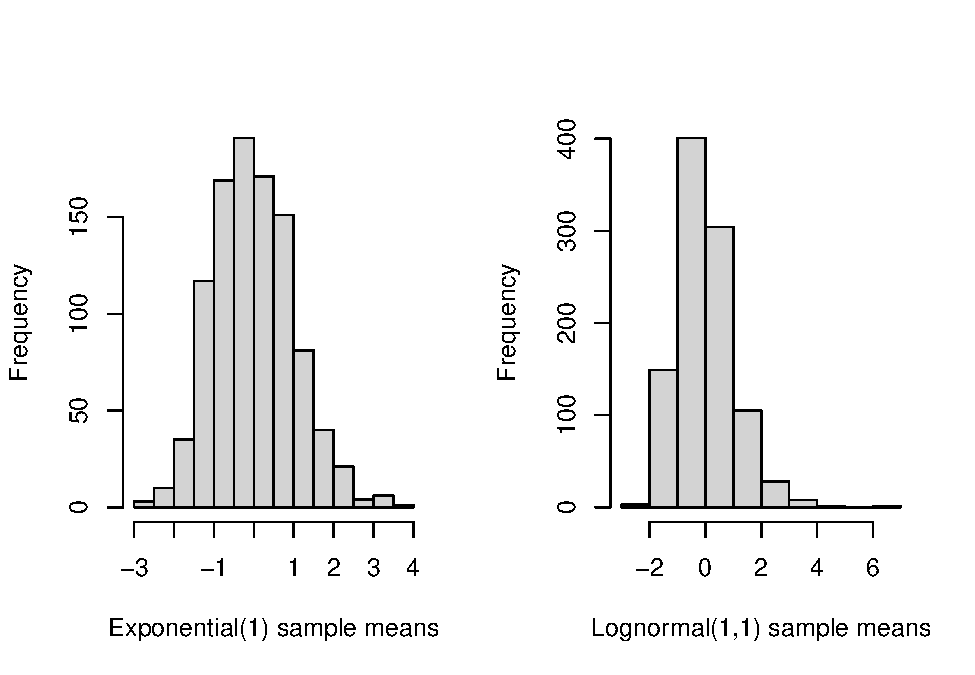
\includegraphics{10-Sampling-Distributions_files/figure-latex/unnamed-chunk-1-2.pdf}

As a final reminder, note the CLT does not apply to ``heavy-tailed'' distributions that lack a mean. For example, the Cauchy distribution is very likely to produce extreme values, and, as a result, it has no finite mean. Therefore, the CLT does not apply and it's unclear what will be the sampling distribution of it's sample mean. It turns out the sample mean is still Cauchy-distributed---taking the average of Cauchy samples does not reduce uncertainty at all. For an illustration, see the Monte-Carlo-approximated distribution of the sample mean of 50 samples from a Cauchy population:

\includegraphics{10-Sampling-Distributions_files/figure-latex/unnamed-chunk-2-1.pdf}

\hypertarget{sample-variance}{%
\section{Sample Variance}\label{sample-variance}}

Let \(X_1, X_2, \ldots, X_n\) denote a random sample from a Normal population with mean \(\mu\) and variance \(\sigma^2\). Denote the sample variance by \(S^2_n = \frac{1}{n-1}\sum_{i=1}^n (X_i - \overline X_n)^2\). Next, we will discover the sampling distribution of the (normal) sample variance.

First, we need to establish the fact that if \(Z\sim N(0,1)\), then \(Z^2\) has what is called a Chi-squared distribution, with one ``degree of freedom''---this is the parameter of this distribution. This Chi-squared distribution has MGF \(\left(1-2t\right)^{-k/2}\) where \(k\) is the degrees of freedom parameter. It's corresponding density function is
\[f(x) = 2^{-k/2}\left[\Gamma(k/2)\right]^{-1}x^{k/2-1}e^{-x/2},\quad x>0\]
and you might recognize this as a Gamma distribution with shape \(k/2\) and rate \(1/2\), so it's mean is \((k/2)/(1/2) = k\). Ww can establish this fact by the MGF technique. Evaluate the MGF of \(Z^2\) as follows:

\begin{align*}
M_{Z^2}(t) &= E(e^{tZ^2}) = \int_{-\infty}^{\infty} e^{tz^2}\frac{1}{\sqrt{2\pi}}e^{-\tfrac12 z^2}dz\\
& = \int_{-\infty}^{\infty} \frac{1}{\sqrt{2\pi}} e^{-\frac{1}{2\frac{1}{1-2t}}z^2}dz\\
& = \sqrt{\frac{1}{1-2t}}\int_{-\infty}^{\infty} \frac{1}{\sqrt{2\pi\frac{1}{1-2t}}} e^{-\frac{1}{2\frac{1}{1-2t}}z^2}dz\\
& = \sqrt{\frac{1}{1-2t}}
\end{align*}
where the last inequality follows from the fact the integrand is a normal density function with mean zero and variance \(\frac{1}{1-2t}\) (provided \(t<2\)) so that the integral equals one. This shows \(Z^2\) is Chi-squared distributed with \(1\) degree of freedom.

As we've many times, the MGF argument works particularly well with sums of independent random variables. If \(Z_1, Z_2, \ldots, Z_n\) are iid standard normal, then \(\sum_{i=1}^n Z_i^2\) is Chi-squared distributed with \(n\) degrees of freedom. To show this, simply show the MGF of \(\sum_{i=1}^n Z_i^2\) equals \(\left(1-2t\right)^{-n/2}\) using the previous result for \(n=1\), the definition of the MGF, and independence.

Next, we'll show a linear transformation of the the sample variance has a Chi-squared distribution with \(n-1\) degrees of freedom.

Start by making the linear transformation
\[\frac{(n-1)S_n^2}{\sigma^2} = \sum_{i=1}^n \left(\frac{X_i - \overline X_n}{\sigma}\right)^2.\]
Here's the main trick: add and subtract \(\mu\) inside the square in the sum, then expand the square and simplify:
\begin{align*}
\frac{(n-1)S_n^2}{\sigma^2} &= \sum_{i=1}^n \left(\frac{X_i - \mu + \mu - \overline X_n}{\sigma}\right)^2\\
& = \sum_{i=1}^n \left(\frac{X_i - \mu}{\sigma}\right)^2 + 2\sum_{i=1}^n \left(\frac{X_i - \mu}{\sigma}\right)\left(\frac{\mu - \overline X_n}{\sigma}\right) + \sum_{i=1}^n \left(\frac{\mu - \overline X_n}{\sigma}\right)^2\\
& = \sum_{i=1}^n \left(\frac{X_i - \mu}{\sigma}\right)^2 - 2n\left(\frac{\overline X_n - \mu}{\sigma}\right)^2 + n\left(\frac{\overline X_n - \mu}{\sigma}\right)^2\\
& = \sum_{i=1}^n \left(\frac{X_i - \mu}{\sigma}\right)^2 - n\left(\frac{\overline X_n - \mu}{\sigma}\right)^2\\
& = \sum_{i=1}^n \left(\frac{X_i - \mu}{\sigma}\right)^2 - \left(\frac{\overline X_n - \mu}{\sigma/\sqrt{n}}\right)^2
\end{align*}

So far, we have shown
\[\sum_{i=1}^n \left(\frac{X_i - \overline X_n}{\sigma}\right)^2 = \sum_{i=1}^n \left(\frac{X_i - \mu}{\sigma}\right)^2 - \left(\frac{\overline X_n - \mu}{\sigma/\sqrt{n}}\right)^2.\]

The first term on the right hand side is a summation of \(n\) squares of independent, standard normal r.v.'s \(Z_i = \frac{X_i - \overline X_n}{\sigma}\). Baed on our previous result, this sum must be distributed as Chi-squared with \(n\) degrees of freedom. The second term on the right is also the square of a standard normal random variable, so it must be distributed as Chi-squared with one degree of freedom. Consequently, the sum on the left hand side must be a Chi-squared random variable with \(n-1\) degrees of freedom.

\hypertarget{large-sample-sampling-distribution-of-sample-variance}{%
\subsection{Large-sample sampling distribution of sample variance}\label{large-sample-sampling-distribution-of-sample-variance}}

If \(X_1, X_2, \ldots, X_n\) is a random sample from a distribution with at least 4 finite moments, then the sample variance \(S_n^2\) is approximately normally distributed for large \(n\). To see this, note
\[S_n^2 = \frac{1}{n-1}\sum_{i=1}^n (X_i - \overline X_n)^2 \approx \frac{1}{n}\sum_{i=1}^n Z_i\]
where \(Z_i = (X_i - \mu)^2\). The latter expression is a sample average of iid random variables, and, as such, the CLT implies (the centered and scaled transformation of) it has a limiting normal distribution. This reasoning can be made rigorous.

\hypertarget{sampling-distribution-of-studentized-sample-mean}{%
\section{Sampling distribution of studentized sample mean}\label{sampling-distribution-of-studentized-sample-mean}}

Let \(X_1, X_2, \ldots, X_n\) be a random sample from a normal population with mean \(\mu\) and variance \(\sigma^2\); and, let \(\overline X_n\) and \(S_n^2\) denote the sample mean and sample variance, respectively.

Let
\[T_n:=\frac{\overline X_n - \mu}{\sqrt{S_n^2 / n}}\]
denote the ``studentized sample mean''. \(T_n\) is the standardized sample mean---\(\overline X_n\) minus \(\mu\) and divided by \(\sqrt{\sigma^2/n}\)---with the true variance replaced by its estimate, the sample variance.

The standardized sample mean has a standard normal distribution (even approximately so for non-normal random samples by the CLT), but the studentized sample mean is \emph{not} normally-distributed. Rather, the studentized sample mean has a Student's \(t\) distribution with \((n-1)\) degrees of freedom.

A Student's \(t\) random variable is defined in the following way: If \(Z\) is standard normal and independent of \(V \sim\) Chi-Squared \((n-1)\), then
\[T:=\frac{Z}{\sqrt{V/(n-1)}}\]
is a Student's \(t\) random variable with \(n-1\) degrees of freedom.

Rewriting the studentized sample mean, we have
\[T_n = \frac{\overline X_n - \mu}{\sqrt{S_n^2 / n}} = \frac{\frac{\overline X_n - \mu}{\sqrt{\sigma^2 / n}}}{\sqrt{(n-1)S_n^2/\{(n-1)\sigma^2\}}} = \frac{Z}{\sqrt{V/(n-1)}}.\]
It remains to verify \(\overline X_n\) and \(S_n^2\) are independent, and a sketch of this result is given next.

\hypertarget{part-of-students-theorem---indepndence-of-overline-x_n-and-s_n2}{%
\subsection{\texorpdfstring{Part of Student's Theorem - Indepndence of \(\overline X_n\) and \(S_n^2\)}{Part of Student's Theorem - Indepndence of \textbackslash overline X\_n and S\_n\^{}2}}\label{part-of-students-theorem---indepndence-of-overline-x_n-and-s_n2}}

Let \(Z_1, \ldots, Z_n\) be a random sample of standard normal random variables. Without loss of generality let's sketch a proof that \(\overline Z_n\) and \(W = \sum_{i=1}^n (Z_i - \overline Z_n)^2\) are independent. Define the matrix \(O_n\) to be the \(n\times n\) matrix with entries defined by:
\[For 1 \leq i \leq n-1, \quad o_{ij} = \Bigg\{ \begin{matrix} \frac{1}{\sqrt{i(i+1)}}, &j\leq i \\
-\frac{1}{\sqrt{i(i+1)}}, &j= i+1 
\end{matrix}\]
and zero otherwise; except that \(o_{nj} = n^{-1/2}\). Then, it can be checked that \(O_n\) is \emph{orthogonal}, i.e., \(O_n^\top O_n = I_n\), the identity. Next, define the vectors \(Z = (Z_1, \ldots, Z_n)^\top\) and \(Y = O_n Z\). By construction of \(O_n\) we have
\[Y^\top Y = Z^\top O_n^\top O_n Z = Z^\top Z = \sum_{i=1}^n Z_i^2.\]
And, we also have
\[Y_n = \sum_{i=1}^n \frac{Z_i}{\sqrt{n}} = \sqrt{n} \overline Z_n.\]
Therefore,
\[\sum_{i=1}^{n-1}Y_i^2 = \sum_{i=1}^{n}Y_i^2 - Y_n^2 = Z^\top Z - n\overline Z_n^2 = W.\]
So far, we have shown \(\overline Z_n\) is a function of \(Y_n\) and \(W\) is a function of \(Y_1, \ldots, Y_{n-1}\). But, \(Y = O_n Z\) is normally distributed with covariance \(O_n^\top O_n = I_n\). Therefore, \(Y_i\), \(i=1, \ldots, n\), are independent, which implies \(\overline Z_n\) and \(W\) are independent.

\hypertarget{differences-of-sample-means}{%
\section{Differences of Sample Means}\label{differences-of-sample-means}}

So far we have considered statistics baed on a single random sample. Now, we'll consider statistics based on separate random samples from two populations. First, consider a random sample \(X_1, X_2, \ldots, X_{n}\) from a normal distribution with mean and variance \(\mu_X\) and \(\sigma_X^2\) and another random sample \(Y_1, Y_2, \ldots, Y_m\) from a different normal distribution with mean and variance \(\mu_Y\) and \(\sigma_Y^2\).

\hypertarget{standarized-difference}{%
\subsection{Standarized difference}\label{standarized-difference}}

The standardized difference of means is given by
\[Z = \frac{\overline X_n - \overline Y_m - (\mu_X - \mu_Y)}{\sqrt{\frac{\sigma_X^2}{n} + \frac{\sigma_Y^2}{m}}}\]
and follows a standard normal distribution.

\hypertarget{studentized-difference-equal-variances}{%
\subsection{Studentized difference, equal variances}\label{studentized-difference-equal-variances}}

Suppose \(\sigma_X^2 = \sigma_Y^2\), and define the \emph{pooled sample variance} \(S_P^2 = \frac{(n-1)S_X^2 + (m-1)S_Y^2}{n+m-2}\). The studentized difference of sample means is defined by
\[T = \frac{\overline X_n - \overline Y_m - (\mu_X - \mu_Y)}{\sqrt{S_p^2(\frac{1}{n}+\frac{1}{m})}}\]
follows a Student's \(t\) distribution with \(n+m - 2\) degrees of freedom.

\hypertarget{studentized-difference-unequal-variances}{%
\subsection{Studentized difference, unequal variances}\label{studentized-difference-unequal-variances}}

When the population variances are unequal a different version of the studentized difference of means is sometimes used:
\[T = \frac{\overline X_n - \overline Y_m - (\mu_X - \mu_Y)}{\sqrt{\frac{S_X^2}{n}+\frac{S_Y^2}{m}}}.\]
This difference does not have an exact \(t\) distribution, but can be approximated well by a \(t\) distribution with degrees of freedom given by Satterthwaite's formula:
\[df = \frac{\left(\frac{S_X^2}{n}+\frac{S_Y^2}{m}\right)^2}{\frac{1}{n-1}\left(\frac{S_X^2}{n}\right)^2 + \frac{1}{m-1}\left(\frac{S_Y^2}{m}\right)^2}.\]
Since the degrees of freedom is an integer-valued parameter the result of this formula is \emph{rounded down} to the nearest integer.

\hypertarget{ratios-of-sample-variances}{%
\section{Ratios of Sample Variances}\label{ratios-of-sample-variances}}

As above, consider a random sample \(X_1, X_2, \ldots, X_{n}\) from a normal distribution with mean and variance \(\mu_X\) and \(\sigma_X^2\) and another random sample \(Y_1, Y_2, \ldots, Y_m\) from a different normal distribution with mean and variance \(\mu_Y\) and \(\sigma_Y^2\).

If \(U\sim\) Chi-Squared with df \(n-1\) and \(V\sim\) Chi-Squared with df \(m-1\) and \(U\) and \(V\) are independent, then
\[F := \frac{U/(n-1)}{V/(m-1)}\]
has an F distribution with two degrees of freedom parameters \(df1 = n-1\) and \(df2 = m-1\), often called the numerator and denominator degrees of freedom.

If \(S_X^2\) and \(S_Y^2\) are sample variances, then
\[\frac{\frac{(n-1)S_X^2}{\sigma_X^2(n-1)}}{\frac{(m-1)S_Y^2}{\sigma_Y^2(m-1)}} = \frac{S_X^2/\sigma_X^2}{S_Y^2/\sigma_Y^2}\]
has an \(F(n-1, m-1)\) distribution.

\hypertarget{confidence-intervals}{%
\chapter{Confidence Intervals}\label{confidence-intervals}}

\hypertarget{why-want-interval-valued-estimates}{%
\section{Why want interval-valued estimates?}\label{why-want-interval-valued-estimates}}

Point estimators, like the sample mean, certainly help to describe features of the population. But, the trouble with point estimators is that, on their own, they provide no sense of uncertainty. On one hand, a point estimator is just one number, and one number seems very precise. So, in a sort of psychological sense (and I'm being very loose with that term) people may feel a false sense of certainty about a point estimate. For example, if I say ``the sample mean is 5'' someone could very reasonably expect the population mean is quite close to 5, but, given a little intuition, that person's opinion may change quite a bit depending on whether the sample size is, say, 10 or 100. On the other hand, in a mathematical statistical sense, we know an estimator is a random variable with a distribution that, usually, has a finite variance. And, if known, we could use knowledge of that distribution to quantify the variability (read uncertainty) inherent in the estimator. So, besides the point estimate itself, it would be helpful to report some measure of variability of the estimate to give the user a more informed view of the estimate of the population mean (or other feature being estimated).

One way to include information of the uncertainty of a point estimate is to include an estimate of the estimator's standard deviation---this is usually called a ``standard error''. For example, the sample mean \(\overline X_n\) estimates the population mean \(\mu\) and if the population has a finite variance \(\sigma^2\) then the standard deviation of \(\overline X_n\) is \(\sigma/\sqrt{n}\). Usually, \(\sigma^2\) is unknown, so it is replaced by a point estimate, say, the usual sample variance \(S_n^2 = \frac{1}{n-1}\sum_{i=1}^n (X_i - \overline X_n)^2\) to get the standard error \(\sqrt{S_n^2/n}\). A common practice is to report the estimate \(\overline x_n\) along with the standard error \(s_n/\sqrt{n}\).

One drawback of reporting an estimate and its standard deviation is that it's not clear how much variability one standard deviation really represents; it depends on the sampling distribution of the estimator. For example, if an estimator is normally distributed then an interval of one standard deviation about its mean contains about \(68\%\) of the distribution, and see the figure below. One the other hand, suppose an estimator has a Chi-squared distribution with \(5\) degrees of freedom. Then an interval of radius one standard deviation about its mean contains about \(72\%\) of the distribution. The point is that one standard deviation does not provide an objective summary of uncertainty across different distributions.

\includegraphics{12-Confidence-Intervals_files/figure-latex/unnamed-chunk-1-1.pdf}

To remedy this issue of the vagueness of standard deviation/standard error we introduce the concept of a confidence interval. An interval-valued estimate is an interval or range of values representing a set that may plausibly contain the true parameter value. Let's denote this interval by \((\ell, u)\), its lower and upper bounds. Then, a reasonable way to define the endpoints is to select them so that the interval has the \emph{confidence property}
\[P(\ell \leq \theta \leq u) = 1-\alpha\]
where \(\theta\) is the true parameter value and \(\alpha \in (0,1)\) is up to the user to decide---usually \(\alpha\) is near zero. The probability statement is with respect to \(\ell\) and \(u\), meaning these endpoints are random variables---in particular, they should be statistics, i.e., depended on the data. Then, a \emph{confidence interval} is a random interval with a prescribed chance of ``catching'' the true parameter.

\hypertarget{normal-population-mean-example}{%
\section{Normal population mean example}\label{normal-population-mean-example}}

Suppose \(X_1, \ldots, X_n\) is a random sample from \(N(\mu, 1)\). Let's find a \(100(1-\alpha)\%\) confidence interval (CI) for \(\mu\). Since \(\overline X_n\) is a great estimator of \(\mu\) it makes sense the endpoints of the interval would depend on \(\overline X_n\). The confidence interval is supposed to be a range of plausible values of \(\mu\); and, \(\overline X_n\) seems the most plausible, so the interval ought to look like \((\overline X_n - c_1, \, \overline X_n + c_2)\); in other words, the interval is the sample mean plus or minus something extra. We known \(\overline X_n \sim N(\mu, 1/n)\), which is a symmetric distribution. So, it would make sense for our \(\pm \text{ something extra}\) to be symmetric, i.e.~the interval should have the form \((\overline X_n - c, \overline X_n + c)\) for some \(c>0\). Now, it just remains to specify \(c\) such that the interval has the confidence property. We want
\[P(\overline X_n - c \leq \mu \leq \overline X_n +c) = 1-\alpha.\]
Subtract \(\overline X_n\) and standardize to get the standard normal probability
\[P\left(-\frac{c}{1/\sqrt{n}} \leq \frac{\overline X_n - \mu}{1/\sqrt{n}} \leq \frac{c}{1/\sqrt{n}}\right) = 1-\alpha\]
\[P\left(-\frac{c}{1/\sqrt{n}} \leq Z \leq \frac{c}{1/\sqrt{n}}\right) = 1-\alpha.\]
This means \(P(Z\leq \frac{c}{1/\sqrt{n}}) = 1-\alpha/2\) by symmetry of the standard normal distribution. In other words, \(\frac{c}{1/\sqrt{n}}\) is the value such that
\[1-\alpha/2=F_Z(\frac{c}{1/\sqrt{n}})=\int_{-\infty}^{\frac{c}{1/\sqrt{n}}} \frac{1}{\sqrt{2\pi}}e^{-\frac{1}{2}z^2}dz.\]
This defines \(\frac{c}{1/\sqrt{n}}\) as the \(1-\alpha/2\) standard normal quantile. Given a choice of \(\alpha\) it's not easy to solve for \(c\) in the above (integral) equation, but we can use the built-in R function qnorm to find this value. Let \(\alpha = 0.025\), for example, so that the probability our interval contains \(\mu\) is \(95\%\). Then, \(\frac{c}{1/\sqrt{n}} = qnorm(0.975) = 1.96\) and \(c = 1.96\frac{1}{\sqrt{n}}\). Conclude a \(95\%\) CI for \(\mu\) is given by
\[\left(\overline X_n - 1.96\frac{1}{\sqrt{n}}, \,\overline X_n - 1.96\frac{1}{\sqrt{n}}\right).\]
More generally, if we denote the \(1-\alpha/2\) quantile of the standard normal by \(z_{1-\alpha/2}\) then
\[\left(\overline X_n - z_{1-\alpha/2}\frac{1}{\sqrt{n}}, \,\overline X_n - z_{1-\alpha/2}\frac{1}{\sqrt{n}}\right)\]
defines a \(100(1-\alpha)\%\) CI for \(\mu\).

Remark: It's not essential that the above CI (or any CI) is symmetric about a point estimator, but when the sampling distribution of the estimator is symmetric this is the best choice. To see this, note that
\[\left(\overline X_n - z_{1-\alpha/3}\frac{1}{\sqrt{n}}, \,\overline X_n - z_{1-2\alpha/3}\frac{1}{\sqrt{n}}\right)\]
is also a \(95\%\) CI for \(\mu\), but it is \emph{always} larger (wider) than the symmetric interval. So, the symmetric interval, which being shorter is more precise, is preferable.

\hypertarget{other-exact-cis-for-normal-population-mean-and-variance-parameters}{%
\section{Other ``Exact'' CIs for normal population mean and variance parameters}\label{other-exact-cis-for-normal-population-mean-and-variance-parameters}}

\hypertarget{population-mean-unknown-variance}{%
\subsection{Population mean, unknown variance}\label{population-mean-unknown-variance}}

Let \(X_1, \ldots, X_n\) be a random sample of size \(n\geq 2\) from \(N(\mu, \sigma^2)\) where both mean and variance parameters are unknown. We know the studentized mean follows a Student's \(t\) distribution with \(n-1\) degrees of freedom:
\[T = \frac{\overline X_n - \mu}{\sqrt{S_n^2/n}}\sim t(n-1).\]
Mirroring the argument from above when \(\sigma^2\) is a known value, we assume a \(100(1-\alpha)\%\) CI for \(\mu\) would be symmetric about \(\overline X_n\) with radius \(t_{1-\alpha/2}(n-1) \frac{S_n}{\sqrt{n}}\) where \(t_{1-\alpha/2}(n-1)\) is the \(1-\alpha/2\) quantile of the Student's \(t\) distribution with \(n-1\) degrees of freedom:
\[P\left(\overline X_n - t_{1-\alpha/2}(n-1) \frac{S_n}{\sqrt{n}} \leq \mu \leq \overline X_n + t_{1-\alpha/2}(n-1) \frac{S_n}{\sqrt{n}}\right) = 1-\alpha.\]

\hypertarget{population-variance-unknown-mean}{%
\subsection{Population variance, unknown mean}\label{population-variance-unknown-mean}}

Let \(X_1, \ldots, X_n\) be a random sample of size \(n\geq 2\) from \(N(\mu, \sigma^2)\) where both mean and variance parameters are unknown. We know the following transformation is Chi-squared distributed:
\[\frac{(n-1)S_n^2)}{\sigma^2}\sim \chi^2(n-1).\]
Now, the Chi-squared distribution is not symmetric---it's skewed. There are a number of ways to define a \(100(1-\alpha)\%\) CI for \(\sigma^2\) based on the above sampling distribution. Since \(\sigma^2 > 0\) we can define a one-sided interval starting from zero:
\[\left(0, \, \frac{(n-1)S_n^2}{\chi^2_{\alpha}(n-1)}\right)\]
where \(\chi^2_{1-\alpha}(n-1)\) is the \(100(1-\alpha)\) quantile of a Chi-squared r.v. with \((n-1)\) degrees of freedom. Then,
\begin{align*}
P(0 \leq \sigma^2 \leq \frac{(n-1)S_n^2}{\chi^2_{\alpha}(n-1)}) &= P(0\leq \frac{(n-1)S_n^2}{\sigma^2} \leq \chi^2_{1-\alpha}(n-1))\\
& = P(\chi^2(n-1) \geq \chi^2_{\alpha}(n-1))\\
&= 1-\alpha
\end{align*}
by definition of the quantile.

We can define two-sided intervals as well. The ``equi-tailed'' interval is not the shortest possible interval, but it has a simple form:
\[\left(\frac{(n-1)S_n^2}{\chi^2_{1-\alpha/2}(n-1)}, \, \frac{(n-1)S_n^2}{\chi^2_{\alpha/2}(n-1)}\right).\]

In order to find the shortest possible \(100(1-\alpha)\%\) CI one could draw a horizontal line slicing across the Chi-squared density such that the area under both the line and the density equals \(\alpha\). Then, the intersection points of the line and the density would give the lower and upper Chi-squared quantiles to use in the two-sided interval. Since the density is not symmetric this interval generally would not be based on the \(1-\alpha/2\) and \(\alpha/2\) quantiles like the equi-tailed interval. For example, the shortest \(95\%\) CI when \(df=10\) is based on quantile values of about 1.284 and 25.05. The following plot illustrates this.

\begin{verbatim}
## 0.04998856 with absolute error < 8.5e-05
\end{verbatim}

\begin{verbatim}
## [1] 0.001862438
\end{verbatim}

\begin{verbatim}
## [1] 0.001863508
\end{verbatim}

\includegraphics{12-Confidence-Intervals_files/figure-latex/unnamed-chunk-2-1.pdf}

\hypertarget{two-normal-samples-comparing-means}{%
\subsection{Two normal samples, comparing means}\label{two-normal-samples-comparing-means}}

Let's tackle the next topic by way of an example. Suppose infant walking time --- the age in months at which babies can walk on their own --- is normally distributed. Generally, parents are excited for their infants to begin walking and some parents ``take steps'' to encourage their infants to walk. We'll assume it is reasonable to model the population of infant walking times among those infants whose parents no not intervene in walking skills development as a random sample from a normal distribution with mean \(\mu_x\) and variance \(sigma_x^2\); likewise we model the corresponding population of infant walking times influenced by parent behavior by a normal distribution with mean \(\mu_y\) and variance \(sigma_y^2\). Assume this parental influence factor represents a more-or-less standard ``treatment''; for example, parents might spend 60 minutes a day encouraging their infant to crawl and stand with assistance or play in a bounce seat to build lower body strength. Child development researchers would be interested to know whether such parental interventions influence infant walking times.

Given observations from an experiment comparing these two groups of infants, how would we answer the researchers' question? One answer comes in the form of a CI for the difference of means \(\mu_x - \mu_y\). In this case a negative difference indicates some impact of parental involvement. And, if a \(95\%\) CI does not contain zero, then the CI reflects strong evidence in the data that the true means are different.

Based on our knowledge of sampling distributions we know that if \(\sigma_x^2 = \sigma_y^2\) the following statistic has a Student's \(t\) distribution with \(n+m-2\) df where \(n\) and \(m\) are the sample sizes in each group:
\[\frac{\overline X - \overline Y - (\mu_x - \mu_y)}{\sqrt{S_p^2\left(\frac{1}{n} + \frac{1}{m}\right)}}\]
where \(S_p^2\) denotes the pooled (sample-size weighted average) sample variance. As a result, the following probability statement is exact:
\begin{align*}
1-\alpha & = P\left(t_{\alpha/2, n+m-2} \leq \frac{\overline X - \overline Y - (\mu_x - \mu_y)}{\sqrt{S_p^2\left(\frac{1}{n} + \frac{1}{m}\right)}} \leq t_{1-\alpha/2, n+m-2}\right)\\
& = P\left(t_{\alpha/2, n+m-2}\sqrt{S_p^2\left(\frac{1}{n} + \frac{1}{m}\right)}\leq \overline X - \overline Y - (\mu_x - \mu_y) \leq t_{1-\alpha/2, n+m-2}\sqrt{S_p^2\left(\frac{1}{n} + \frac{1}{m}\right)}\right)\\
& = P\left(-(\overline X - \overline Y)+t_{\alpha/2, n+m-2}\sqrt{S_p^2\left(\frac{1}{n} + \frac{1}{m}\right)}\leq  - (\mu_x - \mu_y) \leq -(\overline X - \overline Y)+ t_{1-\alpha/2, n+m-2}\sqrt{S_p^2\left(\frac{1}{n} + \frac{1}{m}\right)}\right)\\
& = P\left((\overline X - \overline Y)-t_{1-\alpha/2, n+m-2}\sqrt{S_p^2\left(\frac{1}{n} + \frac{1}{m}\right)}\leq   (\mu_x - \mu_y) \leq (\overline X - \overline Y)+ t_{1-\alpha/2, n+m-2}\sqrt{S_p^2\left(\frac{1}{n} + \frac{1}{m}\right)}\right)
\end{align*}
where the last line follows from multiplying by \(-1\) and noting \(t_{1-\alpha/2, n+m-2} = -t_{\alpha/2, n+m-2}\) by symmetry. Therefore, a \(100(1-\alpha)\%\) CI for the difference of means \(\mu_x - \mu_y\) is given by
\[\left((\overline X - \overline Y)-t_{1-\alpha/2, n+m-2}\sqrt{S_p^2\left(\frac{1}{n} + \frac{1}{m}\right)}, \, (\overline X - \overline Y)+t_{1-\alpha/2, n+m-2}\sqrt{S_p^2\left(\frac{1}{n} + \frac{1}{m}\right)}\right).\]
Suppose we conduct the infant walking time experiment and observe the following data:
\[X:\,\,\, 13.2\,\,\, 16.6\,\,\, 16.7\,\,\, 16.8\,\,\, 17.0\,\,\, 17.1\,\,\, 17.3\,\,\, 17.4\,\,\, 17.4\,\,\, 17.7\,\,\, 17.9 \]
\[Y: \,\,\, 16.8\,\,\, 17.1\,\,\, 17.6\,\,\, 17.7\,\,\, 18.8\,\,\, 18.8\,\,\, 19.3\,\,\, 19.6\,\,\, 21.0\,\,\, 21.2\,\,\, 21.5\,\,\, 22.1\,\,\, 22.8\]
Computing the sample statistics we find \(\overline x = 16.83\), \(\overline y = 19.56\), \(s_x^2 = 1.61\), and \(s_y^2 = 3.97\). The pooled sample variance is \((10s_x^2+12s_y^2)/22 = 2.90\). The \(0.975\) quantile of the Student's \(t\) distribution with 22 df can be found using ``qt(0.975, 22)'' and equals about 2.07. Plugging all these values into the CI formula, the \(95\%\) CI for the difference in mean infant walking times is\\
\[(-4.18, \, -1.29)\]
We conclude the mean infant walking times in the group with parental intervention were between about 1.3 and 4.2 months shorter than in the non-intervention group. (Note this is made-up ``data'' only for illustration purposes.)

The careful reader may be concerned that our CI method used above relies on the two normal populations having identical variances but our sample variances are substantially different. This equal-variance CI procedure is often referred to as Students's two-sample CI, in contrast to an alternative method that can be used when variances are unequal called Welch's two-sample CI. Recall the studentized difference of sample means when variances are unequal approximately (not exactly) follows a Student's \(t\) distribution with Satterthwaite's choice of degrees of freedom:
\[\frac{\overline X_n - \overline Y_m - (\mu_X - \mu_Y)}{\sqrt{\frac{S_X^2}{n}+\frac{S_Y^2}{m}}}\stackrel{\cdot}{\sim}t(\nu)\]
where
\[\nu = \frac{\left(\frac{S_X^2}{n}+\frac{S_Y^2}{m}\right)^2}{\frac{1}{n-1}\left(\frac{S_X^2}{n}\right)^2 + \frac{1}{m-1}\left(\frac{S_Y^2}{m}\right)^2}.\]
Following the same argument as above, this implies an \emph{approximate} \(100(1-\alpha)\%\) CI for the difference of means is given by
\[\left((\overline X - \overline Y)-t_{1-\alpha/2, \nu}\sqrt{\left(\frac{S_x^2}{n} + \frac{S_y^2}{m}\right)}, \, (\overline X - \overline Y)+t_{1-\alpha/2, \nu}\sqrt{S_p^2\left(\frac{S_x^2}{n} + \frac{S_y^2}{m}\right)}\right).\]
Plugging in the relevant sample statistics, we get \(\nu = 20\) so that we use the quantile \(t_{0.975}(20) = 2.086\). Welch's two-sample approximate \(95\%\) interval is
\[(-4.14, \,-1.33)\]
which is hardly different than Student's interval. We'll investigate the comparative performances of these two intervals further in lab.

\hypertarget{two-normal-samples-comparing-variances}{%
\subsection{Two normal samples, comparing variances}\label{two-normal-samples-comparing-variances}}

In some applications it is either more important or at least of equal importance to compare population variances rather than means. For example, consider one or more manufacturing processes for producing optical lenses---these might be for glasses or contacts. Lenses have many dimensional quantities that determine their properties, for example, the refraction index of the lens material and the thickness of the lens, which both contribute to the power of the lens. Suppose a manufacturing process is supposed to produce a lens of a given thickness. A small tolerance is allowable but any lenses produced with thickness outside the tolerance must be rejected. We can think of the difference between the specified, target lens thickness and the population mean thickness of lenses produced by a specific process as \emph{bias}. Then, our preference between two or more production processes is a question about bias-variance tradeoff. A production process with no bias but a high variance in lens thickness will result in many lenses being rejected---perhaps even more than a manufacturing process that produces biased lenses with very low variability in thickness. Clearly, for choosing between processes we need to evaluate both process bias and process variance.

For comparing two process variances (where the underlying popualtions are normal) we use a ratio statistic. The sampling distribution of the following ratio of sample variances has an \emph{F distribution} when the population variances are equal:
\[\frac{S_x^2}{S_y^2} \sim F(n-1, m-1).\]
Recall that \((n-1)S_x^2/\sigma_x^2 \sim\) Chi-squared\((n-1)\) and \((m-1)S_y^2/\sigma_y^2 \sim\) Chi-squared\((m-1)\). The ratio of two independent, Chi-squared r.v.'s divided by the dfs defines an F random variable with two parameters which are the degrees of freedom of the numerator and denominator Chi-squared r.v.'s. When \(\sigma_x^2 = \sigma_y^2\), we have
\[\frac{\frac{(n-1)S_x^2}{\sigma_x^2(n-1)}}{\frac{(m-1)S_y^2}{\sigma_y^2(m-1)}} = \frac{\frac{(n-1)S_x^2}{(n-1)}}{\frac{(m-1)S_y^2}{(m-1)}} = \frac{\text{Chi-squared(n-1)/(n-1)}}{\text{Chi-squared(m-1)/(m-1)}} = \frac{S_x^2}{S_y^2} =  F(n-1, m-1).\]
And, when the variances are not equal, we simply have
\[\frac{S_x^2 \sigma_y^2}{S_y^2 \sigma_x^2} \sim F(n-1, m-1).\]
We can invert this relationship to find a CI for \(\sigma_y^2 / \sigma_x^2\) using the following probability computation:
\begin{align*}
1-\alpha & = P(F_{\alpha/2}(n-1, m-1) \leq \frac{S_x^2 \sigma_y^2}{S_y^2 \sigma_x^2} \leq F_{1-\alpha/2}(n-1, m-1))\\
& = P(\frac{S_y^2}{S_x^2}F_{\alpha/2}(n-1, m-1) \leq \sigma_y^2/\sigma_x^2 \leq \frac{S_y^2}{S_x^2}F_{1-\alpha/2}(n-1, m-1))\\
& = P(\frac{S_y^2}{S_x^2}\frac{1}{F_{1-\alpha/2}(m-1, n-1)} \leq \sigma_y^2/\sigma_x^2 \leq \frac{S_y^2}{S_x^2}F_{1-\alpha/2}(n-1, m-1)),
\end{align*}
where the last line uses a reciprocal-equality property of F distributions with swapped degrees of freedom, namely \(F_{\alpha}(df1, df2) = 1/(F_{1-\alpha}(df2, df1))\). This is not essential if you are using R to compute F quantiles but is helpful for using F tables, which typically only list upper tail quantiles. Then, a \(100(1-\alpha)\%\) CI for the ratio \(\sigma_y^2/\sigma_x^2\) is given by
\[\left(\frac{S_y^2}{S_x^2}\frac{1}{F_{1-\alpha/2}(m-1, n-1)}, \,\frac{S_y^2}{S_x^2}F_{1-\alpha/2}(n-1, m-1)\right).\]
Given the following observations (in nanometers) of lens thickness using two different production methods, compute \(95\%\) CIs for the difference in means (use Welch's method) and the ratio of variances:
\[X: 2.9859\,\,\, 3.0042\,\,\, 3.0055 \,\,\,3.0083 \,\,\,3.0113 \,\,\,3.0124\,\,\, 3.0150\,\,\, 3.0214\]
\[Y: 2.9964\,\,\, 3.0011 \,\,\,3.0099\,\,\, 3.0110\,\,\, 3.0124\,\,\, 3.0130\,\,\, 3.0140\,\,\, 3.0205\]
The \(95\%\) CI for the difference in population mean thicknesses is
\[(-0.0116, \, 0.0080).\]
The \(95\%\) CI for the ratio of population variances \(\sigma_y^2/\sigma_x^2\) is
\[(0.1058, \, 2.6394).\]

\hypertarget{cis-for-proportions}{%
\section{CIs for proportions}\label{cis-for-proportions}}

\hypertarget{a-single-bernoulli-proportion}{%
\subsection{A single Bernoulli proportion}\label{a-single-bernoulli-proportion}}

Using the DeMoivre-Laplace CLT we know the standardized sample proportion is approximately normally distributed:

\[\frac{\hat p - p}{\sqrt{\frac{p(1-p)}{n}}}\stackrel{\cdot}{\sim}N(0,1)\]

Then, again denoting lower standard normal quantiles by \(z_\alpha\), we have
\[1-\alpha \approx P\left(z_{\alpha/2} \leq \frac{\hat p - p}{\sqrt{\frac{p(1-p)}{n}}}\leq z_{1-\alpha/2}\right).\]

As in other cases covered above, we can derive an approximate CI for \(p\) by algebraic manipulations within the probability statement. A complicating factor is that the true proportion \(p\) shows up in both the numerator and denominator of the standardized sample proportion. A common technique to get around this is to replace the standard deviation of \(\hat p\) by the estimated standard deviation \(\sqrt{\hat p(1-\hat p)/n}\). Using the estimated standard deviation, an approximate \(100(1-\alpha)\%\) CI for \(p\) is given by
\[\left(\hat p + z_{\alpha/2}\sqrt{\frac{\hat p(1-\hat p)}{n}}, \, \hat p + z_{1-\alpha/2}\sqrt{\frac{\hat p(1-\hat p)}{n}}\right).\]

It is possible to derive a CI for \(p\) without resorting to using the estimated standard deviation. In that case, we have to solve for \(p\) in the quadratic equation
\[\frac{\hat p - p}{\sqrt{\frac{p(1-p)}{n}}}= z_{1-\alpha/2}.\]
The endpoints of the CI based on the true standard deviation of \(\hat p\) are given by
\[\frac{n\hat p + 0.5z_{\alpha/2}^2\pm z_{1-\alpha/2}\sqrt{n\hat p(1-\hat p)+0.25z_{\alpha/2}^2}}{n+z_{\alpha/2}^2}.\]

Example: A survey is conducted to determine the level of support for the construction of a new nuclear power plant in a community. 140 of 400 randomly sampled voters favor the construction project. Find a \(99\%\) approximate CI for the true proportion of voters favoring the project.
The sample proportion is \(\hat p = 0.35\) and the estimated standard deviation of \(\hat p\) is \(\sqrt{0.35\cdot 0.65 / 400} = 0.02384848\). Given \(z_{0.995} = 2.575\) an approximate \(99\%\) CI for p is given by
\[(28.86\%, \, 41.14\%).\]

Alternatively, using the formula for the CI based on the true standard deviation of \(\hat p\) we find the interval
\[(29.15\%, \, 41.34\%).\]

\hypertarget{difference-of-two-bernoulli-proportions}{%
\subsection{Difference of two Bernoulli proportions}\label{difference-of-two-bernoulli-proportions}}

The most common experiments compare two or more populations. For two Bernoulli populations an approximate CI for the difference of population proportions can be computed based on the DeMoivre-Laplace CLT similarly to the single population interval above based on the estimated standard deviation of the sample proportion. Our CI for the difference of proportions is given by
\[\left(\hat p_1 - \hat p_2 + z_{\alpha/2}\sqrt{\frac{\hat p_1(1-\hat p_1)}{n_1} + \frac{\hat p_2(1-\hat p_2)}{n_2}}, \,\,\,\,\, \hat p_1 - \hat p_2 + z_{1-\alpha/2}\sqrt{\frac{\hat p_1(1-\hat p_1)}{n_1} + \frac{\hat p_2(1-\hat p_2)}{n_2}}\right).\]
Example: Suppose a poll of Illinois voters finds 132 of 200 male voters and 90 of 150 female voters favor a certain candidate. A \(99\%\) CI for the difference of population favorability proportions between the sexes is
\[(-7.4\%, \, 19.4\%)\]
indicating there is, plausibly, no difference in the candidate's favorability between the sexes.

\hypertarget{approximate-cis-based-on-mles}{%
\section{Approximate CIs based on MLEs}\label{approximate-cis-based-on-mles}}

So far we have derived CIs for parameters based on sampling distributions of statistics used to estimate those parameters. We can use the same strategy to derive CIs for parameters estimated using maximum likelihood whenever asymptotic normality of the corresponding MLE is justified. Recall there are a few cases where asymptotic normality may not hold, such as estimating the lower or upper bounds of a uniform distribution---that case violates the condition that the sample space does not depend on the parameter. However, in many situations asymptotic normality of the MLE does hold, and we can use it to derive approximate CIs.

Recall that, under some regularity conditions, the MLE \(\hat\theta\) for the scalar parameter \(\theta\) is approximately normally distributed with mean \(\theta\) and variance \([nI(\theta)]^{-1}\) where \(I(\theta)\) is the Fisher information for one sample. If we replace the variance by the estimated variance by plugging in \(\hat\theta\) then we obtain the CI
\[\left(\hat\theta \pm z_{1-\alpha/2}[nI(\hat\theta)]^{-1/2}\right),\]
where you'll recall that \(I(\theta) = E\left[\left(\frac{\partial \ell}{\partial \theta}\right)^2\right]\) or, equivalently (most of the time), \(I(\theta) = -E\left(\frac{\partial^2 \ell}{\partial \theta^2}\right)\) where \(\ell\) denotes the loglikelihood function.

Example: The MLE of the exponential rate parameter is \(\hat\theta = \overline X\). We have previously found \([nI(\theta)]^{-1/2} = \sqrt{(\overline X)^2/n}\) so that an MLE-based approximate CI for the exponential rate \(\theta\) is given by
\[\left(\overline X \pm z_{1-\alpha/2}\frac{\overline X}{\sqrt{n}}\right).\]

\hypertarget{multivariate-case}{%
\subsection{Multivariate case}\label{multivariate-case}}

When \(\theta\) is a vector parameter the MLE \(\hat\theta\) is approximately distributed as a multivariate normal random vector with mean vector \(\theta\) and (estimated) covariance matrix \([nI(\hat\theta)]^{-1}\). We can compute approximate CIs for each element of \(\theta\) using the marginal approximate normal distributions of the elements of \(\hat\theta\) as in the scalar case. However, we can also compute a joint confidence region for two or more elements of \(\theta\). The elliptical region
\[\{\theta: (\hat \theta - \theta)[nI(\hat\theta)]^{-1}(\hat \theta - \theta)^\top \leq z_{1-\alpha/2}^2\}\]
is an approximate \(100(1-\alpha)\%\) confidence region for \(\theta\). It is also smaller than the set product of marginal confidence intervals, which is a hyper-rectangle containing this ellipse.

Example: The MLEs for a normal population mean and variance have approximate normal distribution
\[(\overline X, \hat\sigma^2) \stackrel{\cdot}{\sim}N\left((\mu, \sigma^2), \begin{bmatrix} \sigma^2/n & 0 \\ 0 & 2\sigma^4/n \end{bmatrix}\right).\]
An approximate \(100(1-\alpha)\%\) elliptical confidence region for \((\mu, \sigma^2)\) is given by
\[\{(\mu, \sigma^2): (\overline X - \mu, \hat\sigma^2 - \sigma^2)\begin{bmatrix} \hat\sigma^2/n & 0 \\ 0 & 2\hat\sigma^4/n \end{bmatrix}^{-1} (\overline X - \mu, \hat\sigma^2 - \sigma^2)^\top \leq z_{1-\alpha/2}^2\}.\]

\begin{Shaded}
\begin{Highlighting}[]
\FunctionTok{set.seed}\NormalTok{(}\DecValTok{56482}\NormalTok{)}
\NormalTok{data }\OtherTok{\textless{}{-}} \FunctionTok{rnorm}\NormalTok{(}\DecValTok{20}\NormalTok{, }\DecValTok{5}\NormalTok{, }\DecValTok{3}\NormalTok{)}
\NormalTok{xbar }\OtherTok{\textless{}{-}} \FunctionTok{mean}\NormalTok{(data)}
\NormalTok{s2 }\OtherTok{\textless{}{-}} \FunctionTok{var}\NormalTok{(data)}\SpecialCharTok{*}\NormalTok{(}\DecValTok{19}\NormalTok{)}\SpecialCharTok{/}\DecValTok{20}

\NormalTok{xc }\OtherTok{\textless{}{-}}\NormalTok{ xbar }\CommentTok{\# center x\_c or h}
\NormalTok{yc }\OtherTok{\textless{}{-}}\NormalTok{ s2 }\CommentTok{\# y\_c or k}
\NormalTok{a }\OtherTok{\textless{}{-}} \FloatTok{1.96}\SpecialCharTok{*}\FunctionTok{sqrt}\NormalTok{(s2}\SpecialCharTok{/}\DecValTok{20}\NormalTok{) }\CommentTok{\# major axis length}
\NormalTok{b }\OtherTok{\textless{}{-}}  \FloatTok{1.96}\SpecialCharTok{*}\FunctionTok{sqrt}\NormalTok{(}\DecValTok{2}\SpecialCharTok{*}\NormalTok{(s2}\SpecialCharTok{\^{}}\DecValTok{2}\NormalTok{)}\SpecialCharTok{/}\DecValTok{20}\NormalTok{) }\CommentTok{\# minor axis length}
\NormalTok{phi }\OtherTok{\textless{}{-}} \DecValTok{0} \CommentTok{\# angle of major axis with x axis phi or tau}

\NormalTok{t }\OtherTok{\textless{}{-}} \FunctionTok{seq}\NormalTok{(}\DecValTok{0}\NormalTok{, }\DecValTok{2}\SpecialCharTok{*}\NormalTok{pi, }\FloatTok{0.01}\NormalTok{) }
\NormalTok{x }\OtherTok{\textless{}{-}}\NormalTok{ xc }\SpecialCharTok{+}\NormalTok{ a}\SpecialCharTok{*}\FunctionTok{cos}\NormalTok{(t)}\SpecialCharTok{*}\FunctionTok{cos}\NormalTok{(phi) }\SpecialCharTok{{-}}\NormalTok{ b}\SpecialCharTok{*}\FunctionTok{sin}\NormalTok{(t)}\SpecialCharTok{*}\FunctionTok{sin}\NormalTok{(phi)}
\NormalTok{y }\OtherTok{\textless{}{-}}\NormalTok{ yc }\SpecialCharTok{+}\NormalTok{ a}\SpecialCharTok{*}\FunctionTok{cos}\NormalTok{(t)}\SpecialCharTok{*}\FunctionTok{sin}\NormalTok{(phi) }\SpecialCharTok{+}\NormalTok{ b}\SpecialCharTok{*}\FunctionTok{sin}\NormalTok{(t)}\SpecialCharTok{*}\FunctionTok{cos}\NormalTok{(phi)}
\FunctionTok{plot}\NormalTok{(x,y, }\AttributeTok{col=}\StringTok{\textquotesingle{}blue\textquotesingle{}}\NormalTok{,  }\AttributeTok{type =} \StringTok{\textquotesingle{}l\textquotesingle{}}\NormalTok{, }\AttributeTok{xlim =} \FunctionTok{c}\NormalTok{(}\DecValTok{3}\NormalTok{,}\DecValTok{7}\NormalTok{), }\AttributeTok{ylim =} \FunctionTok{c}\NormalTok{(}\DecValTok{2}\NormalTok{,}\DecValTok{15}\NormalTok{))}

\NormalTok{CI.mu }\OtherTok{\textless{}{-}} \FunctionTok{c}\NormalTok{(xbar }\SpecialCharTok{{-}} \FloatTok{1.96}\SpecialCharTok{*}\FunctionTok{sqrt}\NormalTok{(s2}\SpecialCharTok{/}\DecValTok{20}\NormalTok{), xbar }\SpecialCharTok{+} \FloatTok{1.96}\SpecialCharTok{*}\FunctionTok{sqrt}\NormalTok{(s2}\SpecialCharTok{/}\DecValTok{20}\NormalTok{))}
\NormalTok{CI.sig2 }\OtherTok{\textless{}{-}} \FunctionTok{c}\NormalTok{(s2 }\SpecialCharTok{{-}} \FloatTok{1.96}\SpecialCharTok{*}\FunctionTok{sqrt}\NormalTok{(}\DecValTok{2}\SpecialCharTok{*}\NormalTok{(s2}\SpecialCharTok{\^{}}\DecValTok{2}\NormalTok{)}\SpecialCharTok{/}\DecValTok{20}\NormalTok{), s2 }\SpecialCharTok{+} \FloatTok{1.96}\SpecialCharTok{*}\FunctionTok{sqrt}\NormalTok{(}\DecValTok{2}\SpecialCharTok{*}\NormalTok{(s2}\SpecialCharTok{\^{}}\DecValTok{2}\NormalTok{)}\SpecialCharTok{/}\DecValTok{20}\NormalTok{))}

\FunctionTok{lines}\NormalTok{(}\FunctionTok{c}\NormalTok{(CI.mu[}\DecValTok{1}\NormalTok{], CI.mu[}\DecValTok{2}\NormalTok{]),}\FunctionTok{c}\NormalTok{(CI.sig2[}\DecValTok{1}\NormalTok{], CI.sig2[}\DecValTok{1}\NormalTok{]), }\AttributeTok{col =} \StringTok{\textquotesingle{}red\textquotesingle{}}\NormalTok{) }
\FunctionTok{lines}\NormalTok{(}\FunctionTok{c}\NormalTok{(CI.mu[}\DecValTok{1}\NormalTok{], CI.mu[}\DecValTok{2}\NormalTok{]),}\FunctionTok{c}\NormalTok{(CI.sig2[}\DecValTok{2}\NormalTok{], CI.sig2[}\DecValTok{2}\NormalTok{]), }\AttributeTok{col =} \StringTok{\textquotesingle{}red\textquotesingle{}}\NormalTok{) }
\FunctionTok{lines}\NormalTok{(}\FunctionTok{c}\NormalTok{(CI.mu[}\DecValTok{1}\NormalTok{], CI.mu[}\DecValTok{1}\NormalTok{]),}\FunctionTok{c}\NormalTok{(CI.sig2[}\DecValTok{1}\NormalTok{], CI.sig2[}\DecValTok{2}\NormalTok{]), }\AttributeTok{col =} \StringTok{\textquotesingle{}red\textquotesingle{}}\NormalTok{) }
\FunctionTok{lines}\NormalTok{(}\FunctionTok{c}\NormalTok{(CI.mu[}\DecValTok{2}\NormalTok{], CI.mu[}\DecValTok{2}\NormalTok{]),}\FunctionTok{c}\NormalTok{(CI.sig2[}\DecValTok{1}\NormalTok{], CI.sig2[}\DecValTok{2}\NormalTok{]), }\AttributeTok{col =} \StringTok{\textquotesingle{}red\textquotesingle{}}\NormalTok{) }
\end{Highlighting}
\end{Shaded}

\includegraphics{12-Confidence-Intervals_files/figure-latex/unnamed-chunk-3-1.pdf}

\hypertarget{the-delta-method}{%
\subsection{The Delta method}\label{the-delta-method}}

The delta theorem says that asymptotic normality of the MLE is preserved under smooth (differentiable) transformations. Let \(g(\cdot)\) be a differentiable function. Then,
\[\sqrt{n}(g(\hat\theta) - g(\theta))\stackrel{\cdot}{\sim} N\left(0, [g'(\theta)]^\top I(\theta)^{-1}g'(\theta)\right).\]

The power of the delta theorem is its implied method for constructing CIs for any ``nice'' function of population parameters.

Example: For a normal population experiment a common function of parameters that is of interest to researchers is the so-called ``signal-to-noise ratio'' given by \(\mu/\sigma\). In this case, \(g(\theta) = g(\mu, \sigma^2) = \mu/\sqrt{\sigma^2}\). And, \(g'(\theta) = (1/\sqrt{\sigma^2},\, -0.5\mu/({(\sigma^2)}^{1.5}))\). Using the delta theorem result, the MLE of \(\mu/\sigma\) is given by \(\overline X / \sqrt{\hat\sigma^2}\) and has approximate variance
\[(1/\sqrt{\hat\sigma^2},\, -0.5\overline X/({(\hat\sigma^2)}^{1.5})) \begin{bmatrix} \hat\sigma^2/n & 0 \\ 0 & 2\hat\sigma^4/n \end{bmatrix} (1/\sqrt{\hat\sigma^2},\, -0.5\overline X/({(\hat\sigma^2)}^{1.5}))^\top = \frac{1}{n}+\frac{\overline X^2}{2n\hat\sigma^2}.\]
Then, an approximate CI for \(\mu/\sigma\) is given by
\[\left(\overline X / \sqrt{\hat\sigma^2} \pm z_{1-\alpha/2}\sqrt{\frac{1}{n}+\frac{\overline X^2}{2n\hat\sigma^2}}\right).\]

\hypertarget{hypothesis-testing}{%
\chapter{Hypothesis Testing}\label{hypothesis-testing}}

So far our discussion of statistical inference has been limited to ``estimation'', which is essentially any method that determines which parameter values match/agree with observed data. We have discussed both parametric and non-parametric estimation, although we have not used those terms. Non-parametric estimation refers to estimation of population parameters without specifying any probability model for the data. For example, the sample mean is a reasonable estimator of the population mean (should it exist) regardless of the sampling distribution of the data (the population distribution). Parametric estimators are tied to assumed sampling distributions. For example, maximum likelihood estimators totally rely on an assumed sampling distribution of the data (population distribution). Parametric estimation can be viewed as selecting which particular probability model within a given set (the assumed distribution) best fits the data.

We'll next expand our discussion of statistical inference to ask a different, but related question. Instead of asking which parameters/model distributions agree with a given data set, we ask ``how much evidence does a given data set provide for a particular parameter value or set of parameter values?'' The particular parameter values are referred to as the hypothesis or ``null hypothesis''. And, a procedure that determines whether the data provides sufficient evidence against the null hypothesis so as to make it implausible is called a ``hypothesis test''.

\hypertarget{notation}{%
\section{Notation}\label{notation}}

Consider a generic parameter \(\theta\) taking values in some set \(\Theta\). The null hypothesis \(\theta\) takes exactly the value \(\theta_0\) is written \(H_0: \theta = \theta_0\). Its complement is the alternative hypothesis \(H_a: \theta\ne\theta_0\), which is always the set complement of the null hypothesis. In particular, \(H_0: \theta = \theta_0\) is called a ``point-null hypothesis'' because the set in the null hypothesis consists of only a single point. In other cases, the null hypothesis is ``composite'', e.g., \(H_0:\theta \leq \theta_0\) versus \(H_a: \theta > \theta_0\).

Example: Suppose an experiment consist of collecting a random sample from a normal population with unknown mean \(\mu\) and unknown variance \(\sigma^2\). A point null hypothesis that \(\mu = 0\) is phrased \(H_0: \mu = 0\) versus the alternative hypothesis \(\mu \ne 0\). A point null hypothesis that \(\sigma^2 = 1\) is phrased \(H_0:\sigma^2=1\) versus \(H_a:\sigma^2 \ne 1\), where the alternative hypothesis tacitly assumes \(\sigma^2>0\).

\hypertarget{hypothesis-testing-outcomes}{%
\section{Hypothesis testing outcomes}\label{hypothesis-testing-outcomes}}

A hypothesis testing procedure begins with a pair of null and alternative hypotheses. Next, data relevant to the hypotheses is collected, and a decision is made as to whether the data provides sufficient evidence against the null hypothesis such that it may be rejected as implausible. Otherwise, the data are viewed as sufficiently consistent with the null hypothesis as to retain it.

As such, there are four possible outcomes of this procedure. In two cases, the correct decision is made: either the null hypothesis is true and it is retained, or the null hypothesis is false and it is reject. There are two corresponding errors:
1) A Type 1 error is committed when the null hypothesis is true but it is rejected; and,
2) A Type 2 error is committed when the null hypothesis is false and it is retained.

Since the decision to reject or retain the null hypothesis is based on a random sample of data, the decision is itself random; so, each of these outcomes has a certain probability of occuring. Given the null hypothesis is true, the chance of a Type 1 error occurring is denoted \(\alpha\) and is also called the Type 1 error rate. Given the null hypothesis is false the chance of a Type 2 error occurring is denoted \(\beta\), and its complement, the chance of rejecting \(H_0\) is denoted \(1-\beta\) and referred to as the ``power of the test''.

Of course, it would be nice if one could eliminate any chance of an error occurring, but that is not possible. To see this, consider the extreme case of a non-random hypothesis test that always rejects the null hypothesis, no matter the data. Such a rule minimizes the chance of a Type 2 error (in fact there is such chance) but maximizes the chance of a Type 1 error. And, the opposite extreme, in which the null hypothesis is always retained similarly minimizes Type 1 error at the cost of maximizing Type 2 errors. Any testing procedure in between necessarily has some positive chance of each type of error.

As we will see, it is possible to construct hypothesis tests with an explicit cap (upper bound) on the Type 1 error rate \(\alpha\). This means that, whenever possible, it makes sense to design experiments and hypotheses such that Type 1 errors are more serious than Type 2 errors, so that they may be expressly controlled. A hypothesis test that limits \(\alpha\) to a prespecified level is called a ``level-\(\alpha\) test''.

\hypertarget{tests-based-on-a-normal-population}{%
\section{Tests based on a normal population}\label{tests-based-on-a-normal-population}}

\hypertarget{test-for-a-normal-mean-when-the-variance-is-known}{%
\subsection{Test for a normal mean when the variance is known}\label{test-for-a-normal-mean-when-the-variance-is-known}}

Suppose a given population is known to follow a normal distribution with an unknown mean and a known variance \(\sigma^2\). We wish to test the point null hypothesis \(H_0:\mu = \mu_0\) for some given number \(\mu_0\) versus the alternative \(H_a:\mu \ne \mu_0\). And, we wish our test to limit the Type 1 error rate to a given level \(\alpha\), say, \(5\%\).

We obtain a random sample of size \(n\) from the population. How should we proceed? If \(H_0\) is true, then our data should look like it came from \(N(\mu_0, \sigma^2)\); specifically, the sample mean should be ``close'' to \(\mu_0\). If \(\overline X\) is close to \(\mu_0\), then \(H_0\) seems plausible, otherwise not. Our intuition says our test should look like: ``reject \(H_0\) if \(|\overline X-\mu_0|>c\)'' for some cutoff \(c>0\). The constraint on Type 1 error rate to be no more than \(\alpha\) is enough to determine \(c\):
\begin{align*}
1-\alpha &= P(-c\leq \overline X - \mu_0 \leq c)\\
& = P(-c/\sqrt{\sigma^2/n} \leq Z \leq c/\sqrt{\sigma^2/n})
\end{align*}
This implies we should reject \(H_0\) if \(|Z|>z_{1-\alpha/2}\) where
\[Z = \frac{\overline X - \mu_0}{\sqrt{\sigma^2/n}}\]
is the standardized sample mean assuming \(H_0\) is true (often it is said, ``under \(H_0\)'').

Next, we investigate the power of this test. Recall the power is the probability the test rejects the null hypothesis when the null is false. For most tests, like the current one, the null hypothesis may be false in many ways. If \(H_0\) is false then \(\mu\ne \mu_0\), so \(\mu\) is some other number, lets say \(y\). Intuitively, for \(y\) values close to \(\mu_0\) we would not necessarily expect to notice \(H_0\) is false, but for \(y\) values far from \(\mu_0\) we would expect \(\overline X\) to be far from \(\mu_0\) and for the test to reject \(\mu_0\). So, we expect the power to be a function of \(y\) and to be increasing as a function of \(|y-\mu_0|\). Below we compute this power function:
\begin{align*}
P\left(\frac{\overline X - \mu_0}{\sigma/\sqrt{n}} < z_{\alpha/2}|\mu = y\right) & =  P\left(\frac{\overline X - y}{\sigma/\sqrt{n}} < z_{\alpha/2}+\frac{\mu_0-y}{\sigma/\sqrt{n}}\right)\\
& = P\left(Z < z_{\alpha/2}+\frac{\mu_0-y}{\sigma/\sqrt{n}}\right).
\end{align*}
\begin{align*}
P\left(z_{1-\alpha/2} < \frac{\overline X - \mu_0}{\sigma/\sqrt{n}}|\mu = y\right) & =  P\left(z_{1-\alpha/2}+\frac{\mu_0-y}{\sigma/\sqrt{n}}<\frac{\overline X - y}{\sigma/\sqrt{n}}\right)\\
& = P\left(z_{1-\alpha/2}+\frac{\mu_0-y}{\sigma/\sqrt{n}} < Z\right)\\
& = 1-P\left(Z < z_{1-\alpha/2}+\frac{\mu_0-y}{\sigma/\sqrt{n}}\right).
\end{align*}
Therefore, the power as a function of \(y\) is
\[(1-\beta) = P\left(Z < z_{\alpha/2}+\frac{\mu_0-y}{\sigma/\sqrt{n}}\right)+1-P\left(Z < z_{1-\alpha/2}+\frac{\mu_0-y}{\sigma/\sqrt{n}}\right).\]
We illustrate this power function below for \(H_0:\mu = 1\) where \(\sigma^2 = 2\), \(n=10\), and \(\alpha = 0.05\).

\begin{Shaded}
\begin{Highlighting}[]
\NormalTok{alpha }\OtherTok{\textless{}{-}} \FloatTok{0.05}
\NormalTok{mu0 }\OtherTok{\textless{}{-}} \DecValTok{1}
\NormalTok{sigma2 }\OtherTok{\textless{}{-}} \DecValTok{2}
\NormalTok{n }\OtherTok{\textless{}{-}} \DecValTok{10}
\NormalTok{power }\OtherTok{\textless{}{-}} \ControlFlowTok{function}\NormalTok{(y) }\FunctionTok{pnorm}\NormalTok{(}\FunctionTok{qnorm}\NormalTok{(alpha}\SpecialCharTok{/}\DecValTok{2}\NormalTok{)}\SpecialCharTok{+}\NormalTok{(}\DecValTok{1}\SpecialCharTok{{-}}\NormalTok{y)}\SpecialCharTok{/}\FunctionTok{sqrt}\NormalTok{(sigma2}\SpecialCharTok{/}\NormalTok{n))}\SpecialCharTok{+}\DecValTok{1}\SpecialCharTok{{-}}\FunctionTok{pnorm}\NormalTok{(}\FunctionTok{qnorm}\NormalTok{(}\DecValTok{1}\SpecialCharTok{{-}}\NormalTok{alpha}\SpecialCharTok{/}\DecValTok{2}\NormalTok{)}\SpecialCharTok{+}\NormalTok{(}\DecValTok{1}\SpecialCharTok{{-}}\NormalTok{y)}\SpecialCharTok{/}\FunctionTok{sqrt}\NormalTok{(sigma2}\SpecialCharTok{/}\NormalTok{n))}
\FunctionTok{curve}\NormalTok{(power, }\AttributeTok{from =} \SpecialCharTok{{-}}\DecValTok{5}\NormalTok{, }\AttributeTok{to =} \DecValTok{6}\NormalTok{, }\AttributeTok{xlab =} \StringTok{\textquotesingle{}y\textquotesingle{}}\NormalTok{, }\AttributeTok{ylab =} \StringTok{\textquotesingle{}power(y)\textquotesingle{}}\NormalTok{)  }
\end{Highlighting}
\end{Shaded}

\includegraphics{13-Hypothesis-Testing_files/figure-latex/unnamed-chunk-1-1.pdf}

The power is minimized (and equal to 0.05) at \(y = \mu_0\) where the test only rejects at rate \(\alpha\) by design. The power increases smoothly and symetrically as a function of \(|y-\mu_0|\) until the test has nearly a \(100\%\) chance of rejecting \(H_0\) for true mean sufficiently far from \(\mu_0\).

\hypertarget{test-for-a-normal-mean-when-the-variance-is-unknown}{%
\subsection{Test for a normal mean when the variance is unknown}\label{test-for-a-normal-mean-when-the-variance-is-unknown}}

As we have discussed many times when the population variance is unknown the Studentized sample mean has a Student's \(t\) distribution with \(n-1\) degrees of freedom. A Student's \(t-\)based test for \(H_0:\mu = \mu_0\) versus \(H_a:\mu\ne\mu_0\) is essentially the same as the above test but based on the \(T\) statistic, \(T = \frac{\overline X - \mu_0}{S/\sqrt{n}}\) rather than the \(Z\) statistic \(Z = \frac{\overline X - \mu_0}{\sigma/\sqrt{n}}\). A level-\(\alpha\) test rejects \(H_0\) if \(T > t_{1-\alpha/2}(n-1)\) or \(T < t_{\alpha/2}(n-1)\), where \(t_\alpha(df)\) is the Student's \(t\) lower \(\alpha\) quantile with \(df\) degrees of freedom.

For a different angle, consider the test of the one-sided (composite) hypotheses \(H_0:\mu \leq \mu_0\) versus \(H_a:\mu > \mu_0\). Naturally, values of \(\overline X\) smaller than \(\mu_0\) lend support to the null hypothesis, so a level \(\alpha\) test of \(H_0\) only rejects the null if \(T > t_{1-\alpha}(n-1)\). Consider the power of this one-sided test. Since the test only rejects for large values of \(\overline X\), the power should increase as \(T\) increases. Mimicking (half of) our power calculation for the \(Z\) test above we have
\[1-\beta = P\left(\frac{\overline X - y}{S/\sqrt{n}} + \frac{y - \mu_0}{S/\sqrt{n}} > t_{1-\alpha}(n-1)\right).\]
The random variable \(\frac{\overline X - y}{S/\sqrt{n}} + \frac{y - \mu_0}{S/\sqrt{n}}\) has a Student's \(t\) distribution with \(n-1\) degrees of freedom and \textbf{non-centrality parameter} \((y-\mu_0)/(\sigma / \sqrt{n})\).

\begin{Shaded}
\begin{Highlighting}[]
\NormalTok{alpha }\OtherTok{\textless{}{-}} \FloatTok{0.05}
\NormalTok{mu0 }\OtherTok{\textless{}{-}} \DecValTok{1}
\NormalTok{sigma2 }\OtherTok{\textless{}{-}} \DecValTok{2}
\NormalTok{n }\OtherTok{\textless{}{-}} \DecValTok{10}
\NormalTok{power }\OtherTok{\textless{}{-}} \ControlFlowTok{function}\NormalTok{(y)  }\DecValTok{1}\SpecialCharTok{{-}}\FunctionTok{pt}\NormalTok{(}\FunctionTok{qt}\NormalTok{(}\DecValTok{1}\SpecialCharTok{{-}}\NormalTok{alpha, n}\DecValTok{{-}1}\NormalTok{), }\AttributeTok{df =}\NormalTok{ n}\DecValTok{{-}1}\NormalTok{, }\AttributeTok{ncp =}\NormalTok{ (y }\SpecialCharTok{{-}}\NormalTok{ mu0)}\SpecialCharTok{/}\NormalTok{(}\FunctionTok{sqrt}\NormalTok{(sigma2}\SpecialCharTok{/}\NormalTok{n)))}
\FunctionTok{curve}\NormalTok{(power, }\AttributeTok{from =} \SpecialCharTok{{-}}\DecValTok{1}\NormalTok{, }\AttributeTok{to =} \DecValTok{4}\NormalTok{, }\AttributeTok{xlab =} \StringTok{\textquotesingle{}y\textquotesingle{}}\NormalTok{, }\AttributeTok{ylab =} \StringTok{\textquotesingle{}power(y)\textquotesingle{}}\NormalTok{)  }
\end{Highlighting}
\end{Shaded}

\includegraphics{13-Hypothesis-Testing_files/figure-latex/unnamed-chunk-2-1.pdf}

\begin{Shaded}
\begin{Highlighting}[]
\FunctionTok{power}\NormalTok{(}\DecValTok{2}\NormalTok{)}
\end{Highlighting}
\end{Shaded}

\begin{verbatim}
## [1] 0.6623762
\end{verbatim}

Here's a quick simulation to illustrate the above power function: we'll sample data sets of \(n=10\) samples from \(N(\mu = 2, \sigma^2 = 2)\) a total of 10000 times. Each time we'll compute the p-value of the test \(H_0:\mu \leq 1\) versus \(H_a:\mu > 1\). According to the above power calculation, we should reject \(H_0\) about two thirds of the time if \(\alpha = 0.05\).

\begin{Shaded}
\begin{Highlighting}[]
\NormalTok{res }\OtherTok{\textless{}{-}} \FunctionTok{rep}\NormalTok{(}\ConstantTok{NA}\NormalTok{,}\DecValTok{10000}\NormalTok{)}
\ControlFlowTok{for}\NormalTok{(i }\ControlFlowTok{in} \DecValTok{1}\SpecialCharTok{:}\DecValTok{10000}\NormalTok{)\{}
\NormalTok{  x }\OtherTok{\textless{}{-}} \FunctionTok{rnorm}\NormalTok{(n,}\DecValTok{2}\NormalTok{,}\FunctionTok{sqrt}\NormalTok{(sigma2))}
\NormalTok{  res[i] }\OtherTok{=} \FunctionTok{t.test}\NormalTok{(x,}\AttributeTok{mu =}\NormalTok{ mu0,}\AttributeTok{alternative =} \StringTok{"greater"}\NormalTok{)}\SpecialCharTok{$}\NormalTok{p.value}
\NormalTok{\}}
\FunctionTok{sum}\NormalTok{(res}\SpecialCharTok{\textless{}}\FloatTok{0.05}\NormalTok{)}\SpecialCharTok{/}\DecValTok{10000}
\end{Highlighting}
\end{Shaded}

\begin{verbatim}
## [1] 0.6604
\end{verbatim}

\hypertarget{test-for-a-normal-population-variance}{%
\subsection{Test for a normal population variance}\label{test-for-a-normal-population-variance}}

Consider a test that rejects the null hypothesis \(H_0:\sigma^2 \leq \sigma_0^2\) if \(\frac{(n-1)S^2}{\sigma_0^2} \geq \chi^2_{1-\alpha}(n-1)\) where \(\chi^2_{\alpha}(df)\) is the Chi-squared lower \(\alpha\) quantile for a Chi-squared distribution with df degrees of freedom. Such a rejection rule defines a level-\(\alpha\) test:
\[P\left(\frac{(n-1)S^2}{\sigma_0^2} \geq  \chi^2_{1-\alpha}(n-1)|\sigma^2 = \sigma_0^2\right) = P\left(\chi^{2}(n-1) \geq  \chi^2_{1-\alpha}(n-1)\right) = \alpha,\]
by definition. We can compute the power curve of such a test:
\begin{align*}
P\left(\frac{(n-1)S^2}{\sigma_0^2} \geq  \chi^2_{1-\alpha}(n-1)|\sigma^2 = y\right) & = P\left(\frac{(n-1)S^2}{y} \geq  \frac{\sigma_0^2}{y}\chi^2_{1-\alpha}(n-1)\right)\\
& = P\left(\chi^2(n-1) \geq  \frac{\sigma_0^2}{y}\chi^2_{1-\alpha}(n-1)\right)
\end{align*}

\begin{Shaded}
\begin{Highlighting}[]
\NormalTok{alpha }\OtherTok{\textless{}{-}} \FloatTok{0.05}
\NormalTok{mu0 }\OtherTok{\textless{}{-}} \DecValTok{1}
\NormalTok{sigma2 }\OtherTok{\textless{}{-}} \DecValTok{2}
\NormalTok{n }\OtherTok{\textless{}{-}} \DecValTok{10}
\NormalTok{power }\OtherTok{\textless{}{-}} \ControlFlowTok{function}\NormalTok{(y)  }\DecValTok{1}\SpecialCharTok{{-}}\FunctionTok{pchisq}\NormalTok{((}\DecValTok{2}\SpecialCharTok{/}\NormalTok{y)}\SpecialCharTok{*}\FunctionTok{qchisq}\NormalTok{(}\DecValTok{1}\SpecialCharTok{{-}}\NormalTok{alpha, n}\DecValTok{{-}1}\NormalTok{),n}\DecValTok{{-}1}\NormalTok{)}
\FunctionTok{curve}\NormalTok{(power, }\AttributeTok{from =} \DecValTok{2}\NormalTok{, }\AttributeTok{to =} \DecValTok{14}\NormalTok{, }\AttributeTok{xlab =} \StringTok{\textquotesingle{}y\textquotesingle{}}\NormalTok{, }\AttributeTok{ylab =} \StringTok{\textquotesingle{}power(y)\textquotesingle{}}\NormalTok{)  }
\end{Highlighting}
\end{Shaded}

\includegraphics{13-Hypothesis-Testing_files/figure-latex/unnamed-chunk-4-1.pdf}

\hypertarget{example-the-lifetimes-of-infected-guinea-pigs}{%
\subsection{Example: The lifetimes of infected Guinea pigs}\label{example-the-lifetimes-of-infected-guinea-pigs}}

58 Guinea pigs were infected with a bacilli (bacteria) to determine its effect on lifespan. The control group of non-infected Guinea pigs lived on average 325 days. We'll test whether the infected pigs live, on average, less than 325 days. A comparative boxplot does not show any indications of non-normality in the lifetimes, so a t-test is reasonable. Based on the extreme test statistic (-5.33) and the tiny p-value (\textless0.0001) we conclude the infected pigs live, on average, less than 325 days. As this was a randomized experiment, it is reasonable to conclude the treatment/infection with bacilli is the cause of the reduced average lifespan. And, provided there is no reason to suspect these Guinea pigs are somehow different than Guinea pigs in general, we could assume the same results would hold, generally, in the (hypothetical) population of all Guinea pigs.

\begin{Shaded}
\begin{Highlighting}[]
\NormalTok{pigs }\OtherTok{\textless{}{-}} 
\FunctionTok{read.csv}\NormalTok{(}\StringTok{\textquotesingle{}E:}\SpecialCharTok{\textbackslash{}\textbackslash{}}\StringTok{Teaching}\SpecialCharTok{\textbackslash{}\textbackslash{}}\StringTok{STAT500}\SpecialCharTok{\textbackslash{}\textbackslash{}}\StringTok{MyMaterials}\SpecialCharTok{\textbackslash{}\textbackslash{}}\StringTok{Homework}\SpecialCharTok{\textbackslash{}\textbackslash{}}\StringTok{guinea\_pigs.csv\textquotesingle{}}\NormalTok{)}
\FunctionTok{boxplot}\NormalTok{(Time}\SpecialCharTok{\textasciitilde{}}\NormalTok{Treatment, }\AttributeTok{data=}\NormalTok{pigs)}
\end{Highlighting}
\end{Shaded}

\includegraphics{13-Hypothesis-Testing_files/figure-latex/unnamed-chunk-5-1.pdf}

\begin{Shaded}
\begin{Highlighting}[]
\NormalTok{mu0 }\OtherTok{\textless{}{-}} \DecValTok{325}
\NormalTok{m\_C }\OtherTok{\textless{}{-}} \FunctionTok{mean}\NormalTok{(pigs}\SpecialCharTok{$}\NormalTok{Time[pigs}\SpecialCharTok{$}\NormalTok{Treatment }\SpecialCharTok{==} \StringTok{"Control"}\NormalTok{])}
\NormalTok{m\_C}
\end{Highlighting}
\end{Shaded}

\begin{verbatim}
## [1] 345.2188
\end{verbatim}

\begin{Shaded}
\begin{Highlighting}[]
\NormalTok{m\_B }\OtherTok{\textless{}{-}} \FunctionTok{mean}\NormalTok{(pigs}\SpecialCharTok{$}\NormalTok{Time[pigs}\SpecialCharTok{$}\NormalTok{Treatment }\SpecialCharTok{==} \StringTok{"Bacilli"}\NormalTok{])}
\NormalTok{m\_B}
\end{Highlighting}
\end{Shaded}

\begin{verbatim}
## [1] 242.5345
\end{verbatim}

\begin{Shaded}
\begin{Highlighting}[]
\NormalTok{s\_B }\OtherTok{\textless{}{-}} \FunctionTok{sd}\NormalTok{(pigs}\SpecialCharTok{$}\NormalTok{Time[pigs}\SpecialCharTok{$}\NormalTok{Treatment }\SpecialCharTok{==} \StringTok{"Bacilli"}\NormalTok{])}
\NormalTok{s\_B}
\end{Highlighting}
\end{Shaded}

\begin{verbatim}
## [1] 117.9309
\end{verbatim}

\begin{Shaded}
\begin{Highlighting}[]
\NormalTok{n\_B }\OtherTok{\textless{}{-}} \FunctionTok{sum}\NormalTok{(pigs}\SpecialCharTok{$}\NormalTok{Treatment }\SpecialCharTok{==} \StringTok{"Bacilli"}\NormalTok{)}
\NormalTok{n\_B}
\end{Highlighting}
\end{Shaded}

\begin{verbatim}
## [1] 58
\end{verbatim}

\begin{Shaded}
\begin{Highlighting}[]
\FunctionTok{c}\NormalTok{(m\_B }\SpecialCharTok{+} \FunctionTok{qt}\NormalTok{(}\FloatTok{0.05}\NormalTok{, n\_B }\SpecialCharTok{{-}} \DecValTok{1}\NormalTok{)}\SpecialCharTok{*}\NormalTok{s\_B}\SpecialCharTok{/}\FunctionTok{sqrt}\NormalTok{(n\_B), m\_B }\SpecialCharTok{+} \FunctionTok{qt}\NormalTok{(}\FloatTok{0.95}\NormalTok{, n\_B }\SpecialCharTok{{-}} 
\DecValTok{1}\NormalTok{)}\SpecialCharTok{*}\NormalTok{s\_B}\SpecialCharTok{/}\FunctionTok{sqrt}\NormalTok{(n\_B))}
\end{Highlighting}
\end{Shaded}

\begin{verbatim}
## [1] 216.643 268.426
\end{verbatim}

\begin{Shaded}
\begin{Highlighting}[]
\NormalTok{t.stat }\OtherTok{\textless{}{-}}\NormalTok{ (m\_B }\SpecialCharTok{{-}}\NormalTok{ mu0)}\SpecialCharTok{/}\NormalTok{(s\_B}\SpecialCharTok{/}\FunctionTok{sqrt}\NormalTok{(n\_B))}
\NormalTok{t.stat}
\end{Highlighting}
\end{Shaded}

\begin{verbatim}
## [1] -5.325481
\end{verbatim}

\begin{Shaded}
\begin{Highlighting}[]
\FunctionTok{pt}\NormalTok{(t.stat, n\_B}\DecValTok{{-}1}\NormalTok{)}
\end{Highlighting}
\end{Shaded}

\begin{verbatim}
## [1] 8.875078e-07
\end{verbatim}

\begin{Shaded}
\begin{Highlighting}[]
\NormalTok{dt1 }\OtherTok{\textless{}{-}} \ControlFlowTok{function}\NormalTok{(x) }\FunctionTok{dt}\NormalTok{(x, n\_B }\SpecialCharTok{{-}} \DecValTok{1}\NormalTok{)}
\FunctionTok{curve}\NormalTok{(dt1, }\SpecialCharTok{{-}}\DecValTok{6}\NormalTok{,}\DecValTok{6}\NormalTok{, }\AttributeTok{xlab =} \StringTok{"Test Statistic"}\NormalTok{, }\AttributeTok{ylab =} \StringTok{"Density"}\NormalTok{, }\AttributeTok{main =} \StringTok{"Null Distribution Student\textquotesingle{}s t(57)"}\NormalTok{)}
\FunctionTok{abline}\NormalTok{(}\AttributeTok{v =}\NormalTok{ t.stat, }\AttributeTok{col =} \StringTok{\textquotesingle{}red\textquotesingle{}}\NormalTok{)}
\FunctionTok{abline}\NormalTok{(}\AttributeTok{v =} \FunctionTok{qt}\NormalTok{(}\FloatTok{0.05}\NormalTok{, n\_B}\DecValTok{{-}1}\NormalTok{), }\AttributeTok{col =} \StringTok{\textquotesingle{}blue\textquotesingle{}}\NormalTok{)}
\end{Highlighting}
\end{Shaded}

\includegraphics{13-Hypothesis-Testing_files/figure-latex/unnamed-chunk-5-2.pdf}

Next, we note the standard deviation of lifetime in the control group is about 222 days. One might expect the infected group to have a lover standard deviation of lifetime given many will die prematurely. Let's test \(H_0: \sigma \geq 222\) versus \(H_0: \sigma < 222\) using a the pivotal quantity \(\frac{(n-1)S^2}{\sigma_0^2} \sim \chi^2(n-1)\)---this null hypothesis test statistic has a Chi-squared distribution with \(n-1\) degrees of freedom. Based on the very small p-value, we reject the null hypothesis. For reference, the figure below shows the test statistic (red) and \(\alpha =0.05\) cutoff (blue) in relation to the null distribution of the test statistic.

\begin{Shaded}
\begin{Highlighting}[]
\NormalTok{s\_B }\OtherTok{\textless{}{-}} \FunctionTok{sd}\NormalTok{(pigs}\SpecialCharTok{$}\NormalTok{Time[pigs}\SpecialCharTok{$}\NormalTok{Treatment }\SpecialCharTok{==} \StringTok{"Bacilli"}\NormalTok{])}
\NormalTok{s\_B}
\end{Highlighting}
\end{Shaded}

\begin{verbatim}
## [1] 117.9309
\end{verbatim}

\begin{Shaded}
\begin{Highlighting}[]
\NormalTok{n\_B }\OtherTok{\textless{}{-}} \FunctionTok{sum}\NormalTok{(pigs}\SpecialCharTok{$}\NormalTok{Treatment }\SpecialCharTok{==} \StringTok{"Bacilli"}\NormalTok{)}
\NormalTok{n\_B}
\end{Highlighting}
\end{Shaded}

\begin{verbatim}
## [1] 58
\end{verbatim}

\begin{Shaded}
\begin{Highlighting}[]
\FunctionTok{c}\NormalTok{((n\_B }\SpecialCharTok{{-}} \DecValTok{1}\NormalTok{)}\SpecialCharTok{*}\NormalTok{(s\_B}\SpecialCharTok{\^{}}\DecValTok{2}\NormalTok{)}\SpecialCharTok{/}\FunctionTok{qchisq}\NormalTok{(}\FloatTok{0.975}\NormalTok{, n\_B }\SpecialCharTok{{-}} \DecValTok{1}\NormalTok{), (n\_B }\SpecialCharTok{{-}} \DecValTok{1}\NormalTok{)}\SpecialCharTok{*}\NormalTok{(s\_B}\SpecialCharTok{\^{}}\DecValTok{2}\NormalTok{)}\SpecialCharTok{/}\FunctionTok{qchisq}\NormalTok{(}\FloatTok{0.025}\NormalTok{, n\_B }\SpecialCharTok{{-}} \DecValTok{1}\NormalTok{))}
\end{Highlighting}
\end{Shaded}

\begin{verbatim}
## [1]  9940.021 20846.868
\end{verbatim}

\begin{Shaded}
\begin{Highlighting}[]
\NormalTok{chi.stat }\OtherTok{\textless{}{-}}\NormalTok{ (n\_B }\SpecialCharTok{{-}} \DecValTok{1}\NormalTok{)}\SpecialCharTok{*}\NormalTok{(s\_B}\SpecialCharTok{\^{}}\DecValTok{2}\NormalTok{)}\SpecialCharTok{/}\NormalTok{(}\DecValTok{222}\SpecialCharTok{\^{}}\DecValTok{2}\NormalTok{)}
\NormalTok{chi.stat}
\end{Highlighting}
\end{Shaded}

\begin{verbatim}
## [1] 16.08511
\end{verbatim}

\begin{Shaded}
\begin{Highlighting}[]
\FunctionTok{pchisq}\NormalTok{(chi.stat, n\_B}\DecValTok{{-}1}\NormalTok{)}
\end{Highlighting}
\end{Shaded}

\begin{verbatim}
## [1] 1.713066e-08
\end{verbatim}

\begin{Shaded}
\begin{Highlighting}[]
\NormalTok{dchisq1 }\OtherTok{\textless{}{-}} \ControlFlowTok{function}\NormalTok{(x) }\FunctionTok{dchisq}\NormalTok{(x, n\_B }\SpecialCharTok{{-}} \DecValTok{1}\NormalTok{)}
\FunctionTok{curve}\NormalTok{(dchisq1, }\DecValTok{7}\NormalTok{,}\DecValTok{105}\NormalTok{, }\AttributeTok{xlab =} \StringTok{"Test Statistic"}\NormalTok{, }\AttributeTok{ylab =} \StringTok{"Density"}\NormalTok{, }\AttributeTok{main =} \StringTok{"Null Distribution Chisq(57)"}\NormalTok{)}
\FunctionTok{abline}\NormalTok{(}\AttributeTok{v =}\NormalTok{ chi.stat, }\AttributeTok{col =} \StringTok{\textquotesingle{}red\textquotesingle{}}\NormalTok{)}
\FunctionTok{abline}\NormalTok{(}\AttributeTok{v =} \FunctionTok{qchisq}\NormalTok{(}\FloatTok{0.05}\NormalTok{, n\_B}\DecValTok{{-}1}\NormalTok{), }\AttributeTok{col =} \StringTok{\textquotesingle{}blue\textquotesingle{}}\NormalTok{)}
\end{Highlighting}
\end{Shaded}

\includegraphics{13-Hypothesis-Testing_files/figure-latex/unnamed-chunk-6-1.pdf}

\hypertarget{tests-for-a-difference-of-normal-population-means}{%
\subsection{Tests for a difference of normal population means}\label{tests-for-a-difference-of-normal-population-means}}

Suppose \(X_1, \ldots, X_n\) and \(Y_1, \ldots, Y_m\) are random samples from two normal populations with unknown means and variances \(\mu_x\), \(\mu_y\), \(\sigma_x^2\), and \(\sigma_y^2\). Consider testing the point-null hypothesis \(H_0:\mu_x - \mu_y = \Delta\) versus \(H_a:\mu_x - \mu_y \ne \Delta\) for a given constant \(\Delta\). Following our previous strategies, the test decision should be based on one of the two statistics
\[T = \frac{\overline X - \overline Y - \Delta}{\sqrt{S_x^2/n + S_y^2/m}} \quad \text{or}\quad T_p = \frac{\overline X - \overline Y - \Delta}{\sqrt{S_p^2\left(1/n+1/m\right)}}.\]
Under the null hypothesis, \(T_p\) is exactly \(t\) distributed with \(n+m-2\) df if \(\sigma_x^2 = \sigma_y^2\), and under the null hypothesis \(T\) is approximately \(t\) distributed with the Welch-Satterthwaite choice of df. These two statistics, \(T_p\) and \(T\), are the basis for the pooled Student's \(t\) test and Welch's unpooled test for \(\mu_x - \mu_y\). For either test, we reject \(H_0\) if the test statistic is too large in absolute value, i.e., \(|T_p|>t_{1-\alpha/2}(n+m-2)\). The Welch test is usually the better choice because, as we have previously seen, Student's pooled CIs perform may poorly when \(n\ne m\) and \(\sigma_x^2 \ne \sigma_y^2\), and the Student's \(t\) test experiences the same problems.

These two-sample t-tests may be performed using R's built-in t.test function:

\begin{Shaded}
\begin{Highlighting}[]
\FunctionTok{set.seed}\NormalTok{(}\DecValTok{12345}\NormalTok{)}
\NormalTok{X }\OtherTok{\textless{}{-}} \FunctionTok{rnorm}\NormalTok{(}\DecValTok{13}\NormalTok{, }\DecValTok{5}\NormalTok{, }\DecValTok{2}\NormalTok{)}
\NormalTok{Y }\OtherTok{\textless{}{-}} \FunctionTok{rnorm}\NormalTok{(}\DecValTok{19}\NormalTok{, }\DecValTok{4}\NormalTok{, }\DecValTok{1}\NormalTok{)}
\CommentTok{\# testing a point null with Delta = 1, alpha = 0.05}
\FunctionTok{t.test}\NormalTok{(X,Y,}\AttributeTok{alternative =} \StringTok{\textquotesingle{}two.sided\textquotesingle{}}\NormalTok{,}\AttributeTok{mu=}\DecValTok{1}\NormalTok{,}\AttributeTok{var.equal=}\ConstantTok{FALSE}\NormalTok{,}\AttributeTok{conf.level =} \FloatTok{0.95}\NormalTok{)}
\end{Highlighting}
\end{Shaded}

\begin{verbatim}
## 
##  Welch Two Sample t-test
## 
## data:  X and Y
## t = -0.23467, df = 17.877, p-value = 0.8171
## alternative hypothesis: true difference in means is not equal to 1
## 95 percent confidence interval:
##  -0.2897301  2.0306764
## sample estimates:
## mean of x mean of y 
##  5.114192  4.243719
\end{verbatim}

\begin{Shaded}
\begin{Highlighting}[]
\FunctionTok{t.test}\NormalTok{(X,Y,}\AttributeTok{alternative =} \StringTok{\textquotesingle{}two.sided\textquotesingle{}}\NormalTok{,}\AttributeTok{mu=}\DecValTok{1}\NormalTok{,}\AttributeTok{var.equal=}\ConstantTok{TRUE}\NormalTok{,}\AttributeTok{conf.level =} \FloatTok{0.95}\NormalTok{)}
\end{Highlighting}
\end{Shaded}

\begin{verbatim}
## 
##  Two Sample t-test
## 
## data:  X and Y
## t = -0.25733, df = 30, p-value = 0.7987
## alternative hypothesis: true difference in means is not equal to 1
## 95 percent confidence interval:
##  -0.1574864  1.8984327
## sample estimates:
## mean of x mean of y 
##  5.114192  4.243719
\end{verbatim}

The t.test function returns a ``p-value'' which is defined as the null-hypothesis-true probability of observing the observed test statistic or a more extreme value. In other words, it is equal to the equivalent \(\alpha\) for which the observed test statistic lies on the boundary of the reject/retain criterion. For example, Welch's test gives a p-value of 0.8171. The test statistic is
\[T = \frac{5.114192-4.243719-1}{\sqrt{3.18206/13 + 1.137897/19}}=-0.2346661.\]
And, the Welch-Satterthwaite df is 17.877 according to t.test. For a test statistic value of -0.2346661 to be borderline for rejection means the upper \(t(17.877)\) quantile for rejection would equal 0.2346661. Using the \(pt\) function we have \((1-pt(0.2346661,17.877)) = 0.4085673\) which constitutes the probability on one half of the symmetric ``rejection region'', so that the p-value is twice this number, or \(0.8171347\), as given by t.test.

\begin{Shaded}
\begin{Highlighting}[]
\NormalTok{(}\DecValTok{1}\SpecialCharTok{{-}}\FunctionTok{pt}\NormalTok{(}\FloatTok{0.2346661}\NormalTok{,}\FloatTok{17.877}\NormalTok{))}
\end{Highlighting}
\end{Shaded}

\begin{verbatim}
## [1] 0.4085673
\end{verbatim}

\hypertarget{test-for-equality-of-normal-population-variances}{%
\subsection{Test for equality of normal population variances}\label{test-for-equality-of-normal-population-variances}}

Let \(X_1, \ldots, X_n\) be iid \(N(\mu_x, \sigma_x^2)\) and \(Y_1, \ldots, Y_m\) be iid \(N(\mu_y, \sigma_y^2)\) and consider testing \(H_0:\sigma_x^2/\sigma_y^2 = 1\) versus \(H_a: \sigma_x^2/\sigma_y^2 \ne 1\). As we have seen previously
\[\frac{S_x^2/\sigma_x^2}{S_y^2/\sigma_y^2}\sim F(n-1, m-1)\]
and, under the null hypothesis, we have
\[\frac{S_x^2}{S_y^2}\stackrel{H_0}{\sim} F(n-1, m-1),\]
so that a level \(\alpha\) test rejects the null hypothesis if \(F = \frac{S_x^2}{S_y^2} > F_{1-\alpha/2}(n-1, m-1)\) or \(F < F_{\alpha/2}(n-1, m-1)\).
Example: Suppose we obtain the following two random samples of \(X\) and \(Y\) values:

\[x:25.20,\,\,\, 23.53,\,\,\, 18.02,\,\,\, 18.96,\,\,\, 15.70, \,\,\,10.35, \,\,\,24.07,\,\,\, 17.10, \,\,\,21.51, \,\,\, 7.48, \,\,\,12.76 \]
\[y: 19.16,\,\,\, 20.05, \,\,\,16.99,\,\,\, 19.83,\,\,\, 21.07,\,\,\, 21.47,\,\,\, 25.44,\,\,\, 11.96,\,\,\, 19.45\]

\begin{Shaded}
\begin{Highlighting}[]
\NormalTok{x }\OtherTok{\textless{}{-}} \FunctionTok{c}\NormalTok{(}\FloatTok{25.20}\NormalTok{, }\FloatTok{23.53}\NormalTok{, }\FloatTok{18.02}\NormalTok{, }\FloatTok{18.96}\NormalTok{, }\FloatTok{15.70}\NormalTok{, }\FloatTok{10.35}\NormalTok{, }\FloatTok{24.07}\NormalTok{, }\FloatTok{17.10}\NormalTok{, }\FloatTok{21.51}\NormalTok{,  }\FloatTok{7.48}\NormalTok{, }\FloatTok{12.76}\NormalTok{)}
\NormalTok{y }\OtherTok{\textless{}{-}} \FunctionTok{c}\NormalTok{(}\FloatTok{19.16}\NormalTok{, }\FloatTok{20.05}\NormalTok{, }\FloatTok{16.99}\NormalTok{, }\FloatTok{19.83}\NormalTok{, }\FloatTok{21.07}\NormalTok{, }\FloatTok{21.47}\NormalTok{, }\FloatTok{25.44}\NormalTok{, }\FloatTok{11.96}\NormalTok{, }\FloatTok{19.45}\NormalTok{)}
\NormalTok{F }\OtherTok{\textless{}{-}} \FunctionTok{var}\NormalTok{(x)}\SpecialCharTok{/}\FunctionTok{var}\NormalTok{(y)}
\NormalTok{F}
\end{Highlighting}
\end{Shaded}

\begin{verbatim}
## [1] 2.539221
\end{verbatim}

\begin{Shaded}
\begin{Highlighting}[]
\NormalTok{F.curve }\OtherTok{\textless{}{-}} \ControlFlowTok{function}\NormalTok{(x) }\FunctionTok{df}\NormalTok{(x, }\DecValTok{10}\NormalTok{, }\DecValTok{8}\NormalTok{)}
\FunctionTok{curve}\NormalTok{(F.curve, }\DecValTok{0}\NormalTok{, }\DecValTok{10}\NormalTok{)}
\FunctionTok{points}\NormalTok{(F, }\FunctionTok{F.curve}\NormalTok{(F), }\AttributeTok{pch =} \StringTok{\textquotesingle{}*\textquotesingle{}}\NormalTok{, }\AttributeTok{col =} \StringTok{\textquotesingle{}red\textquotesingle{}}\NormalTok{)}
\FunctionTok{points}\NormalTok{(F, }\DecValTok{0}\NormalTok{, }\AttributeTok{pch =} \StringTok{\textquotesingle{}*\textquotesingle{}}\NormalTok{, }\AttributeTok{col =} \StringTok{\textquotesingle{}red\textquotesingle{}}\NormalTok{)}
\FunctionTok{lines}\NormalTok{(}\FunctionTok{c}\NormalTok{(F,F), }\FunctionTok{c}\NormalTok{(}\DecValTok{0}\NormalTok{,}\FunctionTok{F.curve}\NormalTok{(F)), }\AttributeTok{col =} \StringTok{\textquotesingle{}red\textquotesingle{}}\NormalTok{)}
\end{Highlighting}
\end{Shaded}

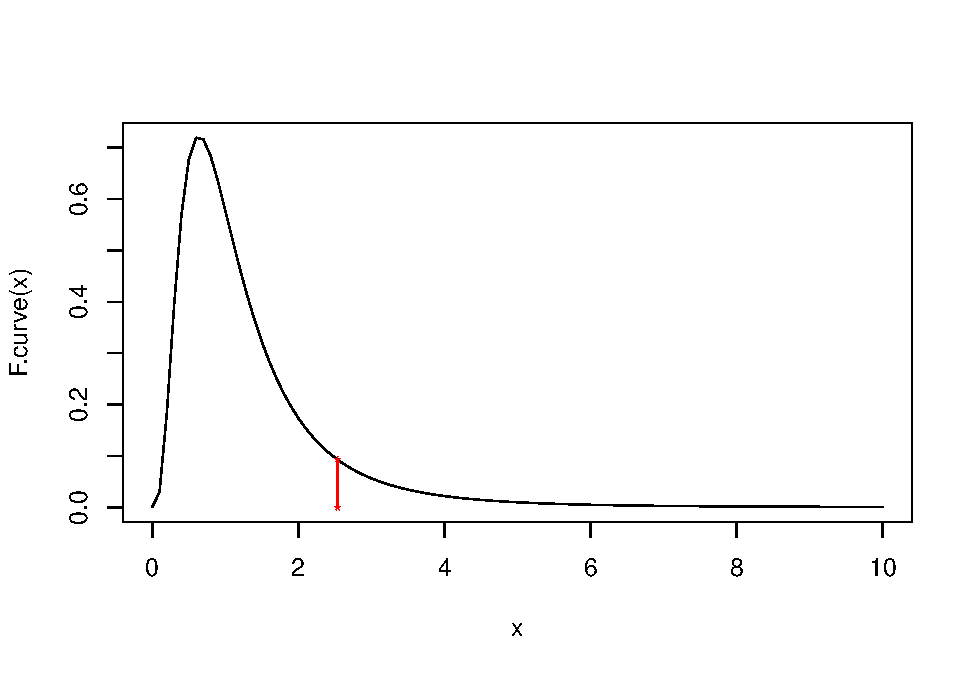
\includegraphics{13-Hypothesis-Testing_files/figure-latex/unnamed-chunk-9-1.pdf}

\begin{Shaded}
\begin{Highlighting}[]
\DecValTok{1}\SpecialCharTok{{-}}\FunctionTok{pf}\NormalTok{(F, }\DecValTok{10}\NormalTok{, }\DecValTok{8}\NormalTok{)}
\end{Highlighting}
\end{Shaded}

\begin{verbatim}
## [1] 0.09989054
\end{verbatim}

\begin{Shaded}
\begin{Highlighting}[]
\DecValTok{2}\SpecialCharTok{*}\NormalTok{(}\DecValTok{1}\SpecialCharTok{{-}}\FunctionTok{pf}\NormalTok{(F, }\DecValTok{10}\NormalTok{, }\DecValTok{8}\NormalTok{))}
\end{Highlighting}
\end{Shaded}

\begin{verbatim}
## [1] 0.1997811
\end{verbatim}

\begin{Shaded}
\begin{Highlighting}[]
\FunctionTok{qf}\NormalTok{(}\FloatTok{0.09989054}\NormalTok{, }\DecValTok{10}\NormalTok{,}\DecValTok{8}\NormalTok{)}
\end{Highlighting}
\end{Shaded}

\begin{verbatim}
## [1] 0.4204884
\end{verbatim}

\begin{Shaded}
\begin{Highlighting}[]
\FunctionTok{curve}\NormalTok{(F.curve, }\DecValTok{0}\NormalTok{, }\DecValTok{10}\NormalTok{)}
\FunctionTok{points}\NormalTok{(F, }\FunctionTok{F.curve}\NormalTok{(F), }\AttributeTok{pch =} \StringTok{\textquotesingle{}*\textquotesingle{}}\NormalTok{, }\AttributeTok{col =} \StringTok{\textquotesingle{}red\textquotesingle{}}\NormalTok{)}
\FunctionTok{points}\NormalTok{(F, }\DecValTok{0}\NormalTok{, }\AttributeTok{pch =} \StringTok{\textquotesingle{}*\textquotesingle{}}\NormalTok{, }\AttributeTok{col =} \StringTok{\textquotesingle{}red\textquotesingle{}}\NormalTok{)}
\FunctionTok{lines}\NormalTok{(}\FunctionTok{c}\NormalTok{(F,F), }\FunctionTok{c}\NormalTok{(}\DecValTok{0}\NormalTok{,}\FunctionTok{F.curve}\NormalTok{(F)), }\AttributeTok{col =} \StringTok{\textquotesingle{}red\textquotesingle{}}\NormalTok{)}
\FunctionTok{lines}\NormalTok{(}\FunctionTok{c}\NormalTok{(}\FunctionTok{qf}\NormalTok{(}\FloatTok{0.09989054}\NormalTok{, }\DecValTok{10}\NormalTok{,}\DecValTok{8}\NormalTok{),}\FunctionTok{qf}\NormalTok{(}\FloatTok{0.09989054}\NormalTok{, }\DecValTok{10}\NormalTok{,}\DecValTok{8}\NormalTok{)), }\FunctionTok{c}\NormalTok{(}\DecValTok{0}\NormalTok{,}\FunctionTok{F.curve}\NormalTok{(}\FunctionTok{qf}\NormalTok{(}\FloatTok{0.09989054}\NormalTok{, }\DecValTok{10}\NormalTok{,}\DecValTok{8}\NormalTok{))), }\AttributeTok{col =} \StringTok{\textquotesingle{}red\textquotesingle{}}\NormalTok{)}
\end{Highlighting}
\end{Shaded}

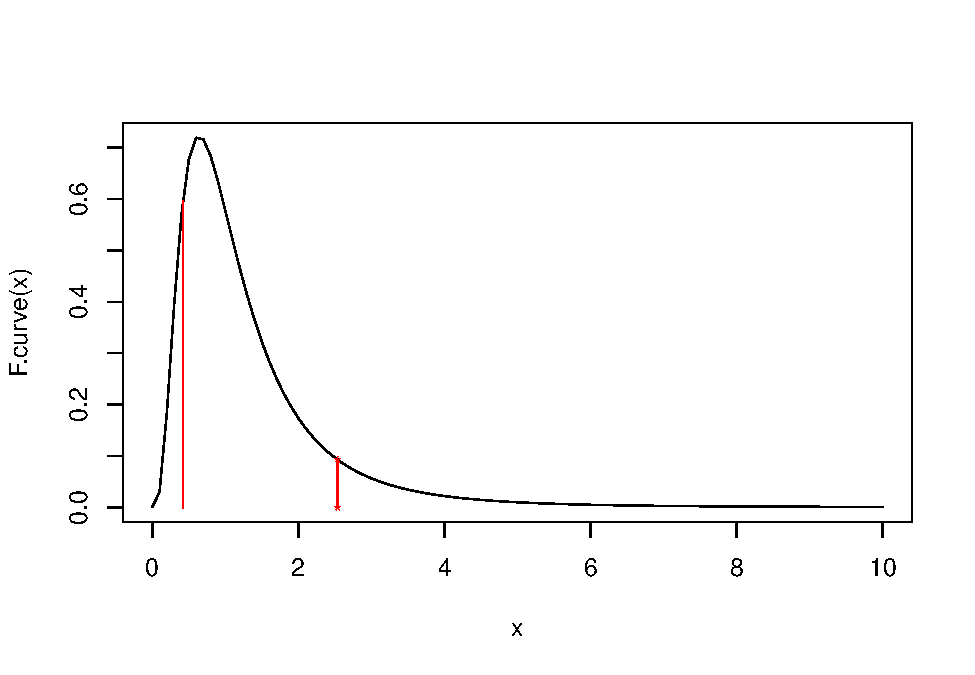
\includegraphics{13-Hypothesis-Testing_files/figure-latex/unnamed-chunk-9-2.pdf}

\begin{Shaded}
\begin{Highlighting}[]
\FunctionTok{curve}\NormalTok{(F.curve, }\DecValTok{0}\NormalTok{, }\DecValTok{10}\NormalTok{)}
\FunctionTok{lines}\NormalTok{(}\FunctionTok{c}\NormalTok{(}\FunctionTok{qf}\NormalTok{(}\FloatTok{0.025}\NormalTok{, }\DecValTok{10}\NormalTok{,}\DecValTok{8}\NormalTok{),}\FunctionTok{qf}\NormalTok{(}\FloatTok{0.025}\NormalTok{, }\DecValTok{10}\NormalTok{,}\DecValTok{8}\NormalTok{)), }\FunctionTok{c}\NormalTok{(}\DecValTok{0}\NormalTok{,}\FunctionTok{F.curve}\NormalTok{(}\FunctionTok{qf}\NormalTok{(}\FloatTok{0.025}\NormalTok{, }\DecValTok{10}\NormalTok{,}\DecValTok{8}\NormalTok{))), }\AttributeTok{col =} \StringTok{\textquotesingle{}blue\textquotesingle{}}\NormalTok{)}
\FunctionTok{lines}\NormalTok{(}\FunctionTok{c}\NormalTok{(}\FunctionTok{qf}\NormalTok{(}\FloatTok{0.975}\NormalTok{, }\DecValTok{10}\NormalTok{,}\DecValTok{8}\NormalTok{),}\FunctionTok{qf}\NormalTok{(}\FloatTok{0.975}\NormalTok{, }\DecValTok{10}\NormalTok{,}\DecValTok{8}\NormalTok{)), }\FunctionTok{c}\NormalTok{(}\DecValTok{0}\NormalTok{,}\FunctionTok{F.curve}\NormalTok{(}\FunctionTok{qf}\NormalTok{(}\FloatTok{0.975}\NormalTok{, }\DecValTok{10}\NormalTok{,}\DecValTok{8}\NormalTok{))), }\AttributeTok{col =} \StringTok{\textquotesingle{}blue\textquotesingle{}}\NormalTok{)}
\end{Highlighting}
\end{Shaded}

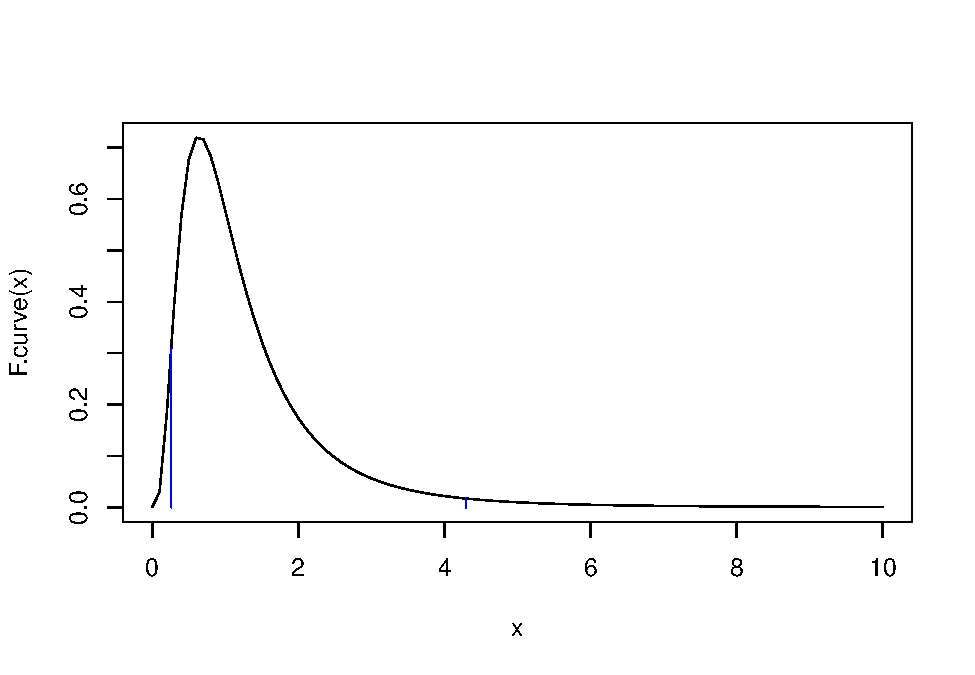
\includegraphics{13-Hypothesis-Testing_files/figure-latex/unnamed-chunk-9-3.pdf}

\hypertarget{likelihood-based-tests}{%
\section{Likelihood-based Tests}\label{likelihood-based-tests}}

In our discussions of point and interval estimation we found likelihood-based methods provided a general means of deriving estimators with (at least) good large-sample performance. The same is true with respect to testing. However, there's more than one way to use the likelihood function to define a test, and we'll discuss two strategies.

\hypertarget{wald-type-tests}{%
\subsection{Wald type tests}\label{wald-type-tests}}

Wald-type tests follow the strategy we've been using. The test is based on a point estimator and its distribution. The testing rule is essentially to reject the null if the point estimator sufficiently disagrees with the null where ``sufficiently'' is determined by the estimator's distribution. In the case of likelihood-based Wald tests the point estimator is the MLE and the distribution is the (asymptotic/approximate) normal distribution of the MLE. Therefore, all Wald-type likelihood-based tests of \(H_0:\theta = \theta_0\) versus \(H_a:\theta\ne \theta_0\) are of the form ``Reject \(H_0\) if:''
\[\theta_0 \notin (\hat\theta \pm z_{1-\alpha/2}[nI(\theta_0)]^{-1/2}),\]
because
\[\frac{\hat\theta - \theta_0}{[nI(\theta_0)]^{-1/2}}\stackrel{H_0}{\sim}N(0,1)\]
where \(\theta\) is a scalar.
Note: for point null tests \(H_0:\theta=\theta_0\) for \(p\times 1\) vector parameters \((\hat\theta-\theta_0)[nI(\theta_0)]^{-1/2}\) is a p-variate standard normal and the quadratic form \((\hat\theta-\theta_0)^{\top}[nI(\theta_0)]^{-1} (\hat\theta-\theta_0)\) has a Chi-squared distribution with \(p\) degrees of freedom. And, the Wald test is based on quantiles of this Chi-squared distribution.

Example: Suppose \(X_1, \ldots, X_n\) is a random sample from an Exponential distribution with scale parameter \(\lambda\) and consider testing \(H_0:\lambda \leq \lambda_0\) versus \(H_a:\lambda > \lambda_0\). The sample mean is the MLE of \(\lambda\), and \(n\overline X= \sum_{i=1}^nX_i \sim\) Gamma\((n, \lambda)\). Therefore, an exact test is based on the Gamma distribution, while a likelihood-based Wald test is based on \(\overline X \stackrel{H_0}{\sim}N(\lambda_0,\lambda_0^2/n)\), approximately. Suppose \(\lambda_0 = 5\) and we observe the following random sample of size 12:
\[x : 12.57,\,\,\,  1.83,\,\,\,  2.10,\,\,\,  3.00,\,\,\,  0.65,\,\,\,  2.74,\,\,\, 14.21,\,\,\,  1.72,\,\,\,  3.13,\,\,\,  1.63,\,\,\,  2.42,\,\,\,  9.33\]

\begin{Shaded}
\begin{Highlighting}[]
\NormalTok{x }\OtherTok{=} \FunctionTok{c}\NormalTok{(}\FloatTok{12.57}\NormalTok{,  }\FloatTok{1.83}\NormalTok{,  }\FloatTok{2.10}\NormalTok{,  }\FloatTok{3.00}\NormalTok{,  }\FloatTok{0.65}\NormalTok{,  }\FloatTok{2.74}\NormalTok{, }\FloatTok{14.21}\NormalTok{,  }\FloatTok{1.72}\NormalTok{,  }\FloatTok{3.13}\NormalTok{,  }\FloatTok{1.63}\NormalTok{,  }\FloatTok{2.42}\NormalTok{,  }\FloatTok{9.33}\NormalTok{)}
\NormalTok{xbar }\OtherTok{\textless{}{-}} \FunctionTok{mean}\NormalTok{(x)}
\NormalTok{xbar}
\end{Highlighting}
\end{Shaded}

\begin{verbatim}
## [1] 4.610833
\end{verbatim}

\begin{Shaded}
\begin{Highlighting}[]
\FunctionTok{c}\NormalTok{(xbar }\SpecialCharTok{{-}} \FloatTok{1.96}\SpecialCharTok{*}\DecValTok{5}\SpecialCharTok{/}\FunctionTok{sqrt}\NormalTok{(}\DecValTok{12}\NormalTok{), xbar }\SpecialCharTok{+} \FloatTok{1.96}\SpecialCharTok{*}\DecValTok{5}\SpecialCharTok{/}\FunctionTok{sqrt}\NormalTok{(}\DecValTok{12}\NormalTok{))}
\end{Highlighting}
\end{Shaded}

\begin{verbatim}
## [1] 1.781817 7.439850
\end{verbatim}

\begin{Shaded}
\begin{Highlighting}[]
\DecValTok{5}
\end{Highlighting}
\end{Shaded}

\begin{verbatim}
## [1] 5
\end{verbatim}

\begin{Shaded}
\begin{Highlighting}[]
\FunctionTok{c}\NormalTok{(}\FunctionTok{qgamma}\NormalTok{(}\FloatTok{0.025}\NormalTok{, }\AttributeTok{shape =} \DecValTok{12}\NormalTok{, }\AttributeTok{scale =} \DecValTok{5}\NormalTok{), }\FunctionTok{qgamma}\NormalTok{(}\FloatTok{0.975}\NormalTok{, }\AttributeTok{shape =} \DecValTok{12}\NormalTok{, }\AttributeTok{scale =} \DecValTok{5}\NormalTok{))}
\end{Highlighting}
\end{Shaded}

\begin{verbatim}
## [1] 31.00288 98.41019
\end{verbatim}

\begin{Shaded}
\begin{Highlighting}[]
\NormalTok{xbar }\SpecialCharTok{*} \DecValTok{12}
\end{Highlighting}
\end{Shaded}

\begin{verbatim}
## [1] 55.33
\end{verbatim}

\begin{Shaded}
\begin{Highlighting}[]
\FunctionTok{c}\NormalTok{(}\FunctionTok{qgamma}\NormalTok{(}\FloatTok{0.025}\NormalTok{, }\AttributeTok{shape =} \DecValTok{12}\NormalTok{, }\AttributeTok{scale =} \DecValTok{5}\NormalTok{), }\FunctionTok{qgamma}\NormalTok{(}\FloatTok{0.975}\NormalTok{, }\AttributeTok{shape =} \DecValTok{12}\NormalTok{, }\AttributeTok{scale =} \DecValTok{5}\NormalTok{))}\SpecialCharTok{/}\DecValTok{12}
\end{Highlighting}
\end{Shaded}

\begin{verbatim}
## [1] 2.583573 8.200849
\end{verbatim}

\begin{Shaded}
\begin{Highlighting}[]
\NormalTok{xbar}
\end{Highlighting}
\end{Shaded}

\begin{verbatim}
## [1] 4.610833
\end{verbatim}

Simulation of Type 1 error rates:

\begin{Shaded}
\begin{Highlighting}[]
\NormalTok{reps }\OtherTok{\textless{}{-}} \DecValTok{10000}
\NormalTok{errors }\OtherTok{\textless{}{-}} \FunctionTok{matrix}\NormalTok{(}\DecValTok{0}\NormalTok{, reps, }\DecValTok{2}\NormalTok{)}
\ControlFlowTok{for}\NormalTok{(r }\ControlFlowTok{in} \DecValTok{1}\SpecialCharTok{:}\NormalTok{reps)\{}
\NormalTok{  x }\OtherTok{\textless{}{-}} \FunctionTok{rexp}\NormalTok{(}\DecValTok{12}\NormalTok{,}\AttributeTok{rate =} \DecValTok{1}\SpecialCharTok{/}\DecValTok{5}\NormalTok{)}
\NormalTok{  xbar }\OtherTok{\textless{}{-}} \FunctionTok{mean}\NormalTok{(x)}
\NormalTok{  rr.wald }\OtherTok{\textless{}{-}} \FunctionTok{c}\NormalTok{(xbar }\SpecialCharTok{{-}} \FloatTok{1.96}\SpecialCharTok{*}\DecValTok{5}\SpecialCharTok{/}\FunctionTok{sqrt}\NormalTok{(}\DecValTok{12}\NormalTok{), xbar }\SpecialCharTok{+} \FloatTok{1.96}\SpecialCharTok{*}\DecValTok{5}\SpecialCharTok{/}\FunctionTok{sqrt}\NormalTok{(}\DecValTok{12}\NormalTok{))}
\NormalTok{  rr.exact }\OtherTok{\textless{}{-}} \FunctionTok{c}\NormalTok{(}\FunctionTok{qgamma}\NormalTok{(}\FloatTok{0.025}\NormalTok{, }\AttributeTok{shape =} \DecValTok{12}\NormalTok{, }\AttributeTok{scale =} \DecValTok{5}\NormalTok{), }\FunctionTok{qgamma}\NormalTok{(}\FloatTok{0.975}\NormalTok{, }\AttributeTok{shape =} \DecValTok{12}\NormalTok{, }\AttributeTok{scale =} \DecValTok{5}\NormalTok{))}\SpecialCharTok{/}\DecValTok{12}
\NormalTok{  errors[r, ] }\OtherTok{\textless{}{-}} \FunctionTok{c}\NormalTok{(}\FunctionTok{ifelse}\NormalTok{(}\DecValTok{5}\SpecialCharTok{\textgreater{}}\NormalTok{rr.wald[}\DecValTok{1}\NormalTok{] }\SpecialCharTok{\&} \DecValTok{5}\SpecialCharTok{\textless{}}\NormalTok{rr.wald[}\DecValTok{2}\NormalTok{],}\DecValTok{0}\NormalTok{,}\DecValTok{1}\NormalTok{), }\FunctionTok{ifelse}\NormalTok{(xbar}\SpecialCharTok{\textgreater{}}\NormalTok{rr.exact[}\DecValTok{1}\NormalTok{] }\SpecialCharTok{\&}\NormalTok{ xbar}\SpecialCharTok{\textless{}}\NormalTok{rr.exact[}\DecValTok{2}\NormalTok{],}\DecValTok{0}\NormalTok{,}\DecValTok{1}\NormalTok{))}
\NormalTok{\}}
\FunctionTok{colMeans}\NormalTok{(errors)}
\end{Highlighting}
\end{Shaded}

\begin{verbatim}
## [1] 0.0487 0.0536
\end{verbatim}

\hypertarget{likelihood-ratio-tests}{%
\subsection{Likelihood ratio tests}\label{likelihood-ratio-tests}}

Likelihood ratio tests (LRTs) operate a little differently compared to Wald tests. The LRT idea is that parameter values with corresponding likelihood values near the maximum are plausible, while those with low likelihood values are implausible. For testing \(H_0:\theta = \theta_0\) versus \(H_a:\theta\ne \theta_0\) this means if \(\frac{L(\theta_0)}{L(\hat\theta)}\) is close to 1 the null is supported while if the ratio is close to zero the alternative is supported. How ``close'' is close again depends on the null-hypothesis distribution of the likelihood ratio. A general asymptotic result holds that for scalar parameters
\[-2[\ell(\theta_0) - \ell(\hat\theta)] \stackrel{H_0}{\sim} Chi-squared(1)\]
approximately. This result also holds for general composite hypotheses \(H_0:\theta\in \Theta_0\) versus \(H_a: \theta\in \Theta \cap \Theta_0^c\) so that
\[-2[\sup_{\theta\in \Theta_0}\{\ell(\theta)\} - \ell(\hat\theta)]\stackrel{H_0}{\sim} Chi-squared(df)\]
where \(df\) is equal to the difference in dimensions of the parameter space.

Example: Consider a test for \(H_0:\mu = \mu_0\) versus \(H_a:\mu \ne \mu_0\) for a normal population with unknown variance. In that case \(\Theta\) is the two-dimensional parameter space for \((\mu, \sigma^2)\) which is \(\mathbb{R}\times \mathbb{R}^+\) and \(\Theta_0\) is the one-dimensional subspace \(\{\mu_0\}\times \mathbb{R}^+\). The unrestricted MLEs are \(\overline x\) and \(\hat\sigma^2 = n^{-1}\sum_{i=1}^n(x_i - \overline x)^2\). It's not hard to show the restriced MLE for \(\sigma^2\) under the null hypothesis is \(\hat\sigma_0^2 = n^{-1}\sum_{i=1}^n (x_i - \mu_0)^2\). To test \(H_0\) we compute the test statistic
\[\Lambda := -2[\ell(\mu_0, \hat\sigma_0^2) - \ell(\overline x, \hat\sigma^2)]\]
and reject the null hypothesis if \(\Lambda > \chi^2_{1-\alpha}(1)\), the \(1-\alpha\) lower quantile of the Chi squared distribution with 1 degree of freedom. Let's perform the test given the following sample:

\begin{Shaded}
\begin{Highlighting}[]
\NormalTok{x }\OtherTok{\textless{}{-}} \FunctionTok{rnorm}\NormalTok{(}\DecValTok{22}\NormalTok{, }\DecValTok{8}\NormalTok{, }\DecValTok{6}\NormalTok{)}
\NormalTok{x}
\end{Highlighting}
\end{Shaded}

\begin{verbatim}
##  [1]  4.0634008  9.1198213 13.6167056  7.1889954 13.9577182 10.2795735
##  [7]  7.8406222  6.1487191  0.2090839  0.7775581 10.5912890 10.3346847
## [13] 19.6868480  0.8674458 12.9657995  8.1965838  2.9815080  7.5730705
## [19]  8.2187202  2.9247010  4.4469792  3.5998290
\end{verbatim}

\begin{Shaded}
\begin{Highlighting}[]
\NormalTok{xbar }\OtherTok{\textless{}{-}} \FunctionTok{mean}\NormalTok{(x)}
\NormalTok{xbar}
\end{Highlighting}
\end{Shaded}

\begin{verbatim}
## [1] 7.526803
\end{verbatim}

\begin{Shaded}
\begin{Highlighting}[]
\NormalTok{mu0 }\OtherTok{\textless{}{-}} \DecValTok{7}
\NormalTok{mle }\OtherTok{\textless{}{-}}\NormalTok{ (}\DecValTok{1}\SpecialCharTok{/}\DecValTok{22}\NormalTok{)}\SpecialCharTok{*}\FunctionTok{sum}\NormalTok{((x}\SpecialCharTok{{-}}\NormalTok{xbar)}\SpecialCharTok{\^{}}\DecValTok{2}\NormalTok{)}
\NormalTok{mle}
\end{Highlighting}
\end{Shaded}

\begin{verbatim}
## [1] 23.11427
\end{verbatim}

\begin{Shaded}
\begin{Highlighting}[]
\NormalTok{mle0 }\OtherTok{\textless{}{-}}\NormalTok{ (}\DecValTok{1}\SpecialCharTok{/}\DecValTok{22}\NormalTok{)}\SpecialCharTok{*}\FunctionTok{sum}\NormalTok{((x }\SpecialCharTok{{-}}\NormalTok{ mu0)}\SpecialCharTok{\^{}}\DecValTok{2}\NormalTok{)}
\NormalTok{mle0}
\end{Highlighting}
\end{Shaded}

\begin{verbatim}
## [1] 23.39179
\end{verbatim}

\begin{Shaded}
\begin{Highlighting}[]
\NormalTok{loglhood }\OtherTok{\textless{}{-}} \ControlFlowTok{function}\NormalTok{(mu, sigma2)  }\FunctionTok{sum}\NormalTok{(}\FunctionTok{dnorm}\NormalTok{(x,mu,}\FunctionTok{sqrt}\NormalTok{(sigma2),}\AttributeTok{log =} \ConstantTok{TRUE}\NormalTok{))}
\NormalTok{Lambda }\OtherTok{\textless{}{-}}\NormalTok{ (}\SpecialCharTok{{-}}\DecValTok{2}\NormalTok{)}\SpecialCharTok{*}\NormalTok{(}\FunctionTok{loglhood}\NormalTok{(mu0,mle0) }\SpecialCharTok{{-}} \FunctionTok{loglhood}\NormalTok{(xbar,mle)) }
\NormalTok{Lambda}
\end{Highlighting}
\end{Shaded}

\begin{verbatim}
## [1] 0.2625694
\end{verbatim}

\begin{Shaded}
\begin{Highlighting}[]
\FunctionTok{qchisq}\NormalTok{(}\FloatTok{0.95}\NormalTok{, }\DecValTok{1}\NormalTok{)}
\end{Highlighting}
\end{Shaded}

\begin{verbatim}
## [1] 3.841459
\end{verbatim}

Example: Consider the following data on cell phone battery charge times
\[8.0, \,\,\, 8.1, \,\,\, 8.9, \,\,\, 9.1, \,\,\, 9.2, \,\,\, 9.3, \,\,\, 9.4, \,\,\, 9.4\]
Assuming these times constitute a random sample from a normal population test the hypothesis \(H_0:\sigma^2 \leq 0.2\) versus \(H_a:\sigma^2 > 0.2\) using an LRT at \(\alpha = 0.05\).
The loglikelihood, again, is
\[\ell(\mu, \sigma^2; x) = -(n/2)\log [2\pi\sigma^2] - \frac{1}{2\sigma^2}\sum_{i=1}^n(x_i - \mu)^2.\]
The unrestricted MLEs are \(\overline x = 8.925\) and \(\hat\sigma^2 = 0.28\). Under the null hypothesis the MLE of \(\mu\) remains \(\overline x = 8.925\) because the derivative of the loglikelihood w.r.t. \(\mu\) is proportional to \(\sigma^2\); i.e., it equals \(\frac{1}{\sigma^2}\sum_{i=1}^n (x_i - \mu)\). Then, setting equal to zero we see the MLE for \(\mu\) is still \(\overline x\). To find the restricted MLE of \(\sigma^2\) under \(H_0\), plot the loglikelihood as a function of \(\sigma^2\) with \(\mu = \overline x\) below and note that it is maximized at \(0.2\) over the set \(\sigma^2 \leq 0.2\). The test statistic is
\[-2(\ell(8.925,0.2;x) - \ell(8.925,0.28;x)) = 0.501\]
which is below the cutoff of 3.84, the \(95\%\) quantile of the Chi-squared distribution with 1 degree of freedom (the difference in two versus one free parameter in the alternative versus null hypothesis).

\begin{Shaded}
\begin{Highlighting}[]
\NormalTok{x }\OtherTok{\textless{}{-}} \FunctionTok{c}\NormalTok{(}\FloatTok{8.0}\NormalTok{,}\FloatTok{8.1}\NormalTok{,}\FloatTok{8.9}\NormalTok{,}\FloatTok{9.1}\NormalTok{,}\FloatTok{9.2}\NormalTok{,}\FloatTok{9.3}\NormalTok{,}\FloatTok{9.4}\NormalTok{,}\FloatTok{9.4}\NormalTok{)}
\NormalTok{ell }\OtherTok{\textless{}{-}} \ControlFlowTok{function}\NormalTok{(sig2) }\FunctionTok{sum}\NormalTok{(}\FunctionTok{dnorm}\NormalTok{(x,}\FunctionTok{mean}\NormalTok{(x),}\FunctionTok{sqrt}\NormalTok{(sig2),}\AttributeTok{log =} \ConstantTok{TRUE}\NormalTok{))}
\NormalTok{app.ell }\OtherTok{\textless{}{-}} \ControlFlowTok{function}\NormalTok{(sig2) }\FunctionTok{apply}\NormalTok{(}\FunctionTok{matrix}\NormalTok{(sig2,}\FunctionTok{length}\NormalTok{(sig2),}\DecValTok{1}\NormalTok{),}\DecValTok{1}\NormalTok{,ell)}
\FunctionTok{curve}\NormalTok{(app.ell,}\DecValTok{0}\NormalTok{,}\DecValTok{2}\NormalTok{)  }
\FunctionTok{abline}\NormalTok{(}\AttributeTok{v =} \FloatTok{0.2}\NormalTok{, }\AttributeTok{col =} \StringTok{\textquotesingle{}red\textquotesingle{}}\NormalTok{)}
\end{Highlighting}
\end{Shaded}

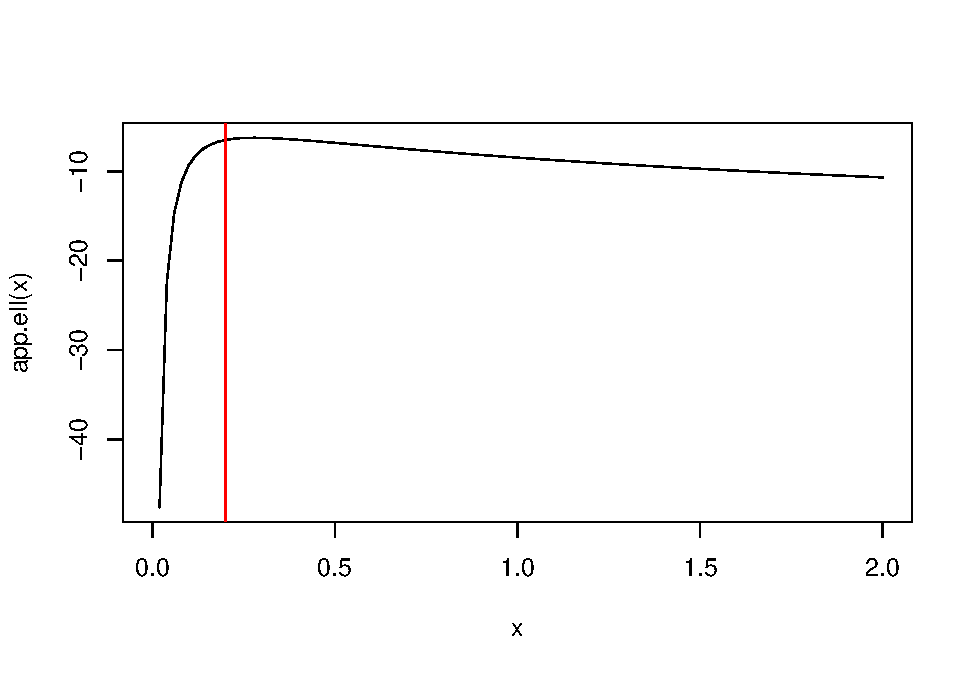
\includegraphics{13-Hypothesis-Testing_files/figure-latex/unnamed-chunk-13-1.pdf}

\begin{Shaded}
\begin{Highlighting}[]
\NormalTok{test.stat }\OtherTok{\textless{}{-}} \SpecialCharTok{{-}}\DecValTok{2}\SpecialCharTok{*}\NormalTok{(}\FunctionTok{ell}\NormalTok{(}\FloatTok{0.2}\NormalTok{)}\SpecialCharTok{{-}}\FunctionTok{ell}\NormalTok{(}\FloatTok{0.28}\NormalTok{))}
\NormalTok{test.stat}
\end{Highlighting}
\end{Shaded}

\begin{verbatim}
## [1] 0.5010792
\end{verbatim}

\begin{Shaded}
\begin{Highlighting}[]
\FunctionTok{qchisq}\NormalTok{(}\FloatTok{0.95}\NormalTok{,}\DecValTok{1}\NormalTok{)}
\end{Highlighting}
\end{Shaded}

\begin{verbatim}
## [1] 3.841459
\end{verbatim}

\hypertarget{chi-squared-tests-for-tabulated-data}{%
\section{Chi Squared tests for tabulated data}\label{chi-squared-tests-for-tabulated-data}}

To this point most of our experiments have dealt with continuous data. But, a common type of data encountered in experiments is tabulated or cross-classified data. For example, consider the following data on phsychologists' opinions concerning the causes of schizophrenia:

\begin{longtable}[]{@{}ccccc@{}}
\toprule()
& & Origin & & \\
\midrule()
\endhead
School & Biogenic & Environment & Combination & \\
Eclectic & 90 & 12 & 78 & 180 \\
Medical & 13 & 1 & 6 & 20 \\
Psychoanalytic & 19 & 13 & 50 & 82 \\
& 122 & 26 & 134 & 282 \\
\bottomrule()
\end{longtable}

A test of interest is whether the psychologists' schools of thought are related to their responses. Statistically, this can be interpreted as a test of independence between the variables ``school'' and ``cause''. A test of this hypothesis of independence may be based on a multinomial sampling distribution where the 282 respondents are assumed to be a random sample from a multinomial distribution with 9 cross-classified categories based on ``school'' and ``cause''. This distribution has 8 free parameters for the category memberships. Under the null hypothesis, the joint probabilities are products of the marginal ``school'' and ``cause'' probabilities, so that there are only 4 free parameters.

A Chi-squared test for independence is based on the following test statistic:
\[\chi^2 = \sum_{i=1}^I (O_i - E_i)^2 / E_i\]
where \(O_i\) is the observed category count and \(E_i\) is the expected category count under \(H_0\). Under the hypothesis of independence we expect the category counts to be \(n = 282\) times the products of marginal category probabilities. For example, we expect to find \(282 *(180/282)*(122/282) = 77.87\) counts in the Biogenic-Eclectic category; we observe 90. Similarly, we expect \(26*20/282 = 1.84\) counts in the Medical-Environment category; we observe 1. The first summand in the test statistic is \((77.87 - 90)^2 / 77.87 = 1.88952\). Following along this way, we compute the test statistic to be \(\chi^2 = 22.37769\). The \(chi^2\) test statistic is approximately Chi-squared distributed with df equal to the difference in the number of free parameters in \(H_0\) and \(H_a\). In this case, that is \(8 - 4 = 4\). Since the \(95\%\) quantile of the Chi-squared distribution with 4 df is 9.487729, we reject the null hypothesis of independence.
We could also perform an LRT of the independence hypothesis based on the multinomial distribution of the cell counts. The MLEs of the cell proportions are simply the observed cell proportions. The multinomial loglikelihood is given by
\[\ell(p;x_1, \ldots, x_n) = \log \frac{n!}{x_1!\times \cdots \times x_9!} + \sum_{j=1}^9 x_j\log p_j.\]
In R, we can simply use ``dmultinom'' with option log = TRUE to compute the loglikleihood.

\begin{Shaded}
\begin{Highlighting}[]
\NormalTok{test.stat }\OtherTok{\textless{}{-}} \SpecialCharTok{{-}}\DecValTok{2}\SpecialCharTok{*}\NormalTok{(}\FunctionTok{dmultinom}\NormalTok{(}\FunctionTok{c}\NormalTok{(}\DecValTok{90}\NormalTok{,}\DecValTok{12}\NormalTok{,}\DecValTok{78}\NormalTok{,}\DecValTok{13}\NormalTok{,}\DecValTok{1}\NormalTok{,}\DecValTok{6}\NormalTok{,}\DecValTok{19}\NormalTok{,}\DecValTok{13}\NormalTok{,}\DecValTok{50}\NormalTok{),}\AttributeTok{prob =} \FunctionTok{c}\NormalTok{(}\DecValTok{180}\SpecialCharTok{*}\DecValTok{122}\NormalTok{, }\DecValTok{180}\SpecialCharTok{*}\DecValTok{26}\NormalTok{, }\DecValTok{180}\SpecialCharTok{*}\DecValTok{134}\NormalTok{, }\DecValTok{20}\SpecialCharTok{*}\DecValTok{122}\NormalTok{, }\DecValTok{20}\SpecialCharTok{*}\DecValTok{26}\NormalTok{, }\DecValTok{20}\SpecialCharTok{*}\DecValTok{134}\NormalTok{, }\DecValTok{82}\SpecialCharTok{*}\DecValTok{122}\NormalTok{, }\DecValTok{82}\SpecialCharTok{*}\DecValTok{26}\NormalTok{, }\DecValTok{82}\SpecialCharTok{*}\DecValTok{134}\NormalTok{)}\SpecialCharTok{/}\NormalTok{(}\DecValTok{282}\SpecialCharTok{*}\DecValTok{282}\NormalTok{), }\AttributeTok{log =} \ConstantTok{TRUE}\NormalTok{)}\SpecialCharTok{{-}}\FunctionTok{dmultinom}\NormalTok{(}\FunctionTok{c}\NormalTok{(}\DecValTok{90}\NormalTok{,}\DecValTok{12}\NormalTok{,}\DecValTok{78}\NormalTok{,}\DecValTok{13}\NormalTok{,}\DecValTok{1}\NormalTok{,}\DecValTok{6}\NormalTok{,}\DecValTok{19}\NormalTok{,}\DecValTok{13}\NormalTok{,}\DecValTok{50}\NormalTok{),}\AttributeTok{prob =} \FunctionTok{c}\NormalTok{(}\DecValTok{90}\NormalTok{,}\DecValTok{12}\NormalTok{,}\DecValTok{78}\NormalTok{,}\DecValTok{13}\NormalTok{,}\DecValTok{1}\NormalTok{,}\DecValTok{6}\NormalTok{,}\DecValTok{19}\NormalTok{,}\DecValTok{13}\NormalTok{,}\DecValTok{50}\NormalTok{)}\SpecialCharTok{/}\DecValTok{282}\NormalTok{, }\AttributeTok{log =} \ConstantTok{TRUE}\NormalTok{))}
\NormalTok{test.stat}
\end{Highlighting}
\end{Shaded}

\begin{verbatim}
## [1] 23.03619
\end{verbatim}

\begin{Shaded}
\begin{Highlighting}[]
\FunctionTok{qchisq}\NormalTok{(}\FloatTok{0.95}\NormalTok{,}\DecValTok{4}\NormalTok{)}
\end{Highlighting}
\end{Shaded}

\begin{verbatim}
## [1] 9.487729
\end{verbatim}

For completeness, let's show the MLEs of multinomial cell probabilities are the corresponding sample proportions. The loglikelihood is equal to
\[\ell(p;x) = \log \left(\frac{n!}{x_1!\times x_2!\times \cdots\times x_9!} + x_1\log(p_1) \times \cdots \times x_8 \log(p_8) + (n-x_1-x_2-\cdots -x_8)\log(1-p_1-\cdots -p_8)\right).\]
Take the derivative of the loglikelihood w.r.t. \(p_1\), set equal to zero, and find
\[\frac{1 - p_1 - p_2 - \cdots - p_8}{p_1} - \frac{n-x_1-x_2-\cdots -x_8}{x_1}\]
Divide the right-hand-side by \(n\) in both the numerator and denominator to find
\[\frac{1 - p_1 - p_2 - \cdots - p_8}{p_1} = \frac{1-\frac{x_1}{n} - \frac{x_2}{n}-\cdots - \frac{x_8}{n}}{\frac{x_1}{n}}.\]
That this holds simultaneously for derivatives with respect to \(p_2\) through \(p_8\) implies the MLEs of the cell probabilitites are exactly the sample cell proportions. A similar argument can be made under \(H_0\) to show the MLEs under \(H_0\) are the sample marginal cell proportions.

\hypertarget{goodness-of-fit-tests}{%
\subsection{Goodness of fit tests}\label{goodness-of-fit-tests}}

The same Chi-squared test used above comparing observed awith expected cell counts is used to test the ``goodness of fit'' of a model to a data set. This test is most often used with discrete data, but can be used with continuous data by ``binning'' or discretizing continuous data in the same fashion as a histogram. For tabulated data the goodness of fit test statistic has df \(k-p-1\) where \(k\) is the number of cells in the table and \(p\) is the number of estimated parameters in the null hypothesis.

Example: Suppose an experiment records the number of customers entering a salon each hour during a weekday for the purpose of determining staffing requirements. The observed data are as follows:

\begin{longtable}[]{@{}lllllllllll@{}}
\toprule()
8am & 9am & 10am & 11am & 12pm & 1pm & 2pm & 3pm & 4pm & 5pm & 6pm \\
\midrule()
\endhead
3 & 6 & 14 & 11 & 6 & 4 & 4 & 3 & 8 & 11 & 3 \\
\bottomrule()
\end{longtable}

We decide to perform a goodness of fit test to determine whether the data fit a Poisson distribution. It the data appear to be a Poisson random sample, then that implies there is not a strong temporal pattern in the data. On the other hand if the data do not fit a Poisson distribution the lack of fit may be caused by a temporal pattern (so that the data are not iid). Based on the computation below, we see we reject the null hypothesis that the data are a Poisson random sample at \(\alpha\) level \(5\%\).

Below we bin the data into categories of 0-3 counts, 4-7 counts, 8-11, and 12+. A good rule of thumb is to choose bins such that the expected counts are not less than 5.

\begin{Shaded}
\begin{Highlighting}[]
\NormalTok{x }\OtherTok{\textless{}{-}} \FunctionTok{c}\NormalTok{(}\DecValTok{3}\NormalTok{,}\DecValTok{6}\NormalTok{,}\DecValTok{14}\NormalTok{,}\DecValTok{11}\NormalTok{,}\DecValTok{6}\NormalTok{,}\DecValTok{4}\NormalTok{,}\DecValTok{4}\NormalTok{,}\DecValTok{3}\NormalTok{,}\DecValTok{8}\NormalTok{,}\DecValTok{11}\NormalTok{,}\DecValTok{3}\NormalTok{)}
\NormalTok{n }\OtherTok{\textless{}{-}} \DecValTok{11}
\NormalTok{bins }\OtherTok{\textless{}{-}} \FunctionTok{c}\NormalTok{(}\DecValTok{3}\NormalTok{,}\DecValTok{4}\NormalTok{,}\DecValTok{3}\NormalTok{,}\DecValTok{1}\NormalTok{)}
\NormalTok{eis }\OtherTok{\textless{}{-}}\NormalTok{ n}\SpecialCharTok{*}\FunctionTok{c}\NormalTok{(}\FunctionTok{sum}\NormalTok{(}\FunctionTok{dpois}\NormalTok{(}\DecValTok{0}\SpecialCharTok{:}\DecValTok{3}\NormalTok{, }\FunctionTok{mean}\NormalTok{(x))),}\FunctionTok{sum}\NormalTok{(}\FunctionTok{dpois}\NormalTok{(}\DecValTok{4}\SpecialCharTok{:}\DecValTok{7}\NormalTok{, }\FunctionTok{mean}\NormalTok{(x))),}\FunctionTok{sum}\NormalTok{(}\FunctionTok{dpois}\NormalTok{(}\DecValTok{8}\SpecialCharTok{:}\DecValTok{11}\NormalTok{, }\FunctionTok{mean}\NormalTok{(x))),   }\DecValTok{1}\SpecialCharTok{{-}}\FunctionTok{ppois}\NormalTok{(}\DecValTok{11}\NormalTok{,}\FunctionTok{mean}\NormalTok{(x)))}
\FunctionTok{sum}\NormalTok{(((bins }\SpecialCharTok{{-}}\NormalTok{ eis)}\SpecialCharTok{\^{}}\DecValTok{2}\NormalTok{)}\SpecialCharTok{/}\NormalTok{eis)}
\end{Highlighting}
\end{Shaded}

\begin{verbatim}
## [1] 4.610001
\end{verbatim}

\begin{Shaded}
\begin{Highlighting}[]
\FunctionTok{qchisq}\NormalTok{(}\FloatTok{0.95}\NormalTok{,}\DecValTok{4{-}1{-}1}\NormalTok{)}
\end{Highlighting}
\end{Shaded}

\begin{verbatim}
## [1] 5.991465
\end{verbatim}

\begin{Shaded}
\begin{Highlighting}[]
\DecValTok{1}\SpecialCharTok{{-}}\FunctionTok{pchisq}\NormalTok{(}\FunctionTok{sum}\NormalTok{(((bins }\SpecialCharTok{{-}}\NormalTok{ eis)}\SpecialCharTok{\^{}}\DecValTok{2}\NormalTok{)}\SpecialCharTok{/}\NormalTok{eis),}\DecValTok{4{-}1{-}1}\NormalTok{)}
\end{Highlighting}
\end{Shaded}

\begin{verbatim}
## [1] 0.09975877
\end{verbatim}

\hypertarget{anova}{%
\chapter{ANOVA}\label{anova}}

One of the most important experiments we've discussed in the course involves the comparison of two populations in terms of their means. This kind of comparison motivated our study of the two-sample t-test and CI for the difference of two population means. These are very useful statistical methods, but why stop at comparing two populations? Often, we would like to compare three or more populations. For example, suppose a company marketing laundry detergent wants to compare 4 product designs (the detergent container and its labeling) in a pilot study. Using t-tests or CIs we could make pairwise comparisons (there are 4 choose 2, or, 6 pf these) but this causes some issues. Specifically, suppose there are no difference in the product designs and suppose we conduct 6 pairwise \(t\) tests at \(\alpha = 0.05\). If the 6 tests are independent (the test statistics are mutually independen r.v.'s) then the chance we make at least 1 Type 1 error is \(1-0.95^6 = 0.265\)! Even if there are no deifferences, there's a good chance we'll find at least one difference by chance alone. In order to avoid the Type 1 error inflation caused by \emph{multiple testing} one strategy---called Bonferroni correction---requires that we conduct each test at level \(\alpha / 6 = 0.00833\) so that the \emph{family-wise} Type 1 error rate is no more than \(1-(1-0.00833)^6 = 0.041 \leq 0.05\). This fixes our Type 1 error inflation problem, but it also means our power to detect fale null hypotheses (detect differences in response for different product designs) is severely hampered. Can we do better? Fortunately, the answer is yes! The alternative, improved strategy for comparing multiple population means is called ANOVA (analysis of variance) and its the focus of this section.

\hypertarget{analysis-of-variance}{%
\section{Analysis of variance}\label{analysis-of-variance}}

The general setup is as follows: we conduct an experiment in which we observe a random sample of size \(n\) from each of \(J\) populations so that the total sample size is \(N=nJ\). Denote the samples by \(X_{ij}\) for individual \(i=1, \ldots, n\) in the sample from population \(j=1,\ldots, J\). (It's possible, of course, to consider random samples of different sizes, but for simplicity we consider only the \emph{balanced} case). Our goal in this experiemnt is to evaluate the null hypothesis \(H_0: \mu_j = \mu\) for all \(j = 1,\ldots, J\), meaning that all the populations have the same mean. Further, we assume populations are normal with equal variance; this means that the populations are, essentially, equivalent under \(H_0\). The alternative hypothesis is that at least one population mean differs from the others.

Rather than comparing sample means to evaluate \(H_0\) we (somewhat counterintuitively) compare two estimators of the population variance. Consider the following decomposition:

\[\sum_{i=1}^n\sum_{j=1}^J(X_{ij} - \overline X)^2 = \sum_{i=1}^n\sum_{j=1}^J (X_{ij} - \overline X_j)^2 + n\sum_{j=1}^J (\overline X_j - \overline X)^2.\]
The left hand side of the equals sign in the above display is called the total sum of squares TSS and it decomposes into the sum of the error sum of squares ESS (or residual sum of squares) and the treatment sum of squares TrSS. Under the null hypothesis all three of these sums of squares can be used to estimate \(\sigma^2\), the common variance among the \(J\) populations. Further, the error sum of squares and treatment sum of squares are independent and satisfy
\[\frac{TrSS}{ESS} \stackrel{H_0}{\sim}F(J-1, J(n-1)).\]
The ANOVA F-test rejects the null hypothesis of equality of group means if \(F = TrSS/ESS\) is more extreme than the upper \(1-\alpha\) quantile of the F distribution with df \(J-1\) and \(J(n-1)\).

\hypertarget{crop-data-in-depth-example}{%
\section{Crop data in-depth example}\label{crop-data-in-depth-example}}

The embedded data comes from an experiment examining the effects of three types of fertilizer on crop yield. According to the data below there are 96 observations of yield, 32 each from each fertilizer type. And, the mean yields for the three fertilizer types are all very close to 177.

\begin{Shaded}
\begin{Highlighting}[]
\NormalTok{crops }\OtherTok{\textless{}{-}} \FunctionTok{read.csv}\NormalTok{(}\StringTok{"crop.data.csv"}\NormalTok{, }\AttributeTok{header =} \ConstantTok{TRUE}\NormalTok{, }\AttributeTok{colClasses =} \FunctionTok{c}\NormalTok{(}\StringTok{"factor"}\NormalTok{, }\StringTok{"factor"}\NormalTok{, }\StringTok{"factor"}\NormalTok{, }\StringTok{"numeric"}\NormalTok{))}
\NormalTok{m }\OtherTok{\textless{}{-}} \FunctionTok{mean}\NormalTok{(crops}\SpecialCharTok{$}\NormalTok{yield)}
\NormalTok{m1 }\OtherTok{\textless{}{-}} \FunctionTok{mean}\NormalTok{(crops}\SpecialCharTok{$}\NormalTok{yield[crops}\SpecialCharTok{$}\NormalTok{fertilizer }\SpecialCharTok{==} \DecValTok{1}\NormalTok{])}
\NormalTok{m2 }\OtherTok{\textless{}{-}} \FunctionTok{mean}\NormalTok{(crops}\SpecialCharTok{$}\NormalTok{yield[crops}\SpecialCharTok{$}\NormalTok{fertilizer }\SpecialCharTok{==} \DecValTok{2}\NormalTok{])}
\NormalTok{m3 }\OtherTok{\textless{}{-}} \FunctionTok{mean}\NormalTok{(crops}\SpecialCharTok{$}\NormalTok{yield[crops}\SpecialCharTok{$}\NormalTok{fertilizer }\SpecialCharTok{==} \DecValTok{3}\NormalTok{])}

\NormalTok{m}
\end{Highlighting}
\end{Shaded}

\begin{verbatim}
## [1] 177.0155
\end{verbatim}

\begin{Shaded}
\begin{Highlighting}[]
\NormalTok{m1}
\end{Highlighting}
\end{Shaded}

\begin{verbatim}
## [1] 176.757
\end{verbatim}

\begin{Shaded}
\begin{Highlighting}[]
\NormalTok{m2}
\end{Highlighting}
\end{Shaded}

\begin{verbatim}
## [1] 176.9332
\end{verbatim}

\begin{Shaded}
\begin{Highlighting}[]
\NormalTok{m3}
\end{Highlighting}
\end{Shaded}

\begin{verbatim}
## [1] 177.3562
\end{verbatim}

\begin{Shaded}
\begin{Highlighting}[]
\FunctionTok{length}\NormalTok{(crops}\SpecialCharTok{$}\NormalTok{yield)}
\end{Highlighting}
\end{Shaded}

\begin{verbatim}
## [1] 96
\end{verbatim}

\begin{Shaded}
\begin{Highlighting}[]
\FunctionTok{sum}\NormalTok{(crops}\SpecialCharTok{$}\NormalTok{fertilizer }\SpecialCharTok{==} \DecValTok{1}\NormalTok{)}
\end{Highlighting}
\end{Shaded}

\begin{verbatim}
## [1] 32
\end{verbatim}

\begin{Shaded}
\begin{Highlighting}[]
\FunctionTok{sum}\NormalTok{(crops}\SpecialCharTok{$}\NormalTok{fertilizer }\SpecialCharTok{==} \DecValTok{2}\NormalTok{)}
\end{Highlighting}
\end{Shaded}

\begin{verbatim}
## [1] 32
\end{verbatim}

\begin{Shaded}
\begin{Highlighting}[]
\FunctionTok{sum}\NormalTok{(crops}\SpecialCharTok{$}\NormalTok{fertilizer }\SpecialCharTok{==} \DecValTok{3}\NormalTok{)}
\end{Highlighting}
\end{Shaded}

\begin{verbatim}
## [1] 32
\end{verbatim}

We can compute the ANOVA F-test ``by hand'' in R by computing the component sums of squares and comparing to the appropriate lower and upper F quantiles using the qf function or by computing the p-value.

\begin{Shaded}
\begin{Highlighting}[]
\CommentTok{\# SSE}

\NormalTok{SSE }\OtherTok{\textless{}{-}} \FunctionTok{sum}\NormalTok{((crops}\SpecialCharTok{$}\NormalTok{yield[crops}\SpecialCharTok{$}\NormalTok{fertilizer }\SpecialCharTok{==} \DecValTok{1}\NormalTok{] }\SpecialCharTok{{-}}\NormalTok{ m1)}\SpecialCharTok{\^{}}\DecValTok{2}\NormalTok{)}\SpecialCharTok{+}\FunctionTok{sum}\NormalTok{((crops}\SpecialCharTok{$}\NormalTok{yield[crops}\SpecialCharTok{$}\NormalTok{fertilizer }\SpecialCharTok{==} \DecValTok{2}\NormalTok{] }\SpecialCharTok{{-}}\NormalTok{ m2)}\SpecialCharTok{\^{}}\DecValTok{2}\NormalTok{)}\SpecialCharTok{+}\FunctionTok{sum}\NormalTok{((crops}\SpecialCharTok{$}\NormalTok{yield[crops}\SpecialCharTok{$}\NormalTok{fertilizer }\SpecialCharTok{==} \DecValTok{3}\NormalTok{] }\SpecialCharTok{{-}}\NormalTok{ m3)}\SpecialCharTok{\^{}}\DecValTok{2}\NormalTok{)}
\NormalTok{SSE}
\end{Highlighting}
\end{Shaded}

\begin{verbatim}
## [1] 35.88619
\end{verbatim}

\begin{Shaded}
\begin{Highlighting}[]
\CommentTok{\# SSTr}
\NormalTok{n }\OtherTok{\textless{}{-}} \FunctionTok{sum}\NormalTok{(crops}\SpecialCharTok{$}\NormalTok{fertilizer }\SpecialCharTok{==} \DecValTok{1}\NormalTok{)}
\NormalTok{n}
\end{Highlighting}
\end{Shaded}

\begin{verbatim}
## [1] 32
\end{verbatim}

\begin{Shaded}
\begin{Highlighting}[]
\NormalTok{SSTr }\OtherTok{\textless{}{-}}\NormalTok{ n}\SpecialCharTok{*}\NormalTok{((m1}\SpecialCharTok{{-}}\NormalTok{m)}\SpecialCharTok{\^{}}\DecValTok{2}\NormalTok{)}\SpecialCharTok{+}\NormalTok{n}\SpecialCharTok{*}\NormalTok{((m2}\SpecialCharTok{{-}}\NormalTok{m)}\SpecialCharTok{\^{}}\DecValTok{2}\NormalTok{)}\SpecialCharTok{+}\NormalTok{n}\SpecialCharTok{*}\NormalTok{((m3}\SpecialCharTok{{-}}\NormalTok{m)}\SpecialCharTok{\^{}}\DecValTok{2}\NormalTok{)}
\NormalTok{SSTr}
\end{Highlighting}
\end{Shaded}

\begin{verbatim}
## [1] 6.068047
\end{verbatim}

\begin{Shaded}
\begin{Highlighting}[]
\CommentTok{\# F test}
\NormalTok{J }\OtherTok{\textless{}{-}} \DecValTok{3}
\NormalTok{F }\OtherTok{\textless{}{-}}\NormalTok{ (SSTr }\SpecialCharTok{/}\NormalTok{ (J}\DecValTok{{-}1}\NormalTok{)) }\SpecialCharTok{/}\NormalTok{ (SSE }\SpecialCharTok{/}\NormalTok{ (J}\SpecialCharTok{*}\NormalTok{(n}\DecValTok{{-}1}\NormalTok{)))}
\NormalTok{F}
\end{Highlighting}
\end{Shaded}

\begin{verbatim}
## [1] 7.862752
\end{verbatim}

\begin{Shaded}
\begin{Highlighting}[]
\NormalTok{MSE }\OtherTok{\textless{}{-}}\NormalTok{ (SSE }\SpecialCharTok{/}\NormalTok{ (J}\SpecialCharTok{*}\NormalTok{(n}\DecValTok{{-}1}\NormalTok{)))}

\NormalTok{p.value }\OtherTok{\textless{}{-}} \DecValTok{1}\SpecialCharTok{{-}}\FunctionTok{pf}\NormalTok{(}\FunctionTok{abs}\NormalTok{(F), J}\DecValTok{{-}1}\NormalTok{, J}\SpecialCharTok{*}\NormalTok{(n}\DecValTok{{-}1}\NormalTok{))}
\NormalTok{p.value}
\end{Highlighting}
\end{Shaded}

\begin{verbatim}
## [1] 0.0006999158
\end{verbatim}

We can also use built-in R functions to compute the ANOVA F-test. Note the matching p-values.

\begin{Shaded}
\begin{Highlighting}[]
\FunctionTok{summary}\NormalTok{(}\FunctionTok{aov}\NormalTok{(yield }\SpecialCharTok{\textasciitilde{}}\NormalTok{ fertilizer, }\AttributeTok{data =}\NormalTok{ crops))}
\end{Highlighting}
\end{Shaded}

\begin{verbatim}
##             Df Sum Sq Mean Sq F value Pr(>F)    
## fertilizer   2   6.07  3.0340   7.863  7e-04 ***
## Residuals   93  35.89  0.3859                   
## ---
## Signif. codes:  0 '***' 0.001 '**' 0.01 '*' 0.05 '.' 0.1 ' ' 1
\end{verbatim}

\begin{Shaded}
\begin{Highlighting}[]
\NormalTok{A }\OtherTok{\textless{}{-}} \FunctionTok{aov}\NormalTok{(yield }\SpecialCharTok{\textasciitilde{}}\NormalTok{ fertilizer, }\AttributeTok{data =}\NormalTok{ crops)}
\NormalTok{A}
\end{Highlighting}
\end{Shaded}

\begin{verbatim}
## Call:
##    aov(formula = yield ~ fertilizer, data = crops)
## 
## Terms:
##                 fertilizer Residuals
## Sum of Squares     6.06805  35.88619
## Deg. of Freedom          2        93
## 
## Residual standard error: 0.6211867
## Estimated effects may be unbalanced
\end{verbatim}

An important part of applying ANOVA is checking the normalitay and equal variance assumptions are reasonable. If they are not, then the F-test may be misleading because the test statistic may not have an F distribution under the null. The best way to check for normality is to examine the \emph{residuals}---the values \(x_{ij} - \overline x_{j}\); under the null and assuming equal variance these \(N\) values are approximately normally distributed with variance \(\sigma^2\). We can also examine the Studentized resisduals by normalizing the residuals by the sample standard deviation---these should look approximately standard normal for a large sample (otherwise approximately Student's t with n-1 df).

\begin{Shaded}
\begin{Highlighting}[]
\FunctionTok{hist}\NormalTok{(A}\SpecialCharTok{$}\NormalTok{residuals)}
\end{Highlighting}
\end{Shaded}

\includegraphics{14-ANOVA_files/figure-latex/unnamed-chunk-5-1.pdf}

\begin{Shaded}
\begin{Highlighting}[]
\FunctionTok{qqnorm}\NormalTok{(A}\SpecialCharTok{$}\NormalTok{residuals)}
\FunctionTok{qqline}\NormalTok{(A}\SpecialCharTok{$}\NormalTok{residuals)}
\end{Highlighting}
\end{Shaded}

\includegraphics{14-ANOVA_files/figure-latex/unnamed-chunk-5-2.pdf}

\hypertarget{checking-the-equal-variance-assumption}{%
\subsection{Checking the equal variance assumption}\label{checking-the-equal-variance-assumption}}

We can also check the group-wise variances for equality. A formal method for checking these is Levene's test, which amounts to performing ANOVA on the absolute values of the residuals themselves. The null hypothesis of Levene's ANOVA is equality of variances over groups/populations.

\begin{Shaded}
\begin{Highlighting}[]
\FunctionTok{sd}\NormalTok{(crops}\SpecialCharTok{$}\NormalTok{yield[crops}\SpecialCharTok{$}\NormalTok{fertilizer}\SpecialCharTok{==}\DecValTok{1}\NormalTok{])}
\end{Highlighting}
\end{Shaded}

\begin{verbatim}
## [1] 0.6849233
\end{verbatim}

\begin{Shaded}
\begin{Highlighting}[]
\FunctionTok{sd}\NormalTok{(crops}\SpecialCharTok{$}\NormalTok{yield[crops}\SpecialCharTok{$}\NormalTok{fertilizer}\SpecialCharTok{==}\DecValTok{2}\NormalTok{])}
\end{Highlighting}
\end{Shaded}

\begin{verbatim}
## [1] 0.5740668
\end{verbatim}

\begin{Shaded}
\begin{Highlighting}[]
\FunctionTok{sd}\NormalTok{(crops}\SpecialCharTok{$}\NormalTok{yield[crops}\SpecialCharTok{$}\NormalTok{fertilizer}\SpecialCharTok{==}\DecValTok{3}\NormalTok{])}
\end{Highlighting}
\end{Shaded}

\begin{verbatim}
## [1] 0.5991214
\end{verbatim}

\begin{Shaded}
\begin{Highlighting}[]
\NormalTok{crops}\SpecialCharTok{$}\NormalTok{resid }\OtherTok{\textless{}{-}} \FunctionTok{c}\NormalTok{(}\FunctionTok{abs}\NormalTok{(crops}\SpecialCharTok{$}\NormalTok{yield[crops}\SpecialCharTok{$}\NormalTok{fertilizer}\SpecialCharTok{==}\DecValTok{1}\NormalTok{]}\SpecialCharTok{{-}}\FunctionTok{mean}\NormalTok{(crops}\SpecialCharTok{$}\NormalTok{yield[crops}\SpecialCharTok{$}\NormalTok{fertilizer}\SpecialCharTok{==}\DecValTok{1}\NormalTok{])),}
\FunctionTok{abs}\NormalTok{(crops}\SpecialCharTok{$}\NormalTok{yield[crops}\SpecialCharTok{$}\NormalTok{fertilizer}\SpecialCharTok{==}\DecValTok{2}\NormalTok{]}\SpecialCharTok{{-}}\FunctionTok{mean}\NormalTok{(crops}\SpecialCharTok{$}\NormalTok{yield[crops}\SpecialCharTok{$}\NormalTok{fertilizer}\SpecialCharTok{==}\DecValTok{2}\NormalTok{])),}
\FunctionTok{abs}\NormalTok{(crops}\SpecialCharTok{$}\NormalTok{yield[crops}\SpecialCharTok{$}\NormalTok{fertilizer}\SpecialCharTok{==}\DecValTok{3}\NormalTok{]}\SpecialCharTok{{-}}\FunctionTok{mean}\NormalTok{(crops}\SpecialCharTok{$}\NormalTok{yield[crops}\SpecialCharTok{$}\NormalTok{fertilizer}\SpecialCharTok{==}\DecValTok{3}\NormalTok{])))}

\FunctionTok{summary}\NormalTok{(}\FunctionTok{aov}\NormalTok{(resid }\SpecialCharTok{\textasciitilde{}}\NormalTok{ fertilizer, }\AttributeTok{data =}\NormalTok{ crops))}
\end{Highlighting}
\end{Shaded}

\begin{verbatim}
##             Df Sum Sq Mean Sq F value Pr(>F)
## fertilizer   2   0.24  0.1197    0.88  0.418
## Residuals   93  12.65  0.1360
\end{verbatim}

\begin{Shaded}
\begin{Highlighting}[]
\NormalTok{ml }\OtherTok{\textless{}{-}} \FunctionTok{mean}\NormalTok{(crops}\SpecialCharTok{$}\NormalTok{resid)}
\NormalTok{m1l }\OtherTok{\textless{}{-}} \FunctionTok{mean}\NormalTok{(crops}\SpecialCharTok{$}\NormalTok{resid[crops}\SpecialCharTok{$}\NormalTok{fertilizer }\SpecialCharTok{==} \DecValTok{1}\NormalTok{])}
\NormalTok{m2l }\OtherTok{\textless{}{-}} \FunctionTok{mean}\NormalTok{(crops}\SpecialCharTok{$}\NormalTok{resid[crops}\SpecialCharTok{$}\NormalTok{fertilizer }\SpecialCharTok{==} \DecValTok{2}\NormalTok{])}
\NormalTok{m3l }\OtherTok{\textless{}{-}} \FunctionTok{mean}\NormalTok{(crops}\SpecialCharTok{$}\NormalTok{resid[crops}\SpecialCharTok{$}\NormalTok{fertilizer }\SpecialCharTok{==} \DecValTok{3}\NormalTok{])}

\NormalTok{ml}
\end{Highlighting}
\end{Shaded}

\begin{verbatim}
## [1] 0.4894152
\end{verbatim}

\begin{Shaded}
\begin{Highlighting}[]
\NormalTok{m1l}
\end{Highlighting}
\end{Shaded}

\begin{verbatim}
## [1] 0.5596244
\end{verbatim}

\begin{Shaded}
\begin{Highlighting}[]
\NormalTok{m2l}
\end{Highlighting}
\end{Shaded}

\begin{verbatim}
## [1] 0.4475853
\end{verbatim}

\begin{Shaded}
\begin{Highlighting}[]
\NormalTok{m3l}
\end{Highlighting}
\end{Shaded}

\begin{verbatim}
## [1] 0.4610358
\end{verbatim}

\begin{Shaded}
\begin{Highlighting}[]
\CommentTok{\# SSE}

\NormalTok{SSE.L }\OtherTok{\textless{}{-}} \FunctionTok{sum}\NormalTok{((crops}\SpecialCharTok{$}\NormalTok{resid[crops}\SpecialCharTok{$}\NormalTok{fertilizer }\SpecialCharTok{==} \DecValTok{1}\NormalTok{] }\SpecialCharTok{{-}}\NormalTok{ m1l)}\SpecialCharTok{\^{}}\DecValTok{2}\NormalTok{)}\SpecialCharTok{+}\FunctionTok{sum}\NormalTok{((crops}\SpecialCharTok{$}\NormalTok{resid[crops}\SpecialCharTok{$}\NormalTok{fertilizer }\SpecialCharTok{==} \DecValTok{2}\NormalTok{] }\SpecialCharTok{{-}}\NormalTok{ m2l)}\SpecialCharTok{\^{}}\DecValTok{2}\NormalTok{)}\SpecialCharTok{+}\FunctionTok{sum}\NormalTok{((crops}\SpecialCharTok{$}\NormalTok{resid[crops}\SpecialCharTok{$}\NormalTok{fertilizer }\SpecialCharTok{==} \DecValTok{3}\NormalTok{] }\SpecialCharTok{{-}}\NormalTok{ m3l)}\SpecialCharTok{\^{}}\DecValTok{2}\NormalTok{)}
\NormalTok{SSE.L}
\end{Highlighting}
\end{Shaded}

\begin{verbatim}
## [1] 12.65207
\end{verbatim}

\begin{Shaded}
\begin{Highlighting}[]
\CommentTok{\# SSTr}
\NormalTok{n }\OtherTok{\textless{}{-}} \FunctionTok{sum}\NormalTok{(crops}\SpecialCharTok{$}\NormalTok{fertilizer }\SpecialCharTok{==} \DecValTok{1}\NormalTok{)}
\NormalTok{n}
\end{Highlighting}
\end{Shaded}

\begin{verbatim}
## [1] 32
\end{verbatim}

\begin{Shaded}
\begin{Highlighting}[]
\NormalTok{SSTr.L }\OtherTok{\textless{}{-}}\NormalTok{ n}\SpecialCharTok{*}\NormalTok{((m1l}\SpecialCharTok{{-}}\NormalTok{ml)}\SpecialCharTok{\^{}}\DecValTok{2}\NormalTok{)}\SpecialCharTok{+}\NormalTok{n}\SpecialCharTok{*}\NormalTok{((m2l}\SpecialCharTok{{-}}\NormalTok{ml)}\SpecialCharTok{\^{}}\DecValTok{2}\NormalTok{)}\SpecialCharTok{+}\NormalTok{n}\SpecialCharTok{*}\NormalTok{((m3l}\SpecialCharTok{{-}}\NormalTok{ml)}\SpecialCharTok{\^{}}\DecValTok{2}\NormalTok{)}
\NormalTok{SSTr.L}
\end{Highlighting}
\end{Shaded}

\begin{verbatim}
## [1] 0.2395029
\end{verbatim}

\begin{Shaded}
\begin{Highlighting}[]
\CommentTok{\# Levene F test}
\NormalTok{J }\OtherTok{\textless{}{-}} \DecValTok{3}
\NormalTok{F.L }\OtherTok{\textless{}{-}}\NormalTok{ (SSTr.L }\SpecialCharTok{/}\NormalTok{ (J}\DecValTok{{-}1}\NormalTok{)) }\SpecialCharTok{/}\NormalTok{ (SSE.L }\SpecialCharTok{/}\NormalTok{ (J}\SpecialCharTok{*}\NormalTok{(n}\DecValTok{{-}1}\NormalTok{)))}
\NormalTok{F.L}
\end{Highlighting}
\end{Shaded}

\begin{verbatim}
## [1] 0.880242
\end{verbatim}

\begin{Shaded}
\begin{Highlighting}[]
\FunctionTok{qf}\NormalTok{(.}\DecValTok{95}\NormalTok{, J}\DecValTok{{-}1}\NormalTok{, J}\SpecialCharTok{*}\NormalTok{(n}\DecValTok{{-}1}\NormalTok{))}
\end{Highlighting}
\end{Shaded}

\begin{verbatim}
## [1] 3.094337
\end{verbatim}

\hypertarget{normality-and-alternatives-to-the-f-test}{%
\subsection{Normality and alternatives to the F test}\label{normality-and-alternatives-to-the-f-test}}

As we have done in the past, we can investigate the assumption of normality by constructing plots of residuals. The observed, Studentized residuals are given by
\[e_{ij} = \frac{y_{ij} - \bar y_{i\cdot}}{\sqrt{MSW}}\stackrel{\cdot}{\sim} t_{N-I}\]

The qq-plot reveals no obvious signs of non-normality of residuals.

\begin{Shaded}
\begin{Highlighting}[]
\NormalTok{resids }\OtherTok{\textless{}{-}}\NormalTok{ A}\SpecialCharTok{$}\NormalTok{residuals}
\NormalTok{stu.resids }\OtherTok{\textless{}{-}}\NormalTok{ resids}\SpecialCharTok{/}\FunctionTok{sqrt}\NormalTok{(MSE)}
\FunctionTok{qqplot}\NormalTok{(stu.resids, }\FunctionTok{rt}\NormalTok{(}\DecValTok{300}\NormalTok{, }\AttributeTok{df =}\NormalTok{ J}\SpecialCharTok{*}\NormalTok{(n}\DecValTok{{-}1}\NormalTok{)))}
\FunctionTok{qqline}\NormalTok{(stu.resids, }\AttributeTok{distribution =} \ControlFlowTok{function}\NormalTok{(p) }\FunctionTok{qt}\NormalTok{(p, }\AttributeTok{df =}\NormalTok{ J}\SpecialCharTok{*}\NormalTok{(n}\DecValTok{{-}1}\NormalTok{)),}\AttributeTok{probs =} \FunctionTok{c}\NormalTok{(}\FloatTok{0.25}\NormalTok{, }\FloatTok{0.75}\NormalTok{), }\AttributeTok{col =} \DecValTok{2}\NormalTok{)}
\FunctionTok{qqline}\NormalTok{(stu.resids)}
\end{Highlighting}
\end{Shaded}

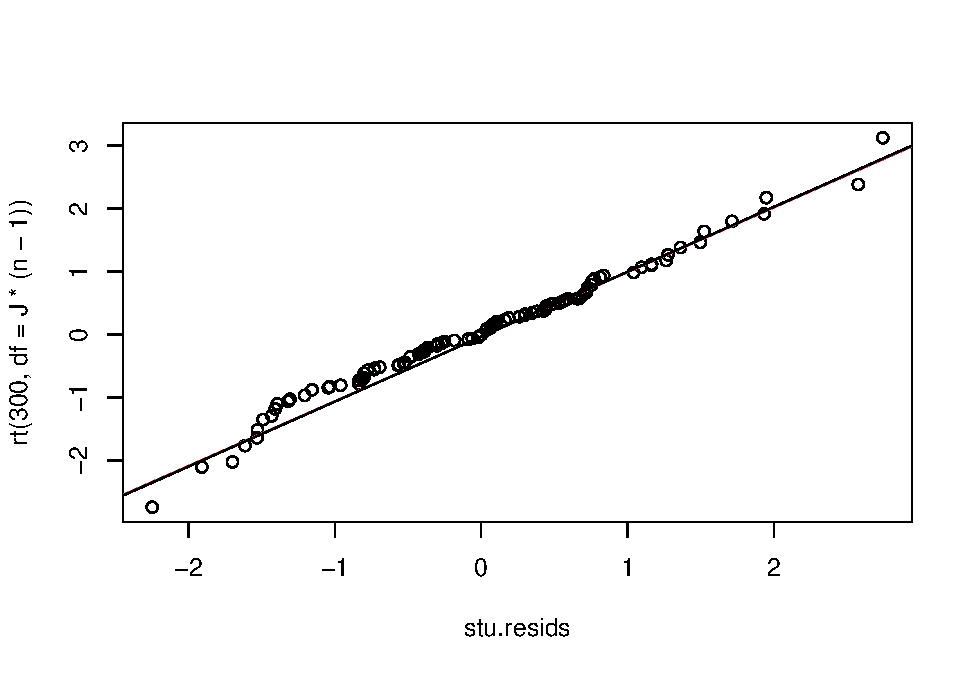
\includegraphics{14-ANOVA_files/figure-latex/unnamed-chunk-7-1.pdf}

In case the qq-plot suggests normality does NOT hold, then an alternative approximate test may be used. The Kruskal-Wallis test is similar (but not exactly the same) as performing ANOVA on the ranks \(r_{ij}\) of the responses \(y_{ij}\). Ranking means sorting the responses from least to greatest and associating each with its order in that sequence. If there are any tied values, ranks are averaged. For example, the sequence of responses \(24.3, 27.9, 27.9, 29.3, 30,1\) has ranks \(1, 2.5, 2.5, 4, 5\).

Let \(r_{ij}\) be the ranks of the \(y_{ij}\) and let \(\bar r_{i\cdot}\) and \(\bar r_{\cdot\cdot}\) be the averages of ranks in each population sample and overall, respectively. Then, the Kruskal-Wallis test statistic is the ratio of the SSB (or called SSTr) to SST of the ranks, multiplied by \(N-1\):

\[\chi^2 = (N-1) \cdot \frac{\sum_{i=1}^I n_{i}(\bar r_{i\cdot} - \bar r_{\cdot\cdot})^2}{\sum_{i=1}^I\sum_{j=1}^{n_i}(r_{ij} - \bar r_{\cdot\cdot})^2}.\]

The null hypothesis of the Kruskall-Wallis test is that the \(I\) populations are really all the same population (the \(I\) distributions are equal). In the special case in which we assume all populations are normal with the same mean, this null hypothesis is equivalent to the assertion all the means are equal. Under the Kruskal-Wallis null hypothesis, the test statistic \(\chi^2\) is \emph{approximately} distributed as a Chi-squared r.v. with \(I-1\) degrees of freedom.\\

Next, we will compute the K-W test statistic and associated p-value by hand, and then compare our results to the built-in R function ``kruskal.test''.

\begin{Shaded}
\begin{Highlighting}[]
\NormalTok{rij }\OtherTok{\textless{}{-}} \FunctionTok{rank}\NormalTok{(crops}\SpecialCharTok{$}\NormalTok{yield)}

\NormalTok{r1 }\OtherTok{\textless{}{-}} \FunctionTok{mean}\NormalTok{(rij[crops}\SpecialCharTok{$}\NormalTok{fertilizer }\SpecialCharTok{==} \DecValTok{1}\NormalTok{])}
\NormalTok{r2 }\OtherTok{\textless{}{-}} \FunctionTok{mean}\NormalTok{(rij[crops}\SpecialCharTok{$}\NormalTok{fertilizer }\SpecialCharTok{==} \DecValTok{2}\NormalTok{])}
\NormalTok{r3 }\OtherTok{\textless{}{-}} \FunctionTok{mean}\NormalTok{(rij[crops}\SpecialCharTok{$}\NormalTok{fertilizer }\SpecialCharTok{==} \DecValTok{3}\NormalTok{])}

\CommentTok{\# SSE}

\NormalTok{SSE }\OtherTok{\textless{}{-}} \FunctionTok{sum}\NormalTok{((rij[crops}\SpecialCharTok{$}\NormalTok{fertilizer }\SpecialCharTok{==} \DecValTok{1}\NormalTok{] }\SpecialCharTok{{-}}\NormalTok{ r1)}\SpecialCharTok{\^{}}\DecValTok{2}\NormalTok{)}\SpecialCharTok{+}\FunctionTok{sum}\NormalTok{((rij[crops}\SpecialCharTok{$}\NormalTok{fertilizer }\SpecialCharTok{==} \DecValTok{2}\NormalTok{] }\SpecialCharTok{{-}}\NormalTok{ r2)}\SpecialCharTok{\^{}}\DecValTok{2}\NormalTok{)}\SpecialCharTok{+}\FunctionTok{sum}\NormalTok{((rij[crops}\SpecialCharTok{$}\NormalTok{fertilizer }\SpecialCharTok{==} \DecValTok{3}\NormalTok{] }\SpecialCharTok{{-}}\NormalTok{ r3)}\SpecialCharTok{\^{}}\DecValTok{2}\NormalTok{)}
\NormalTok{SSE}
\end{Highlighting}
\end{Shaded}

\begin{verbatim}
## [1] 63603.81
\end{verbatim}

\begin{Shaded}
\begin{Highlighting}[]
\NormalTok{SST }\OtherTok{\textless{}{-}} \FunctionTok{sum}\NormalTok{((rij }\SpecialCharTok{{-}} \FunctionTok{mean}\NormalTok{(rij))}\SpecialCharTok{\^{}}\DecValTok{2}\NormalTok{)}
\NormalTok{SST}
\end{Highlighting}
\end{Shaded}

\begin{verbatim}
## [1] 73720
\end{verbatim}

\begin{Shaded}
\begin{Highlighting}[]
\CommentTok{\# SSTr}
\NormalTok{SSTr }\OtherTok{\textless{}{-}}\NormalTok{ SST}\SpecialCharTok{{-}}\NormalTok{SSE}
\NormalTok{SSTr}
\end{Highlighting}
\end{Shaded}

\begin{verbatim}
## [1] 10116.19
\end{verbatim}

\begin{Shaded}
\begin{Highlighting}[]
\NormalTok{test.stat }\OtherTok{\textless{}{-}}\NormalTok{ (n}\SpecialCharTok{*}\NormalTok{J }\SpecialCharTok{{-}} \DecValTok{1}\NormalTok{)}\SpecialCharTok{*}\NormalTok{(SSTr }\SpecialCharTok{/}\NormalTok{ SST)}
\NormalTok{test.stat}
\end{Highlighting}
\end{Shaded}

\begin{verbatim}
## [1] 13.03632
\end{verbatim}

\begin{Shaded}
\begin{Highlighting}[]
\DecValTok{1}\SpecialCharTok{{-}}\FunctionTok{pchisq}\NormalTok{(test.stat, J}\DecValTok{{-}1}\NormalTok{)}
\end{Highlighting}
\end{Shaded}

\begin{verbatim}
## [1] 0.00147638
\end{verbatim}

\begin{Shaded}
\begin{Highlighting}[]
\FunctionTok{kruskal.test}\NormalTok{(yield }\SpecialCharTok{\textasciitilde{}}\NormalTok{ fertilizer, }\AttributeTok{data =}\NormalTok{ crops)}
\end{Highlighting}
\end{Shaded}

\begin{verbatim}
## 
##  Kruskal-Wallis rank sum test
## 
## data:  yield by fertilizer
## Kruskal-Wallis chi-squared = 13.036, df = 2, p-value = 0.001476
\end{verbatim}

Note that the Kruskal-Wallis test rejects the null hypothesis that the three populations of crop yields are the same, which agrees with the ANOVA F test.

\hypertarget{simple-linear-regression}{%
\chapter{Simple Linear Regression}\label{simple-linear-regression}}

In this chapter we consider estimation and inference of a random response, conditional on another observed variable---the independent variable, also called predictor or covariate.

\hypertarget{simple-linear-regression-model}{%
\section{Simple linear regression model}\label{simple-linear-regression-model}}

The simple linear regression model says that a random response \(Y_i\) has conditional mean \(\beta_0 + \beta_1 x_i\) given \(X_i = x_i\) where \(X_i\) may be a random variable. Moreover, the responses \(Y_i\), \(i = 1, \ldots, n\), are independent, with common variance \(\sigma^2\), and are normally distributed. This is commonly written using the following statistical notation:
\[Y_i = \beta_0 + \beta_1 x_i + \epsilon_i, \quad \epsilon_i\stackrel{iid}{\sim} N(0, \sigma^2)\]
where \(\epsilon_i\) is the ``random residual''---what is left over after subtracting the mean from the response.

The model is ``linear'' because the mean \(E(Y_i|x_i) = \beta_0 + \beta_1 x_i\) is a linear function (a line in two dimensions \(y\) and \(x\)). The model is ``simple'' because it is the simplest line (two dimensions). Later we will expand the model by adding covariates, i.e., \(x_{1i}, x_{2i}, \ldots\), to the linear conditional mean function and call it \emph{multiple linear regression}.

\hypertarget{estimation}{%
\subsection{Estimation}\label{estimation}}

We estimate \((\beta_0, \beta_1)\) simultaneously using the method of ``least squares''. The method of least squares defines the line \(y = \beta_0 + \beta_1 x\) that is ``closest'' to the points \((y_i, x_i), i=1, \ldots, n\) is the one minimizing the sum of square vertical distances (residuals) from the points to the line:
\[(\hat\beta_0, \hat\beta_1) = \arg\min_{(\beta_0, \beta_1)}\sum_{i=1}^n(y_i - \beta_0 - \beta_1x_i)^2.\]
The plot below shows these residuals for three points (1.0,1.1), (1.5,2.1), and (2.0,1.8), compared to the line \(y=x\).

\begin{Shaded}
\begin{Highlighting}[]
\FunctionTok{plot}\NormalTok{(}\FunctionTok{c}\NormalTok{(}\DecValTok{1}\NormalTok{,}\FloatTok{1.5}\NormalTok{,}\DecValTok{2}\NormalTok{),}\FunctionTok{c}\NormalTok{(}\FloatTok{1.1}\NormalTok{,}\FloatTok{2.1}\NormalTok{,}\FloatTok{1.8}\NormalTok{), }\AttributeTok{xlab =} \StringTok{\textquotesingle{}x\textquotesingle{}}\NormalTok{, }\AttributeTok{ylab =} \StringTok{\textquotesingle{}y\textquotesingle{}}\NormalTok{, }\AttributeTok{main =} \StringTok{\textquotesingle{}\textquotesingle{}}\NormalTok{, }\AttributeTok{xlim =} \FunctionTok{c}\NormalTok{(}\FloatTok{0.5}\NormalTok{,}\FloatTok{2.5}\NormalTok{), }\AttributeTok{ylim =} \FunctionTok{c}\NormalTok{(}\DecValTok{0}\NormalTok{,}\DecValTok{3}\NormalTok{))}
\FunctionTok{lines}\NormalTok{(}\FunctionTok{c}\NormalTok{(}\FloatTok{0.5}\NormalTok{,}\FloatTok{2.5}\NormalTok{),}\FunctionTok{c}\NormalTok{(}\FloatTok{0.5}\NormalTok{,}\FloatTok{2.5}\NormalTok{))}
\FunctionTok{lines}\NormalTok{(}\FunctionTok{c}\NormalTok{(}\DecValTok{1}\NormalTok{,}\DecValTok{1}\NormalTok{), }\FunctionTok{c}\NormalTok{(}\DecValTok{1}\NormalTok{,}\FloatTok{1.1}\NormalTok{), }\AttributeTok{lty =} \DecValTok{3}\NormalTok{)}
\FunctionTok{lines}\NormalTok{(}\FunctionTok{c}\NormalTok{(}\FloatTok{1.5}\NormalTok{,}\FloatTok{1.5}\NormalTok{), }\FunctionTok{c}\NormalTok{(}\FloatTok{1.5}\NormalTok{,}\FloatTok{2.1}\NormalTok{), }\AttributeTok{lty =} \DecValTok{3}\NormalTok{)}
\FunctionTok{lines}\NormalTok{(}\FunctionTok{c}\NormalTok{(}\DecValTok{2}\NormalTok{,}\DecValTok{2}\NormalTok{), }\FunctionTok{c}\NormalTok{(}\DecValTok{2}\NormalTok{,}\FloatTok{1.8}\NormalTok{), }\AttributeTok{lty =} \DecValTok{3}\NormalTok{)}
\end{Highlighting}
\end{Shaded}

\includegraphics{15-Regression_files/figure-latex/unnamed-chunk-1-1.pdf}

We can determine the estimators \((\hat\beta_0, \hat\beta_1)\) by minimizing the sum of squared residuals using calculus:

\[
\begin{aligned}
\frac{\partial}{\partial\beta_0} \sum_{i=1}^n(y_i - \beta_0 - \beta_1x_i)^2 \\
& = -2\sum_{i=1}^n(y_i - \beta_0 - \beta_1x_i)\\
\text{set  }0 &= -2\sum_{i=1}^n(y_i - \beta_0 - \beta_1x_i)\\
&\Rightarrow \hat\beta_0 = n^{-1}\sum_{i=1}^n(y_i - \beta_1x_i)\\
& = \bar y - \beta_1\bar x
\end{aligned}
\]

\[
\begin{aligned}
\frac{\partial}{\partial\beta_1} \sum_{i=1}^n(y_i - \beta_0 - \beta_1x_i)^2 \\
& = -2 \sum_{i=1}^n x_i(y_i - \beta_0 - \beta_1x_i)\\
\text{set  }0 &= -2 \sum_{i=1}^n x_i(y_i - \beta_0 - \beta_1x_i)\\
&\Rightarrow 0 = \sum_{i=1}^n (y_ix_i - x_i(\bar y - \beta_1 \bar x) - \beta_1 x_i^2)\quad \text{by substituting }\beta_0\\
& \beta_1\sum(x_i^2 - x_i\bar x) = \sum_{i=1}^n(y_ix_i - \bar y x_i)\\
&\Rightarrow \hat\beta_1 = \frac{\sum_{i=1}^n (y_ix_i) - n\bar y\bar x}{\sum_{i=1}^n 
(x_i^2) - n\bar x^2} = \frac{\sum_{i=1}^n [(y_i - \bar y)(x_i - \bar x)]}{\sum_{i=1}^n (x_i - \bar x)^2}
\end{aligned}
\]
\#\#\# LSEs are unbiased

A nice property of the least squares method is that it produces unbiased estimators. Consider the expectation \(E(\hat\beta_1)\). Since the \(x_i'\)s are non-random, treat these as constants, and find \(\hat\beta_1\) is unbiased:

\[
\begin{aligned}
E(\hat\beta_1) & = \frac{\sum_{i=1}^n E((y_i - \bar y))(x_i - \bar x)}{\sum_{i=1}^n (x_i - \bar x)^2}\\
& = \frac{\sum_{i=1}^n (\beta_0 + \beta_1 x_i - n^{-1}\sum_{i=1}^n [\beta_0 +\beta_1 x_i])(x_i - \bar x)}{\sum_{i=1}^n (x_i - \bar x)^2}\\
& = \frac{\beta_1\sum_{i=1}^n ( x_i - \bar x)(x_i - \bar x)}{\sum_{i=1}^n (x_i - \bar x)^2}\\
& = \beta_1.
\end{aligned}
\]

Similarly, the estimator of the intercept is unbiased:

\[
\begin{aligned}
E(\hat\beta_0) & = E(\bar y - \hat\beta_1 \bar x)\\
& = n^{-1}\sum_{i=1}^n (\beta_0 + \beta_1x_i) - \beta_1 \bar x\\
& = \beta_0 + \beta_1 \bar x - \beta_1 \bar x\\
& = \beta_0
\end{aligned}
\]

\hypertarget{estimation-of-the-common-variance}{%
\subsection{Estimation of the common variance}\label{estimation-of-the-common-variance}}

Estimating \(\sigma^2\) in the regression model is similar to the method used in ANOVA. Define the observed/fitted residuals \(\hat e_i = y_i - \hat y_i = y_i - \hat\beta_0 - \hat\beta_1 x_i\). Since \((\hat\beta_0, \hat\beta_1)\) are unbiased, we have \(E(\hat e_i) = E(Y_i - \hat\beta_0 - \hat\beta_1 x_i) = 0\). Therefore, \(V(\hat e_i) = E(\hat e_i ^2)\). And, the method of moments suggests we estimate the variance(in this case second moment) by the sample variance:

\[\hat\sigma^2 = \frac{1}{n-2}\sum_{i=1}^n (y_i - \hat\beta_0 - \hat\beta_1 x_i)^2,\]
where we divide by \(n-2\) so that the resulting estimator is unbiased. (I'll leave that as a challenging exercise for the reader).

\hypertarget{inference-for-regression-slope-parameter}{%
\subsection{Inference for regression slope parameter}\label{inference-for-regression-slope-parameter}}

There are two main inference (and prediction) problems of interest in regression. The first is inference on \(\beta_1\), and, in particular, testing \(\beta_1 = 0\). If \(\beta_1=0\) then there is no linear relationship between the covariate \(x\) and the response \(Y\), and \(Y\) has a constant mean (so is iid, rather than independent). Testing \(\beta_1=0\) is similar to the ANOVA F test for categorical \(x\), rather than continuous \(x\) in regression.\\

For inference on \(\beta_1\) we need the sampling distribution of \(\hat\beta_1\). Recognize that we can write this estimator as
\[\hat\beta_1 = \frac{\sum_{i=1}^n Y_i(x_i - \bar x)}{\sum_{i=1}^n (x_i - \bar x)^2}\] because \(\sum_{i=1}^n \bar Y(x_i - \bar x) = 0\). Then, we see that \(\hat\beta_1\) is a linear combination of \(Y_i\), i.e., \(\hat\beta_1 = \sum_{i=1}^nc_i Y_i\) for non-random \(c_i\). By a MGF argument we have used before, linear combinations of normal random variables are also normally-distributed. This means,
\[\hat\beta_1 \sim N\left(\beta_1, \sigma_2\sum_{i=1}^n c_i^2\right).\]

Furthermore, by essentially the same argument as in the proof of Student's Theorem,
\[\frac{(n-2)\hat\sigma^2}{\sigma^2}\sim \chi^2(n-2)\]
so that the studentized slope estimator has a Student's \(t\) distribution:
\[t = \frac{\hat\beta_1 - \beta_1}{\sqrt{\hat\sigma^2 \left[\sum_{i=1}^n (x_i - \bar x)^2\right]^{-1}}}\sim t_{n-2}\]

A test of \(H_0:\beta_1 = b\) versus \(H_a:\beta_1 \ne b\) rejects the null if
\[\frac{|\hat\beta_1 - b|}{\sqrt{\hat\sigma^2 \left[\sum_{i=1}^n (x_i - \bar x)^2\right]^{-1}}} > t_{1-\alpha/2, n-2}\]

Similarly, a \(100(1-\alpha)\%\) CI for \(\beta_1\) is given by
\[\left(\hat\beta_1 \pm t_{1-\alpha/2, n-2}\sqrt{\hat\sigma^2 \left[\sum_{i=1}^n (x_i - \bar x)^2\right]^{-1}}\right).\]

\hypertarget{inference-on-the-conditional-mean-response}{%
\subsection{Inference on the conditional mean response}\label{inference-on-the-conditional-mean-response}}

Besides testing for \(H_0:\beta_1 = 0\), which means that the covariate has no effect on the mean response, experimenters often want to make inferences about the conditional mean response at a particular covariate value \(x\). As we showed above, \(\hat\beta_0 + \hat\beta_1 x\) is unbiased for \(E(Y|x) = \beta_0 + \beta_1 x\). Furthermore, the variance of the estimator of the conditional mean is as follows:

\begin{align*}
V(\hat\beta_0 + \hat\beta_1 x) &= V(\overline Y - \hat\beta_1 \overline x + \hat\beta_1 x) \\
& = V\left(\overline Y + (x - \overline x)\frac{\sum Y_i(x_i - \overline x)}{\sum (x_i - \overline x)^2}\right)\\
& = V\left( \sum Y_i \left(n^{-1} + (x - \overline x)\frac{(x_i - \overline x)}{\sum (x_i - \overline x)^2}\right)\right)\\
& = \sum_{i=1}^n V\left(Y_i\left(n^{-1} + (x - \overline x)\frac{(x_i - \overline x)}{\sum (x_i - \overline x)^2}\right)\right)\\
& = \sigma^2\sum_{i=1}^n \frac{1}{n^2} + \frac{(x - \overline x)^2(x_i - \overline x)^2}{\left[\sum (x_i - \overline x)^2\right]^2}\\
& = \sigma^2\left(n^{-1} + \frac{(x - \overline x)^2}{\sum (x_i - \overline x)^2}\right)
\end{align*}

Replacing the unknown variance \(\sigma^2\) by its estimator (the MSE) we obtain a Student's \(t\) random variable with \(n-2\) degrees of freedom:
\[t = \frac{\hat\beta_0 + \hat\beta_1 x  - (\beta_0 + \beta_1 x)}{\sqrt{MSE \left(n^{-1} + \frac{(x - \overline x)^2}{\sum (x_i - \overline x)^2}\right)}}\sim t_{n-2}.\]

This may be used to define a confidence interval for the conditional mean response at a given covariate value \(x\):

\[\left(\hat\beta_0 + \hat\beta_1 x \pm t_{1-\alpha/2, n-2}\sqrt{MSE \left(n^{-1} + \frac{(x - \overline x)^2}{\sum (x_i - \overline x)^2}\right)}  \right)\]

\hypertarget{prediction-of-responses-at-given-x-values}{%
\subsection{Prediction of responses at given x values}\label{prediction-of-responses-at-given-x-values}}

Let \(Y^\star\) denote a future response for a given covariate value \(x\). We want to predict \(Y^\star\sim N(\beta_0 + \beta_1 x, \sigma^2)\). Now, we can represent \(Y^\star\) using the regression model as
\[Y^\star = \beta_0 + \beta_1 x + \epsilon^\star\]
for a future random residual \(\epsilon^\star\). An unbiased point prediction of \(Y^\star\) is given by the estimate of its mean \(\hat\beta_0 + \hat\beta_1 x\). The variance of the point prediction is
\[V(\hat{Y^\star}) = V(\hat\beta_0 + \hat\beta_1 x + \epsilon^\star) = \sigma^2\left(1 +n^{-1} + \frac{(x - \overline x)^2}{\sum (x_i - \overline x)^2}\right).\]

Therefore, a \(100(1-\alpha)\%\) prediction interval for \(Y^\star\) is given by
\[\left(\hat\beta_0 + \hat\beta_1 x \pm t_{1-\alpha/2, n-2}\sqrt{MSE \left(1 +n^{-1} + \frac{(x - \overline x)^2}{\sum (x_i - \overline x)^2}\right)}  \right).\]

Prediction intervals have interpretations similar to confidence intervals. If the model is true, a \(95\%\) prediction interval for \(Y^\star\) at a given \(x\) has the following property: suppose we repeat a regression experiment many, many times. Each time we compute a \(95\%\) interval and then observe a new response \(Y^\star\). then, about \(95\%\) of the time, our computed prediction interval contains that realized \(Y^\star\). This is easiest to see given a simulation experiment.

\begin{Shaded}
\begin{Highlighting}[]
\NormalTok{x }\OtherTok{\textless{}{-}} \DecValTok{1}\SpecialCharTok{:}\DecValTok{10}  \CommentTok{\# covariate values are 1, 2, 3, 4, 5, 6, 7, 8, 9, 10}
\NormalTok{cover }\OtherTok{\textless{}{-}} \FunctionTok{rep}\NormalTok{(}\DecValTok{0}\NormalTok{,}\DecValTok{1000}\NormalTok{) }\CommentTok{\# record whether the prediction interval contains the new response Y*}
\ControlFlowTok{for}\NormalTok{(r }\ControlFlowTok{in} \DecValTok{1}\SpecialCharTok{:}\DecValTok{1000}\NormalTok{)\{  }\CommentTok{\# loop 1000 "experiments"}
\NormalTok{Y }\OtherTok{\textless{}{-}} \FunctionTok{rnorm}\NormalTok{(}\DecValTok{10}\NormalTok{,}\DecValTok{1}\SpecialCharTok{+}\DecValTok{2}\SpecialCharTok{*}\NormalTok{x)  }\CommentTok{\# randomly sample the responses }
\NormalTok{my.lm }\OtherTok{\textless{}{-}} \FunctionTok{summary}\NormalTok{(}\FunctionTok{lm}\NormalTok{(Y}\SpecialCharTok{\textasciitilde{}}\NormalTok{x))  }\CommentTok{\# compute the point estimates of beta0, beta1 and sigma\^{}2}
\NormalTok{MSE }\OtherTok{\textless{}{-}} \FunctionTok{sum}\NormalTok{(my.lm}\SpecialCharTok{$}\NormalTok{residuals}\SpecialCharTok{\^{}}\DecValTok{2}\NormalTok{)}\SpecialCharTok{/}\DecValTok{8} \CommentTok{\# point estimate of sigma\^{}2}
\NormalTok{beta0.hat }\OtherTok{\textless{}{-}}\NormalTok{ my.lm}\SpecialCharTok{$}\NormalTok{coefficients[}\DecValTok{1}\NormalTok{] }\CommentTok{\# storing the estimates of beta0 and beta 1}
\NormalTok{beta1.hat }\OtherTok{\textless{}{-}}\NormalTok{ my.lm}\SpecialCharTok{$}\NormalTok{coefficients[}\DecValTok{2}\NormalTok{]}
\NormalTok{mean.hat }\OtherTok{\textless{}{-}}\NormalTok{ beta0.hat }\SpecialCharTok{+}\NormalTok{ beta1.hat}\SpecialCharTok{*}\DecValTok{4} \CommentTok{\# the estimated conditional mean response}
\NormalTok{se.term }\OtherTok{\textless{}{-}}\NormalTok{ (}\DecValTok{1}\SpecialCharTok{+}\DecValTok{1}\SpecialCharTok{/}\DecValTok{10} \SpecialCharTok{+}\NormalTok{ ((}\DecValTok{4}\SpecialCharTok{{-}}\FunctionTok{mean}\NormalTok{(x))}\SpecialCharTok{\^{}}\DecValTok{2}\NormalTok{) }\SpecialCharTok{/}\NormalTok{ (}\FunctionTok{sum}\NormalTok{((x}\SpecialCharTok{{-}}\FunctionTok{mean}\NormalTok{(x))}\SpecialCharTok{\^{}}\DecValTok{2}\NormalTok{))) }\CommentTok{\# the 1 + 1/n + (x{-}xbar)\^{}2/sum(xi {-} xbar)\^{}2 term in the standard error}
\NormalTok{my.PI }\OtherTok{\textless{}{-}} \FunctionTok{c}\NormalTok{(mean.hat }\SpecialCharTok{+} \FunctionTok{qt}\NormalTok{(}\FloatTok{0.025}\NormalTok{,}\DecValTok{8}\NormalTok{)}\SpecialCharTok{*}\FunctionTok{sqrt}\NormalTok{(MSE}\SpecialCharTok{*}\NormalTok{se.term), mean.hat }\SpecialCharTok{+} \FunctionTok{qt}\NormalTok{(}\FloatTok{0.975}\NormalTok{,}\DecValTok{8}\NormalTok{)}\SpecialCharTok{*}\FunctionTok{sqrt}\NormalTok{(MSE}\SpecialCharTok{*}\NormalTok{se.term)) }\CommentTok{\# prediction intervals}
\NormalTok{Y.star }\OtherTok{\textless{}{-}} \FunctionTok{rnorm}\NormalTok{(}\DecValTok{1}\NormalTok{,}\DecValTok{1}\SpecialCharTok{+}\DecValTok{2}\SpecialCharTok{*}\DecValTok{4}\NormalTok{) }\CommentTok{\# sample a new response Y*}
\NormalTok{cover[r] }\OtherTok{\textless{}{-}} \FunctionTok{ifelse}\NormalTok{(my.PI[}\DecValTok{1}\NormalTok{] }\SpecialCharTok{\textless{}}\NormalTok{ Y.star }\SpecialCharTok{\&}\NormalTok{ my.PI[}\DecValTok{2}\NormalTok{] }\SpecialCharTok{\textgreater{}}\NormalTok{ Y.star, }\DecValTok{1}\NormalTok{, }\DecValTok{0}\NormalTok{) }\CommentTok{\# check if interval contains ("covers") the Y*}
\NormalTok{\}}
\FunctionTok{mean}\NormalTok{(cover)  }\CommentTok{\# realized coverage proportion, should be about 95\%}
\end{Highlighting}
\end{Shaded}

\begin{verbatim}
## [1] 0.959
\end{verbatim}

\hypertarget{simultaneous-confidence-bands-for-the-regression-line}{%
\subsection{Simultaneous confidence bands for the regression line}\label{simultaneous-confidence-bands-for-the-regression-line}}

If experimenters want to quantify uncertainty about the entire regression line, then we may compute simultaneous confidence bands. The interpretation of these bands is similar to the interpretation of a confidence interval for a ream response at a given \(x\), except the object we are claiming to capture by the bands is the line itself, rather than a point on the line.

We may construct such bands based on simultaneous confidence intervals for the two parameters the line depends on, which are \((\beta_0, \beta_1)\). By \emph{simultaneous}, we mean a confidence set (in two dimensions) that has probability \(100(1-\alpha)\%\) to capture the point \((\beta_0, \beta_1)\) with respect to repeated experimentation/random sampling.

The Scheffe method may be used to construct simultaneous CIs for \((\beta_0, \beta_1)\). The Scheffe simultaneous CIs are given by
\[\left(\hat\beta_0 \pm \sqrt{\frac{2F_{1-\alpha, 2, n-2}MSE n^{-1}\sum x_i^2}{\sum(x_i - \overline x)^2}}\right),\]
and
\[\left(\hat\beta_1 \pm \sqrt{\frac{2F_{1-\alpha, 2, n-2}MSE }{\sum(x_i - \overline x)^2}}\right).\]

A simultaneous confidence band for \(\beta_0 + \beta_1 x\) over \(x \in (a,b)\) has lower bound \(b_0 + b_1 x\) and upper bound \(B_0 +B_1 x\) where \(b_0\) and \(b_1\) are the lower bounds of the simultaneous CIs of \(\beta_0\) and \(\beta_1\) and \(B_0\) and \(B_1\) are the upper bounds.

\hypertarget{example-house-prices-as-function-of-house-age}{%
\section{Example: House prices as function of house age}\label{example-house-prices-as-function-of-house-age}}

\begin{Shaded}
\begin{Highlighting}[]
\NormalTok{houses }\OtherTok{\textless{}{-}} \FunctionTok{read.csv}\NormalTok{(}\StringTok{"Real estate.csv"}\NormalTok{, }\AttributeTok{header =} \ConstantTok{TRUE}\NormalTok{)}
\FunctionTok{plot}\NormalTok{(houses}\SpecialCharTok{$}\NormalTok{X2.house.age, houses}\SpecialCharTok{$}\NormalTok{Y.house.price.of.unit.area, }\AttributeTok{xlab =} \StringTok{\textquotesingle{}age\textquotesingle{}}\NormalTok{, }\AttributeTok{ylab =} \StringTok{\textquotesingle{}price by unit area\textquotesingle{}}\NormalTok{)}
\end{Highlighting}
\end{Shaded}

\includegraphics{15-Regression_files/figure-latex/unnamed-chunk-4-1.pdf}

\hypertarget{fitting-the-regression}{%
\subsection{Fitting the regression}\label{fitting-the-regression}}

From the output of the summary of teh lm fit we see that the fitted regression line is
\[\text{Price by unit area } = 42.4347 - 0.2515\text{ age}. \]
The estimated variance is \(MSE = \hat\sigma^2 = 13.32^2\).

We have the observed test statistics:
\[\frac{\hat\beta_0}{\sqrt{\frac{MSE n^{-1}\sum x_i^2}{\sum(x_i - \overline x)^2}}} = 35.042\]
and
\[\frac{\hat\beta_1}{\sqrt{\frac{MSE }{\sum(x_i - \overline x)^2}}} = -4.372\]
which are both significant, meaning the intercept and slope are not zero.

\begin{Shaded}
\begin{Highlighting}[]
\NormalTok{my.lm }\OtherTok{\textless{}{-}} \FunctionTok{lm}\NormalTok{(Y.house.price.of.unit.area}\SpecialCharTok{\textasciitilde{}}\NormalTok{X2.house.age, }\AttributeTok{data =}\NormalTok{ houses)}
\FunctionTok{summary}\NormalTok{(my.lm)}
\end{Highlighting}
\end{Shaded}

\begin{verbatim}
## 
## Call:
## lm(formula = Y.house.price.of.unit.area ~ X2.house.age, data = houses)
## 
## Residuals:
##     Min      1Q  Median      3Q     Max 
## -31.113 -10.738   1.626   8.199  77.781 
## 
## Coefficients:
##              Estimate Std. Error t value Pr(>|t|)    
## (Intercept)  42.43470    1.21098  35.042  < 2e-16 ***
## X2.house.age -0.25149    0.05752  -4.372 1.56e-05 ***
## ---
## Signif. codes:  0 '***' 0.001 '**' 0.01 '*' 0.05 '.' 0.1 ' ' 1
## 
## Residual standard error: 13.32 on 412 degrees of freedom
## Multiple R-squared:  0.04434,    Adjusted R-squared:  0.04202 
## F-statistic: 19.11 on 1 and 412 DF,  p-value: 1.56e-05
\end{verbatim}

The fitted line, overlaid on the data:

\begin{Shaded}
\begin{Highlighting}[]
\NormalTok{houses }\OtherTok{\textless{}{-}} \FunctionTok{read.csv}\NormalTok{(}\StringTok{"Real estate.csv"}\NormalTok{, }\AttributeTok{header =} \ConstantTok{TRUE}\NormalTok{)}
\FunctionTok{plot}\NormalTok{(houses}\SpecialCharTok{$}\NormalTok{X2.house.age, houses}\SpecialCharTok{$}\NormalTok{Y.house.price.of.unit.area, }\AttributeTok{xlab =} \StringTok{\textquotesingle{}age\textquotesingle{}}\NormalTok{, }\AttributeTok{ylab =} \StringTok{\textquotesingle{}price by unit area\textquotesingle{}}\NormalTok{)}
\FunctionTok{abline}\NormalTok{(}\AttributeTok{a =} \FloatTok{42.43470}\NormalTok{, }\AttributeTok{b =} \SpecialCharTok{{-}}\NormalTok{.}\DecValTok{25149}\NormalTok{, }\AttributeTok{col =} \StringTok{\textquotesingle{}blue\textquotesingle{}}\NormalTok{, }\AttributeTok{lwd =} \DecValTok{2}\NormalTok{)}
\end{Highlighting}
\end{Shaded}

\includegraphics{15-Regression_files/figure-latex/unnamed-chunk-6-1.pdf}

Predicting the home price of a house that is 20 years old:

\begin{Shaded}
\begin{Highlighting}[]
\NormalTok{my.summ }\OtherTok{\textless{}{-}} \FunctionTok{summary}\NormalTok{(my.lm)}
\NormalTok{MSE }\OtherTok{\textless{}{-}}\NormalTok{ my.summ}\SpecialCharTok{$}\NormalTok{sigma}\SpecialCharTok{\^{}}\DecValTok{2}
\NormalTok{n}\OtherTok{\textless{}{-}} \FunctionTok{length}\NormalTok{(houses}\SpecialCharTok{$}\NormalTok{Y.house.price.of.unit.area)}
\NormalTok{se.term }\OtherTok{\textless{}{-}} \DecValTok{1}\SpecialCharTok{+} \DecValTok{1}\SpecialCharTok{/}\NormalTok{n }\SpecialCharTok{+}\NormalTok{ ((}\DecValTok{20}\SpecialCharTok{{-}}\FunctionTok{mean}\NormalTok{(houses}\SpecialCharTok{$}\NormalTok{X2.house.age))}\SpecialCharTok{\^{}}\DecValTok{2}\NormalTok{) }\SpecialCharTok{/} \FunctionTok{sum}\NormalTok{((houses}\SpecialCharTok{$}\NormalTok{X2.house.age }\SpecialCharTok{{-}} \FunctionTok{mean}\NormalTok{(houses}\SpecialCharTok{$}\NormalTok{X2.house.age))}\SpecialCharTok{\^{}}\DecValTok{2}\NormalTok{)}
\NormalTok{PI }\OtherTok{\textless{}{-}} \FunctionTok{c}\NormalTok{(my.summ}\SpecialCharTok{$}\NormalTok{coefficients[}\DecValTok{1}\NormalTok{] }\SpecialCharTok{+}\NormalTok{ my.summ}\SpecialCharTok{$}\NormalTok{coefficients[}\DecValTok{2}\NormalTok{]}\SpecialCharTok{*}\DecValTok{20} \SpecialCharTok{+} \FunctionTok{qt}\NormalTok{(}\FloatTok{0.025}\NormalTok{, my.summ}\SpecialCharTok{$}\NormalTok{df[}\DecValTok{2}\NormalTok{])}\SpecialCharTok{*}\FunctionTok{sqrt}\NormalTok{(MSE}\SpecialCharTok{*}\NormalTok{se.term), my.summ}\SpecialCharTok{$}\NormalTok{coefficients[}\DecValTok{1}\NormalTok{] }\SpecialCharTok{+}\NormalTok{ my.summ}\SpecialCharTok{$}\NormalTok{coefficients[}\DecValTok{2}\NormalTok{]}\SpecialCharTok{*}\DecValTok{20} \SpecialCharTok{+} \FunctionTok{qt}\NormalTok{(}\FloatTok{0.975}\NormalTok{, my.summ}\SpecialCharTok{$}\NormalTok{df[}\DecValTok{2}\NormalTok{])}\SpecialCharTok{*}\FunctionTok{sqrt}\NormalTok{(MSE}\SpecialCharTok{*}\NormalTok{se.term))}
\NormalTok{PI}
\end{Highlighting}
\end{Shaded}

\begin{verbatim}
## [1] 11.19322 63.61663
\end{verbatim}

\begin{Shaded}
\begin{Highlighting}[]
\NormalTok{houses }\OtherTok{\textless{}{-}} \FunctionTok{read.csv}\NormalTok{(}\StringTok{"Real estate.csv"}\NormalTok{, }\AttributeTok{header =} \ConstantTok{TRUE}\NormalTok{)}
\FunctionTok{plot}\NormalTok{(houses}\SpecialCharTok{$}\NormalTok{X2.house.age, houses}\SpecialCharTok{$}\NormalTok{Y.house.price.of.unit.area, }\AttributeTok{xlab =} \StringTok{\textquotesingle{}age\textquotesingle{}}\NormalTok{, }\AttributeTok{ylab =} \StringTok{\textquotesingle{}price by unit area\textquotesingle{}}\NormalTok{)}
\FunctionTok{abline}\NormalTok{(}\AttributeTok{a =} \FloatTok{42.43470}\NormalTok{, }\AttributeTok{b =} \SpecialCharTok{{-}}\NormalTok{.}\DecValTok{25149}\NormalTok{, }\AttributeTok{col =} \StringTok{\textquotesingle{}blue\textquotesingle{}}\NormalTok{, }\AttributeTok{lwd =} \DecValTok{2}\NormalTok{)}
\FunctionTok{lines}\NormalTok{(}\FunctionTok{c}\NormalTok{(}\DecValTok{20}\NormalTok{,}\DecValTok{20}\NormalTok{), PI, }\AttributeTok{col =} \StringTok{\textquotesingle{}red\textquotesingle{}}\NormalTok{, }\AttributeTok{type =} \StringTok{\textquotesingle{}o\textquotesingle{}}\NormalTok{)}
\end{Highlighting}
\end{Shaded}

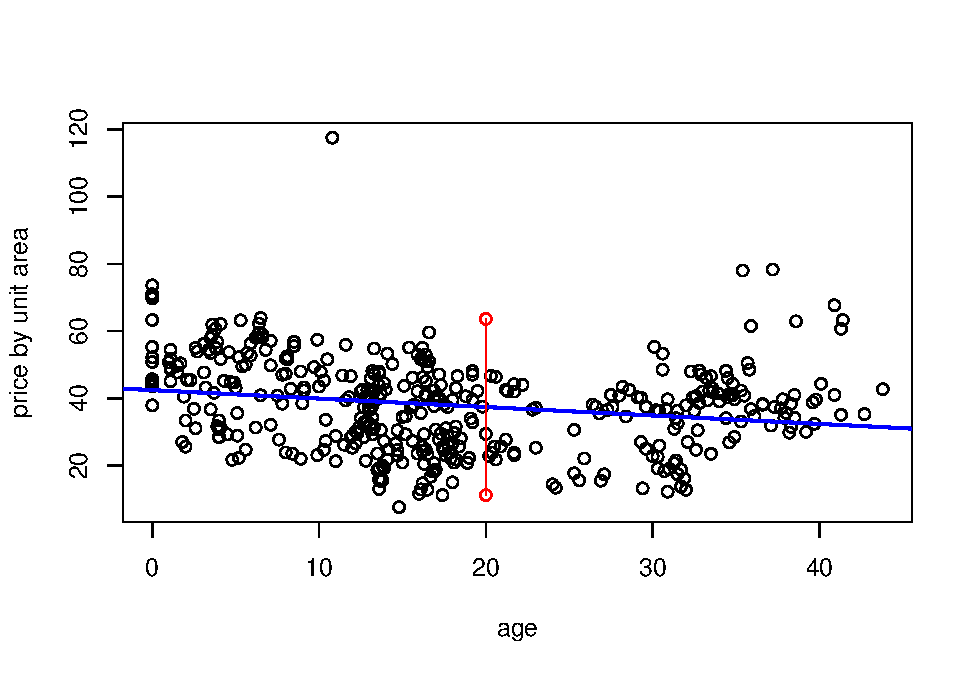
\includegraphics{15-Regression_files/figure-latex/unnamed-chunk-8-1.pdf}

Simultaneous Confidence bands:

\begin{Shaded}
\begin{Highlighting}[]
\NormalTok{my.summ }\OtherTok{\textless{}{-}} \FunctionTok{summary}\NormalTok{(my.lm)}
\NormalTok{MSE }\OtherTok{\textless{}{-}}\NormalTok{ my.summ}\SpecialCharTok{$}\NormalTok{sigma}\SpecialCharTok{\^{}}\DecValTok{2}
\NormalTok{n}\OtherTok{\textless{}{-}} \FunctionTok{length}\NormalTok{(houses}\SpecialCharTok{$}\NormalTok{Y.house.price.of.unit.area)}
\NormalTok{se.term0 }\OtherTok{\textless{}{-}}\NormalTok{ (}\DecValTok{1}\SpecialCharTok{/}\NormalTok{n)}\SpecialCharTok{*}\FunctionTok{sum}\NormalTok{(houses}\SpecialCharTok{$}\NormalTok{X2.house.age}\SpecialCharTok{\^{}}\DecValTok{2}\NormalTok{)}\SpecialCharTok{/}\FunctionTok{sum}\NormalTok{((houses}\SpecialCharTok{$}\NormalTok{X2.house.age }\SpecialCharTok{{-}} \FunctionTok{mean}\NormalTok{(houses}\SpecialCharTok{$}\NormalTok{X2.house.age))}\SpecialCharTok{\^{}}\DecValTok{2}\NormalTok{)}
\NormalTok{se.term1 }\OtherTok{\textless{}{-}} \DecValTok{1}\SpecialCharTok{/}\FunctionTok{sum}\NormalTok{((houses}\SpecialCharTok{$}\NormalTok{X2.house.age }\SpecialCharTok{{-}} \FunctionTok{mean}\NormalTok{(houses}\SpecialCharTok{$}\NormalTok{X2.house.age))}\SpecialCharTok{\^{}}\DecValTok{2}\NormalTok{)}

\NormalTok{beta0.intv }\OtherTok{\textless{}{-}} \FunctionTok{c}\NormalTok{(my.summ}\SpecialCharTok{$}\NormalTok{coefficients[}\DecValTok{1}\NormalTok{] }\SpecialCharTok{{-}} \FunctionTok{sqrt}\NormalTok{(}\DecValTok{2}\SpecialCharTok{*}\FunctionTok{qf}\NormalTok{(}\FloatTok{0.95}\NormalTok{,}\DecValTok{2}\NormalTok{,my.summ}\SpecialCharTok{$}\NormalTok{df[}\DecValTok{2}\NormalTok{])}\SpecialCharTok{*}\NormalTok{MSE}\SpecialCharTok{*}\NormalTok{se.term0), my.summ}\SpecialCharTok{$}\NormalTok{coefficients[}\DecValTok{1}\NormalTok{] }\SpecialCharTok{+} \FunctionTok{sqrt}\NormalTok{(}\DecValTok{2}\SpecialCharTok{*}\FunctionTok{qf}\NormalTok{(}\FloatTok{0.95}\NormalTok{,}\DecValTok{2}\NormalTok{,my.summ}\SpecialCharTok{$}\NormalTok{df[}\DecValTok{2}\NormalTok{])}\SpecialCharTok{*}\NormalTok{MSE}\SpecialCharTok{*}\NormalTok{se.term0))}
\NormalTok{beta1.intv }\OtherTok{\textless{}{-}} \FunctionTok{c}\NormalTok{(my.summ}\SpecialCharTok{$}\NormalTok{coefficients[}\DecValTok{2}\NormalTok{] }\SpecialCharTok{{-}} \FunctionTok{sqrt}\NormalTok{(}\DecValTok{2}\SpecialCharTok{*}\FunctionTok{qf}\NormalTok{(}\FloatTok{0.95}\NormalTok{,}\DecValTok{2}\NormalTok{,my.summ}\SpecialCharTok{$}\NormalTok{df[}\DecValTok{2}\NormalTok{])}\SpecialCharTok{*}\NormalTok{MSE}\SpecialCharTok{*}\NormalTok{se.term1), my.summ}\SpecialCharTok{$}\NormalTok{coefficients[}\DecValTok{2}\NormalTok{] }\SpecialCharTok{+} \FunctionTok{sqrt}\NormalTok{(}\DecValTok{2}\SpecialCharTok{*}\FunctionTok{qf}\NormalTok{(}\FloatTok{0.95}\NormalTok{,}\DecValTok{2}\NormalTok{,my.summ}\SpecialCharTok{$}\NormalTok{df[}\DecValTok{2}\NormalTok{])}\SpecialCharTok{*}\NormalTok{MSE}\SpecialCharTok{*}\NormalTok{se.term1))}
\end{Highlighting}
\end{Shaded}

\begin{Shaded}
\begin{Highlighting}[]
\NormalTok{houses }\OtherTok{\textless{}{-}} \FunctionTok{read.csv}\NormalTok{(}\StringTok{"Real estate.csv"}\NormalTok{, }\AttributeTok{header =} \ConstantTok{TRUE}\NormalTok{)}
\FunctionTok{plot}\NormalTok{(houses}\SpecialCharTok{$}\NormalTok{X2.house.age, houses}\SpecialCharTok{$}\NormalTok{Y.house.price.of.unit.area, }\AttributeTok{xlab =} \StringTok{\textquotesingle{}age\textquotesingle{}}\NormalTok{, }\AttributeTok{ylab =} \StringTok{\textquotesingle{}price by unit area\textquotesingle{}}\NormalTok{)}
\FunctionTok{abline}\NormalTok{(}\AttributeTok{a =} \FloatTok{42.43470}\NormalTok{, }\AttributeTok{b =} \SpecialCharTok{{-}}\NormalTok{.}\DecValTok{25149}\NormalTok{, }\AttributeTok{col =} \StringTok{\textquotesingle{}blue\textquotesingle{}}\NormalTok{, }\AttributeTok{lwd =} \DecValTok{2}\NormalTok{)}
\FunctionTok{abline}\NormalTok{(}\AttributeTok{a =}\NormalTok{ beta0.intv[}\DecValTok{1}\NormalTok{], }\AttributeTok{b =}\NormalTok{ beta1.intv[}\DecValTok{1}\NormalTok{], }\AttributeTok{col =} \StringTok{\textquotesingle{}red\textquotesingle{}}\NormalTok{, }\AttributeTok{lwd =} \DecValTok{2}\NormalTok{)}
\FunctionTok{abline}\NormalTok{(}\AttributeTok{a =}\NormalTok{ beta0.intv[}\DecValTok{2}\NormalTok{], }\AttributeTok{b =}\NormalTok{ beta1.intv[}\DecValTok{2}\NormalTok{], }\AttributeTok{col =} \StringTok{\textquotesingle{}red\textquotesingle{}}\NormalTok{, }\AttributeTok{lwd =} \DecValTok{2}\NormalTok{)}
\end{Highlighting}
\end{Shaded}

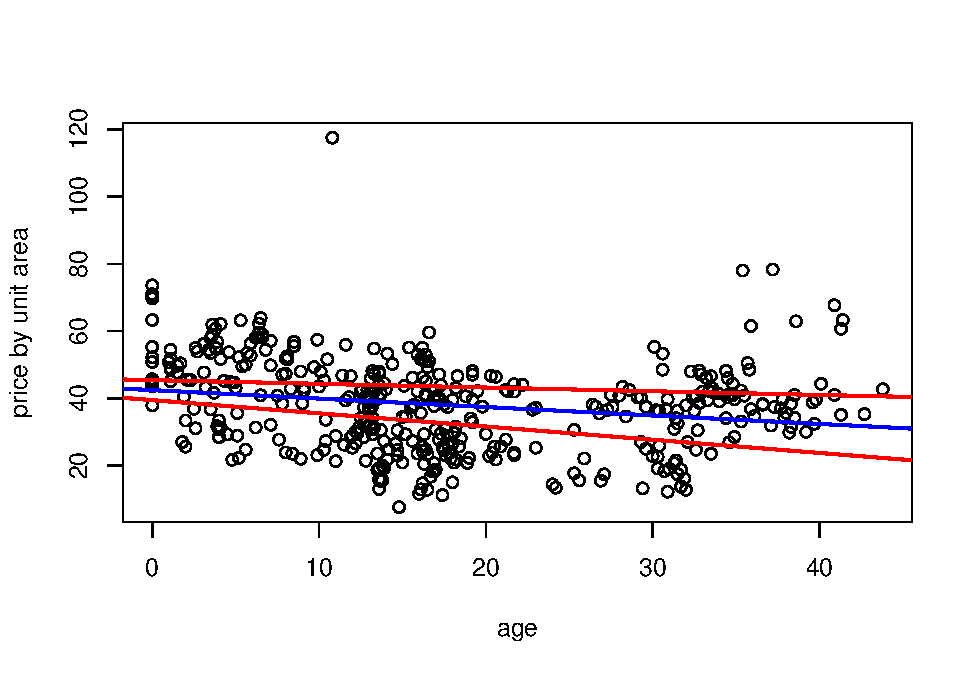
\includegraphics{15-Regression_files/figure-latex/unnamed-chunk-10-1.pdf}

Pointwise confidence bands using CIs for conditional mean responses:

\begin{Shaded}
\begin{Highlighting}[]
\NormalTok{my.summ }\OtherTok{\textless{}{-}} \FunctionTok{summary}\NormalTok{(my.lm)}
\NormalTok{MSE }\OtherTok{\textless{}{-}}\NormalTok{ my.summ}\SpecialCharTok{$}\NormalTok{sigma}\SpecialCharTok{\^{}}\DecValTok{2}
\NormalTok{n}\OtherTok{\textless{}{-}} \FunctionTok{length}\NormalTok{(houses}\SpecialCharTok{$}\NormalTok{Y.house.price.of.unit.area)}
\NormalTok{CI.fun }\OtherTok{\textless{}{-}} \ControlFlowTok{function}\NormalTok{(x)\{}
\NormalTok{  se.term }\OtherTok{\textless{}{-}} \DecValTok{1}\SpecialCharTok{/}\NormalTok{n }\SpecialCharTok{+}\NormalTok{ ((x}\SpecialCharTok{{-}}\FunctionTok{mean}\NormalTok{(houses}\SpecialCharTok{$}\NormalTok{X2.house.age))}\SpecialCharTok{\^{}}\DecValTok{2}\NormalTok{) }\SpecialCharTok{/} \FunctionTok{sum}\NormalTok{((houses}\SpecialCharTok{$}\NormalTok{X2.house.age }\SpecialCharTok{{-}} \FunctionTok{mean}\NormalTok{(houses}\SpecialCharTok{$}\NormalTok{X2.house.age))}\SpecialCharTok{\^{}}\DecValTok{2}\NormalTok{)}
\NormalTok{  ci }\OtherTok{\textless{}{-}} \FunctionTok{c}\NormalTok{(my.summ}\SpecialCharTok{$}\NormalTok{coefficients[}\DecValTok{1}\NormalTok{] }\SpecialCharTok{+}\NormalTok{ my.summ}\SpecialCharTok{$}\NormalTok{coefficients[}\DecValTok{2}\NormalTok{]}\SpecialCharTok{*}\NormalTok{x }\SpecialCharTok{+} \FunctionTok{qt}\NormalTok{(}\FloatTok{0.025}\NormalTok{, my.summ}\SpecialCharTok{$}\NormalTok{df[}\DecValTok{2}\NormalTok{])}\SpecialCharTok{*}\FunctionTok{sqrt}\NormalTok{(MSE}\SpecialCharTok{*}\NormalTok{se.term), my.summ}\SpecialCharTok{$}\NormalTok{coefficients[}\DecValTok{1}\NormalTok{] }\SpecialCharTok{+}\NormalTok{ my.summ}\SpecialCharTok{$}\NormalTok{coefficients[}\DecValTok{2}\NormalTok{]}\SpecialCharTok{*}\NormalTok{x }\SpecialCharTok{+} \FunctionTok{qt}\NormalTok{(}\FloatTok{0.975}\NormalTok{, my.summ}\SpecialCharTok{$}\NormalTok{df[}\DecValTok{2}\NormalTok{])}\SpecialCharTok{*}\FunctionTok{sqrt}\NormalTok{(MSE}\SpecialCharTok{*}\NormalTok{se.term))}
  \FunctionTok{return}\NormalTok{(ci)}
\NormalTok{\}}
\end{Highlighting}
\end{Shaded}

Pointwise intervals in green:

\begin{Shaded}
\begin{Highlighting}[]
\NormalTok{houses }\OtherTok{\textless{}{-}} \FunctionTok{read.csv}\NormalTok{(}\StringTok{"Real estate.csv"}\NormalTok{, }\AttributeTok{header =} \ConstantTok{TRUE}\NormalTok{)}
\FunctionTok{plot}\NormalTok{(houses}\SpecialCharTok{$}\NormalTok{X2.house.age, houses}\SpecialCharTok{$}\NormalTok{Y.house.price.of.unit.area, }\AttributeTok{xlab =} \StringTok{\textquotesingle{}age\textquotesingle{}}\NormalTok{, }\AttributeTok{ylab =} \StringTok{\textquotesingle{}price by unit area\textquotesingle{}}\NormalTok{)}
\FunctionTok{abline}\NormalTok{(}\AttributeTok{a =} \FloatTok{42.43470}\NormalTok{, }\AttributeTok{b =} \SpecialCharTok{{-}}\NormalTok{.}\DecValTok{25149}\NormalTok{, }\AttributeTok{col =} \StringTok{\textquotesingle{}blue\textquotesingle{}}\NormalTok{, }\AttributeTok{lwd =} \DecValTok{2}\NormalTok{)}

\NormalTok{x.seq }\OtherTok{\textless{}{-}} \FunctionTok{seq}\NormalTok{(}\AttributeTok{from =} \DecValTok{0}\NormalTok{, }\AttributeTok{to =} \DecValTok{50}\NormalTok{, }\AttributeTok{length.out =} \DecValTok{400}\NormalTok{)}
\NormalTok{app.fun }\OtherTok{\textless{}{-}} \FunctionTok{apply}\NormalTok{(}\FunctionTok{matrix}\NormalTok{(x.seq, }\DecValTok{400}\NormalTok{,}\DecValTok{1}\NormalTok{),}\DecValTok{1}\NormalTok{,CI.fun)}
\FunctionTok{lines}\NormalTok{(x.seq, app.fun[}\DecValTok{1}\NormalTok{,], }\AttributeTok{col =} \StringTok{\textquotesingle{}green\textquotesingle{}}\NormalTok{, }\AttributeTok{lwd =} \DecValTok{2}\NormalTok{)}
\FunctionTok{lines}\NormalTok{(x.seq, app.fun[}\DecValTok{2}\NormalTok{,], }\AttributeTok{col =} \StringTok{\textquotesingle{}green\textquotesingle{}}\NormalTok{, }\AttributeTok{lwd =} \DecValTok{2}\NormalTok{)}
\FunctionTok{abline}\NormalTok{(}\AttributeTok{a =}\NormalTok{ beta0.intv[}\DecValTok{1}\NormalTok{], }\AttributeTok{b =}\NormalTok{ beta1.intv[}\DecValTok{1}\NormalTok{], }\AttributeTok{col =} \StringTok{\textquotesingle{}red\textquotesingle{}}\NormalTok{, }\AttributeTok{lwd =} \DecValTok{2}\NormalTok{)}
\FunctionTok{abline}\NormalTok{(}\AttributeTok{a =}\NormalTok{ beta0.intv[}\DecValTok{2}\NormalTok{], }\AttributeTok{b =}\NormalTok{ beta1.intv[}\DecValTok{2}\NormalTok{], }\AttributeTok{col =} \StringTok{\textquotesingle{}red\textquotesingle{}}\NormalTok{, }\AttributeTok{lwd =} \DecValTok{2}\NormalTok{)}
\end{Highlighting}
\end{Shaded}

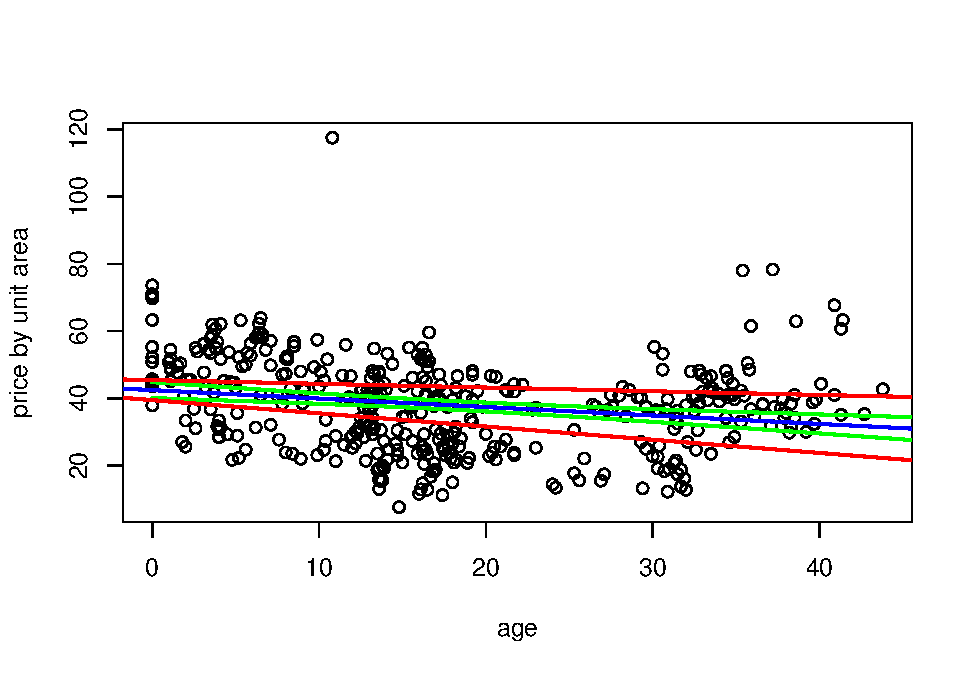
\includegraphics{15-Regression_files/figure-latex/unnamed-chunk-12-1.pdf}

\hypertarget{multiple-linear-regression}{%
\chapter{Multiple Linear Regression}\label{multiple-linear-regression}}

In this chapter we extend the simple linear regression model to accomodate multiple covariates \(X_1, \ldots, X_p\) to better predict the response \(Y\).

\hypertarget{the-multiple-linear-regression-model}{%
\section{The Multiple Linear Regression Model}\label{the-multiple-linear-regression-model}}

Multiple linear regression is a model for predicting the behavior of a response variable \(Y\) using several predictors (also called covariates or explanatory variables) \(X_1, \ldots, X_p\) assumed to have some influence on the response. In particular, the model is linear:
\[Y_i = \beta_0 + \beta_1 X_{1,i} + \beta_2 X_{2,i} + \cdots + \beta_p X_{p,i} + \epsilon_i\]
for \(i=1, \ldots, n\) responses. We assume the random residuals \(\epsilon_i\) are a normal random sample with mean zero and constant variance \(\sigma^2\).

It is convenient to write the multiple linear regression model in matrix-vector form:
\[Y = X\beta+\epsilon\]
where \(Y\) is the \(n\times 1\) vector of response variables, \(X\) is the \(n \times (p+1)\) matrix consisting of an \(n\times 1\) column vector of 1's and the \(p\) columns of predictor variables, where \(\beta\) is a \((p+1) \times 1\) vector of unknown coefficients, and where \(\epsilon\) is the \(n\times 1\) vector of random residuals.

\hypertarget{point-estimation}{%
\section{Point estimation}\label{point-estimation}}

Just as in simple linear regression, we estimate \(\beta\) using the method of least squares. Define the observed residuals

\[e(\hat\beta) = Y_i - X_i^\top\hat\beta\]

where \(\hat\beta\) is some particular value of the vector \(\beta\) and \(X_i\) is the \(i^{th}\) row of the ``design matrix'' \(X\) defined above. Then, the sum of squared observed residuals (often called sum of squares errors) is
\[SSE = \sum_{i=1}^n \left(Y_i - X_i^\top\hat\beta\right)^2.\]
In matrix-vector notation, the SSE is an inner product (dot product):
\[SSE = (Y-X\hat\beta)^\top (Y-X\hat\beta).\]

The method of least squares says that we should choose the estimator \(\hat\beta\) to be the value minimizing the SSE. And, just as in simple linear regression, we can compute this minimizer using calculus. In multiple linear regression, the calculus is a bit more complicated, because we are dealing with vector rather than scalar quantities. To compute the least squares estimator, begin by expanding SSE:
\begin{align*}
SSE &= (Y-X\hat\beta)^\top (Y-X\hat\beta)\\
& = Y^\top Y - Y^\top X\beta - \beta^\top X^\top Y + \hat\beta^\top X^\top X\beta
\end{align*}
Next, differentiate term by term, using the following facts from calculus: for \(n \times 1\) vectors \(a\) and \(x\)
\[\frac{\partial}{\partial x} a^\top x = a^\top;\]
and, for an \(n\times n\) matrix \(A\):
\[\frac{\partial}{\partial x}  x^\top A x = (A + A^\top) x.\]
Applying these rules, we obtain
\begin{align*}
\frac{\partial}{\partial \beta} SSE &= -Y^\top X - (Y^\top X)^\top + (X^\top X + X^\top X) \beta\\
& = 2X^\top X \beta - 2X^\top Y
\end{align*}
If \(X^\top X\) is invertible, we may set this equation equal to the \((p+1)\times 1\) zero vector and solve, obtaining
\[\hat\beta = (X^\top X)^{-1}X^\top Y.\]
Just as in simple linear regression, our least squares estimator is unbiased:
\[E(\hat\beta) = E((X^\top X)^{-1}X^\top Y) = (X^\top X)^{-1}X^\top X\beta = \beta.\]
To estimate \(\sigma^2\), we use (an adjustment to) the method of moments,
\[\hat\sigma^2 = \frac{1}{n-(p+1)}SSE = \frac{1}{n-(p+1)}(Y - X\hat\beta)^\top(Y - X\hat\beta).\]
This estimator is also unbiased, i.e., \(E(\hat\sigma^2) = \sigma^2\).

\hypertarget{sampling-distributions-1}{%
\section{Sampling Distributions}\label{sampling-distributions-1}}

The estimated regression coefficients have a multivariate normal distribution due to the fact they are equal to linear combinations of the normally-distributed responses:
\[\hat\beta \sim N_{p+1}\left(\beta, \sigma^2 (X^\top X)^{-1}\right).\]
This means the least squares estimator is normally distributed, unbiased, and has covariance matrix \(\sigma^2 (X^\top X)^{-1}\). For example, \(V(\hat\beta_j) = \sigma^2 (X^\top X)^{-1}_{j,j}\), which is the variance parameter \(\sigma^2\) multiplies by the \(j^{th}\) diagonal entry of the matrix \((X^\top X)^{-1}\).

The variance estimator \(\hat\sigma^2\) (properly scaled) has a Chi-Squared distribution:
\[\frac{[n-(p+1)]\hat\sigma^2}{\sigma^2}\sim \chi^2( n - p - 1).\]

Furthermore, the least squares estimator is independent of the variance estimator, which implies the Studentized estimated coefficients are \(t-\)distributed:
\[\frac{\hat\beta_j - \beta_j}{\sqrt{\hat\sigma^2 (X^\top X)^{-1}_{j,j}}}\sim t_{n-p-1}.\]

\hypertarget{inference-on-regression-coefficients}{%
\section{Inference on regression coefficients}\label{inference-on-regression-coefficients}}

The Student's t sampling distribution noted above enables us to derive exact confidence intervals and hypothesis tests for individual regression coefficients. A \(100(1-\alpha)\%\) CI for \(\beta_j\) is given by
\[(\hat\beta_j \pm t_{1-\alpha/2, n-p-1}\sqrt{\hat\sigma^2 (X^\top X)^{-1}_{j,j}}).\]
To test \(H_0:\beta_j = 0\) versus \(H_a:\beta_j\ne 0\) we reject the null hypothesis at level \(\alpha\) if \(|t| > t_{1-\alpha.2, n-p-1}\) where
\[t = \frac{\hat\beta_j - 0}{\sqrt{\hat\sigma^2 (X^\top X)^{-1}_{j,j}}}.\]
The interpretation of the above null hypothesis is that including covariate \(X_j\) in the model does not significantly improve accuracy of predicting \(Y\).

We can also test for significance/insignificance of several covariates at a time using \emph{partial F tests}. Let \(X^R\) denote a subset of the columns of the design matrix \(X\) where we have removed columns corresponding to a subset of \(r\) of the coefficients in \(\beta\). Fit the model \(Y = X^R\beta^R + \epsilon\) and compute the sum of squared residuals for this \textbf{reduced} model, call it, \(\text{SSE}^R\). Let \(\text{SSE}^F\) denote the sum of squared residuals for the \textbf{full} model with all \(p\) covariates. Define
\[F = \frac{(SSE^R - SSE^F)/r }{SSE^F / (n-p-1)}.\]
Then, under \(H_0:\text{all of these }r\text{ covariates have coefficients equal to zero}\) we have \(F\sim F_{r, n-p-1}\), that is, the test statistic \(F\) has an \(F\) distribution with numerator and denominator degrees of freedom \(r\) and \(n-p-1\). We reject the null hypothesis at level \(\alpha\) if \(F > F_{1-\alpha, r, n-p-1}\).

\hypertarget{example-housing-price-data}{%
\subsection{Example: Housing price data}\label{example-housing-price-data}}

\begin{Shaded}
\begin{Highlighting}[]
\NormalTok{houses }\OtherTok{\textless{}{-}} \FunctionTok{read.csv}\NormalTok{(}\StringTok{"Real estate.csv"}\NormalTok{, }\AttributeTok{header =} \ConstantTok{TRUE}\NormalTok{)}
\FunctionTok{colnames}\NormalTok{(houses) }\OtherTok{\textless{}{-}} \FunctionTok{c}\NormalTok{(}\StringTok{\textquotesingle{}date\textquotesingle{}}\NormalTok{, }\StringTok{\textquotesingle{}age\textquotesingle{}}\NormalTok{, }\StringTok{\textquotesingle{}distance\_to\_transit\textquotesingle{}}\NormalTok{, }\StringTok{\textquotesingle{}num\_stores\textquotesingle{}}\NormalTok{, }\StringTok{\textquotesingle{}lat\textquotesingle{}}\NormalTok{, }\StringTok{\textquotesingle{}long\textquotesingle{}}\NormalTok{, }\StringTok{\textquotesingle{}price\_per\_unit\_area\textquotesingle{}}\NormalTok{)}
\end{Highlighting}
\end{Shaded}

Let's fit a multiple linear regression model to predict price per unit area using a house's age, its distance to the nearest transit station, and the number of nearby convenience stores. Intuitively, age affects a home's value, while the other two variables have to do with the value of the location and neighborhood.

\begin{Shaded}
\begin{Highlighting}[]
\NormalTok{my.lm }\OtherTok{\textless{}{-}} \FunctionTok{lm}\NormalTok{(price\_per\_unit\_area}\SpecialCharTok{\textasciitilde{}}\NormalTok{age}\SpecialCharTok{+}\NormalTok{distance\_to\_transit}\SpecialCharTok{+}\NormalTok{num\_stores, }\AttributeTok{data =}\NormalTok{ houses)}
\FunctionTok{summary}\NormalTok{(my.lm)}
\end{Highlighting}
\end{Shaded}

\begin{verbatim}
## 
## Call:
## lm(formula = price_per_unit_area ~ age + distance_to_transit + 
##     num_stores, data = houses)
## 
## Residuals:
##       Min        1Q    Median        3Q       Max 
## -0.013025 -0.003845 -0.000584  0.002303  0.052341 
## 
## Coefficients:
##                       Estimate Std. Error t value Pr(>|t|)    
## (Intercept)          1.206e+02  3.203e+00   37.65   <2e-16 ***
## age                  4.619e-04  1.591e-03    0.29    0.772    
## distance_to_transit -3.774e-05  3.932e-05   -0.96    0.338    
## num_stores          -9.802e-06  3.555e-07  -27.57   <2e-16 ***
## ---
## Signif. codes:  0 '***' 0.001 '**' 0.01 '*' 0.05 '.' 0.1 ' ' 1
## 
## Residual standard error: 0.0091 on 410 degrees of freedom
## Multiple R-squared:  0.651,  Adjusted R-squared:  0.6484 
## F-statistic: 254.9 on 3 and 410 DF,  p-value: < 2.2e-16
\end{verbatim}

The fitted regression line is
\[\text{price per unit area} = 120.6 + 0.0004619 \times \text{age} - 0.00003774 \times \text{distance to transit} - 0.000009802 \times \text{number of stores}.\]
However, t-tests suggest that neither the inclusion of age nor distance to transit in the model are improving the price predictions (p-values are 0.772 and 0.338).

\begin{Shaded}
\begin{Highlighting}[]
\NormalTok{X }\OtherTok{\textless{}{-}} \FunctionTok{model.matrix}\NormalTok{(price\_per\_unit\_area}\SpecialCharTok{\textasciitilde{}}\NormalTok{age}\SpecialCharTok{+}\NormalTok{distance\_to\_transit}\SpecialCharTok{+}\NormalTok{num\_stores, }\AttributeTok{data =}\NormalTok{ houses)}
\NormalTok{hat.sigma2 }\OtherTok{\textless{}{-}} \FunctionTok{summary}\NormalTok{(my.lm)}\SpecialCharTok{$}\NormalTok{sigma}\SpecialCharTok{\^{}}\DecValTok{2}
\NormalTok{cov.beta }\OtherTok{\textless{}{-}}\NormalTok{ hat.sigma2}\SpecialCharTok{*}\FunctionTok{solve}\NormalTok{(}\FunctionTok{t}\NormalTok{(X)}\SpecialCharTok{\%*\%}\NormalTok{X)}
\NormalTok{cov.beta[}\DecValTok{2}\NormalTok{,}\DecValTok{3}\NormalTok{]}\SpecialCharTok{/}\FunctionTok{sqrt}\NormalTok{(cov.beta[}\DecValTok{2}\NormalTok{,}\DecValTok{2}\NormalTok{]}\SpecialCharTok{*}\NormalTok{cov.beta[}\DecValTok{3}\NormalTok{,}\DecValTok{3}\NormalTok{])}
\end{Highlighting}
\end{Shaded}

\begin{verbatim}
## [1] -0.01602387
\end{verbatim}

\begin{Shaded}
\begin{Highlighting}[]
\NormalTok{cov.beta[}\DecValTok{2}\NormalTok{,}\DecValTok{4}\NormalTok{]}\SpecialCharTok{/}\FunctionTok{sqrt}\NormalTok{(cov.beta[}\DecValTok{2}\NormalTok{,}\DecValTok{2}\NormalTok{]}\SpecialCharTok{*}\NormalTok{cov.beta[}\DecValTok{4}\NormalTok{,}\DecValTok{4}\NormalTok{])}
\end{Highlighting}
\end{Shaded}

\begin{verbatim}
## [1] -0.06045947
\end{verbatim}

\begin{Shaded}
\begin{Highlighting}[]
\NormalTok{cov.beta[}\DecValTok{3}\NormalTok{,}\DecValTok{4}\NormalTok{]}\SpecialCharTok{/}\FunctionTok{sqrt}\NormalTok{(cov.beta[}\DecValTok{3}\NormalTok{,}\DecValTok{3}\NormalTok{]}\SpecialCharTok{*}\NormalTok{cov.beta[}\DecValTok{4}\NormalTok{,}\DecValTok{4}\NormalTok{])}
\end{Highlighting}
\end{Shaded}

\begin{verbatim}
## [1] -0.0246031
\end{verbatim}

Above we computed the estimated correlation between the coefficients of age, distance to transit, and number of stores. These estimated correlations are all close to zero, meaning the estimated coefficients are not correlated. When estimated coefficients are strongly correlated, it is challenging to interpret the multiple linear regression model. For example, the estimate of \(\hat\beta_1 = 0.0004619\) means that for a one unit increase in age, the home price by unit area increases by 0.0004619 units \textbf{provided all other covariates are held constant}. If the covariates are not correlated, this explanation makes sense. However, if two covariates are strongly, say, positively correlated, then when one goes up it must be that the other goes up as well, so it is not reasonable to assume one can be changed while the other is held constant. Correlation of the covariates is called \emph{multicollinearity} and it is important to check for multicollinearity before attempting to interpret coefficients as above.

Note that the summary of the lm function call includes an F test result in the last line. It says ``F-statistic: 254.9 on 3 and 410 DF, p-value: \textless{} 2.2e-16''. This is called the \emph{model F test} and it is a partial F test of the hypothesis that only the intercept coefficient is non zero, i.e.~\(\beta_0 \ne 0\) but \(\beta_j = 0\) for all \(j > 0\). We can match this F test result by fitting the ``intercept-only'' model and comparing SSEs:

\begin{Shaded}
\begin{Highlighting}[]
\NormalTok{my.lm.int }\OtherTok{\textless{}{-}} \FunctionTok{lm}\NormalTok{(price\_per\_unit\_area}\SpecialCharTok{\textasciitilde{}}\DecValTok{1}\NormalTok{, }\AttributeTok{data =}\NormalTok{ houses)}
\NormalTok{SSE.R }\OtherTok{\textless{}{-}} \FunctionTok{sum}\NormalTok{(my.lm.int}\SpecialCharTok{$}\NormalTok{residuals}\SpecialCharTok{\^{}}\DecValTok{2}\NormalTok{)}
\NormalTok{SSE.F }\OtherTok{\textless{}{-}} \FunctionTok{sum}\NormalTok{(my.lm}\SpecialCharTok{$}\NormalTok{residuals}\SpecialCharTok{\^{}}\DecValTok{2}\NormalTok{)}
\NormalTok{n }\OtherTok{\textless{}{-}} \FunctionTok{length}\NormalTok{(houses}\SpecialCharTok{$}\NormalTok{price\_per\_unit\_area)}

\NormalTok{F }\OtherTok{\textless{}{-}}\NormalTok{ ((SSE.R }\SpecialCharTok{{-}}\NormalTok{ SSE.F)}\SpecialCharTok{/}\DecValTok{3}\NormalTok{)}\SpecialCharTok{/}\NormalTok{(SSE.F }\SpecialCharTok{/}\NormalTok{ (n}\DecValTok{{-}4}\NormalTok{))}
\NormalTok{F}
\end{Highlighting}
\end{Shaded}

\begin{verbatim}
## [1] 254.923
\end{verbatim}

\begin{Shaded}
\begin{Highlighting}[]
\DecValTok{1}\SpecialCharTok{{-}}\FunctionTok{pf}\NormalTok{(F,}\DecValTok{3}\NormalTok{,n}\DecValTok{{-}4}\NormalTok{)}
\end{Highlighting}
\end{Shaded}

\begin{verbatim}
## [1] 0
\end{verbatim}

\hypertarget{likelihood-based-inferences}{%
\chapter{Likelihood-Based Inferences}\label{likelihood-based-inferences}}

Previously, we discussed approximate sampling distribution theory for maximum likelihood estimators. Recall that if \(\hat\theta\) is the MLE of \(\theta\), the parameter of a distribution family \(P_\theta\), then (under some technical conditions)
\[\hat\theta \stackrel{\cdot}{\sim} N(\theta, I(\theta)^{-1})\]
for large \(n\) where \(I(\theta)\) is the Fisher information
\[I(\theta) = -E\left[\frac{\partial^2}{\partial \theta} \ell(\theta;X_1, \ldots, X_n)\right]\]
for a random sample \(X_1,\ldots, X_n\) from \(P_\theta\).

In this chapter we discuss how to use this (and other) approximate (large sample) sampling distributions to make inferences about population parameters.

\hypertarget{wald-tests-and-cis}{%
\section{Wald tests and CIs}\label{wald-tests-and-cis}}

A \(100(1-\alpha)\%\) Wald approximate CI for a scalar parameter \(\theta\) has the form
\[\left(\hat\theta \pm z_{1-\alpha/2}\sqrt{I(\hat\theta)^{-1}}\right)\]

This CI is straightforward to obtain by the same argument we have used before. Start with the identity
\[1-\alpha \approx P\left(z_{\alpha/2} < \frac{\hat\theta - \theta}{\sqrt{I(\theta)^{-1}}} < z_{1-\alpha/2}\right)\]
which follows from the approximate pivot discussed above, and in Chapter 2. Then, simply multiply by the standard error \(\sqrt{I(\theta)^{-1}}\), subtract \(\hat\theta\) from both sides, and multiply by \(-1\) to get
\[1-\alpha \approx P\left(\hat\theta - z_{1-\alpha/2}\sqrt{I(\theta)^{-1}} < \theta < \hat\theta + z_{1-\alpha/2}\sqrt{I(\theta)^{-1}}\right)\]
Finally, since \(\theta\) is unknown, replace \(\theta\) by \(\hat\theta\) in the standard error to yield the so-called Wald type CI
\[\left(\hat\theta \pm z_{1-\alpha/2}\sqrt{I(\hat\theta)^{-1}}\right).\]

If \(\theta = (\theta_1, \ldots, \theta_p)\) is a vector, then, the marginal Wald approximate CI for \(\theta_j\) is given by
\[\left(\hat\theta_j \pm z_{1-\alpha/2}\sqrt{I(\hat\theta)_{j,j}^{-1}}\right).\]
where \(I(\theta)\) is the Fisher information \emph{matrix} and \(I(\theta)_{j,j}\) is the \(j^{th}\) diagonal entry of the Fisher information matrix.

Besides CIs, the approximate pivot may be used for hypothesis tests as well. To test \(H_0:\theta = \theta_0\) versus \(H_a: \theta\ne \theta_0\) for a scalar parameter \(\theta\), reject the null hypothesis if \(|z| > z_{1-\alpha/2}\) where
\[z=\frac{\hat\theta - \theta_0}{\sqrt{I(\theta_0)^{-1}}}.\]
(Alternatively, one may use \(\hat\theta\) in the standard error rather than \(\theta_0\). Under the null hypothesis, there is little difference.)

For a vector parameter \(\theta\) let
\[W = (\hat\theta - \theta_0)^\top I(\theta_0)^{-1}(\hat\theta - \theta_0).\]
Under \(H_0:\theta = \theta_0\), \(W\stackrel{\cdot}{\sim}\chi^2(p)\). And, if we use the estimated covariance:
\[V = (\hat\theta - \theta_0)^\top I(\hat\theta)^{-1}(\hat\theta - \theta_0),\]
then, \(V\stackrel{\cdot}{\sim} F(p, n-p)\). So, we get either a Chi-Squared or F-based test for a vector parameter.

\hypertarget{example-auto-insurance-claims}{%
\subsection{Example: Auto insurance claims}\label{example-auto-insurance-claims}}

We have the following data on 100 auto insurance claims:

\includegraphics{17-LikelihoodInference_files/figure-latex/unnamed-chunk-2-1.pdf}

Given the auto claims are positively skewed, we will assume a Gamma distribution reasonably models the population and fit a Gamma to the data by maximum likelihood.

The Gamma density has form
\[f(x;\alpha, \beta) = \frac{\beta^\alpha}{\Gamma(\alpha)}x^{\alpha-1}e^{-x\beta}, \quad x,\alpha, \beta>0\]
where \((\alpha, \beta)\) are shape and rate parameters. The likelihood for a random sample of size \(n\) is
\[L(\alpha, \beta; X_1, \ldots, X_n) = \left(\frac{\beta^\alpha}{\Gamma(\alpha)}\right)^n \prod_{i=1}^n (x_i)^{\alpha - 1} e^{-\beta\sum_{i=1}^n x_i}.\]
Taking the log, we have the loglikelihood function (suppressing dependence on data)
\[\ell(\alpha, \beta) = n\alpha\log \beta - n\log \Gamma(\alpha) + (\alpha - 1)\sum_{i=1}^n \log(x_i) - \beta\sum_{i=1}^n x_i.\]
Next, we need the gradient (the first derivatives) w.r.t. the parameters \((\alpha,\beta)\):
\[\frac{\partial \ell}{\partial \alpha} = n\log\beta - \text{DiGamma}(\alpha) + \sum_{i=1}^n \log(x_i)\]
where the function DiGamma\((\alpha)\) is the logarithmic derivative of the Gamma function. Next, we have
\[\frac{\partial \ell}{\partial \beta} = \frac{n\alpha}{\beta} - \sum_{i=1}^n x_i.\]

We also need the second derivatives in order to compute the Fisher information:
\[\frac{\partial^2 \ell}{\partial \alpha^2} = -\text{TriGamma}(\alpha)\]
where the TriGamma function is (you guessed it!) the second logarithmic derivative fo the Gamma function \(\Gamma(\alpha)\).\\
\[\frac{\partial^2 \ell}{\partial \alpha\partial\beta} = n/\beta.\]
\[\frac{\partial^2 \ell}{\partial \beta^2} = -\frac{n\alpha}{\beta^2}.\]

You may have guessed we will not be able to compute the MLEs by hand by solving \(\frac{\partial \ell}{\partial \alpha}=0\) and \(\frac{\partial \ell}{\partial \beta} = 0\). Instead, we need an iterative solver (an algorithm). In R we can use \emph{optim} to solve for the MLEs. Or, we can code our own version of Newton's method\ldots{}

\begin{Shaded}
\begin{Highlighting}[]
\NormalTok{n }\OtherTok{\textless{}{-}} \FunctionTok{length}\NormalTok{(data)}
\NormalTok{loglik }\OtherTok{\textless{}{-}} \ControlFlowTok{function}\NormalTok{(param)\{}
  \FunctionTok{sum}\NormalTok{(}\FunctionTok{dgamma}\NormalTok{(data, }\AttributeTok{shape =}\NormalTok{ param[}\DecValTok{1}\NormalTok{], }\AttributeTok{rate =}\NormalTok{ param[}\DecValTok{2}\NormalTok{], }\AttributeTok{log =} \ConstantTok{TRUE}\NormalTok{))}
\NormalTok{\}}
\NormalTok{grad }\OtherTok{\textless{}{-}} \ControlFlowTok{function}\NormalTok{(param)\{}
\NormalTok{  g1 }\OtherTok{\textless{}{-}}\NormalTok{ n}\SpecialCharTok{*}\FunctionTok{log}\NormalTok{(param[}\DecValTok{2}\NormalTok{]) }\SpecialCharTok{{-}} \FunctionTok{digamma}\NormalTok{(param[}\DecValTok{1}\NormalTok{]) }\SpecialCharTok{+} \FunctionTok{sum}\NormalTok{(}\FunctionTok{log}\NormalTok{(data))}
\NormalTok{  g2 }\OtherTok{\textless{}{-}}\NormalTok{ n}\SpecialCharTok{*}\NormalTok{param[}\DecValTok{1}\NormalTok{]}\SpecialCharTok{/}\NormalTok{param[}\DecValTok{2}\NormalTok{] }\SpecialCharTok{{-}} \FunctionTok{sum}\NormalTok{(data)}
  \FunctionTok{return}\NormalTok{(}\FunctionTok{c}\NormalTok{(g1,g2))}
\NormalTok{\}}
\NormalTok{H }\OtherTok{\textless{}{-}} \ControlFlowTok{function}\NormalTok{(param)\{}
\NormalTok{  h1 }\OtherTok{\textless{}{-}} \SpecialCharTok{{-}}\FunctionTok{trigamma}\NormalTok{(param[}\DecValTok{1}\NormalTok{])}
\NormalTok{  h2 }\OtherTok{\textless{}{-}}\NormalTok{ n}\SpecialCharTok{/}\NormalTok{param[}\DecValTok{2}\NormalTok{]}
\NormalTok{  h3 }\OtherTok{\textless{}{-}} \SpecialCharTok{{-}}\NormalTok{n}\SpecialCharTok{*}\NormalTok{param[}\DecValTok{1}\NormalTok{]}\SpecialCharTok{/}\NormalTok{(param[}\DecValTok{2}\NormalTok{]}\SpecialCharTok{\^{}}\DecValTok{2}\NormalTok{)}
  \FunctionTok{return}\NormalTok{(}\FunctionTok{matrix}\NormalTok{(}\FunctionTok{c}\NormalTok{(h1,h2,h2,h3),}\DecValTok{2}\NormalTok{,}\DecValTok{2}\NormalTok{))}
\NormalTok{\}}

\NormalTok{m }\OtherTok{\textless{}{-}} \FunctionTok{mean}\NormalTok{(data)}
\NormalTok{v }\OtherTok{\textless{}{-}} \FunctionTok{var}\NormalTok{(data)}

\NormalTok{beta0 }\OtherTok{\textless{}{-}}\NormalTok{ m}\SpecialCharTok{/}\NormalTok{v}
\NormalTok{alpha0 }\OtherTok{\textless{}{-}}\NormalTok{ m}\SpecialCharTok{*}\NormalTok{beta0}

\NormalTok{delta }\OtherTok{\textless{}{-}} \FloatTok{0.00001}
\NormalTok{diff.step }\OtherTok{\textless{}{-}} \DecValTok{1}
\NormalTok{par.old }\OtherTok{\textless{}{-}} \FunctionTok{c}\NormalTok{(alpha0, beta0)}
\NormalTok{steps }\OtherTok{\textless{}{-}} \DecValTok{0}
\ControlFlowTok{while}\NormalTok{((diff.step }\SpecialCharTok{\textgreater{}}\NormalTok{ delta) }\SpecialCharTok{\&}\NormalTok{ (steps }\SpecialCharTok{\textless{}} \DecValTok{100}\NormalTok{))\{}
\NormalTok{  par.new }\OtherTok{\textless{}{-}}\NormalTok{ par.old }\SpecialCharTok{{-}} \FunctionTok{solve}\NormalTok{(}\FunctionTok{H}\NormalTok{(par.old))}\SpecialCharTok{\%*\%}\FunctionTok{matrix}\NormalTok{(}\FunctionTok{grad}\NormalTok{(par.old),}\DecValTok{2}\NormalTok{,}\DecValTok{1}\NormalTok{) }
\NormalTok{  diff.step }\OtherTok{\textless{}{-}} \FunctionTok{max}\NormalTok{(}\FunctionTok{abs}\NormalTok{(par.new }\SpecialCharTok{{-}}\NormalTok{ par.old))}
\NormalTok{  steps }\OtherTok{\textless{}{-}}\NormalTok{ steps }\SpecialCharTok{+} \DecValTok{1}
\NormalTok{  par.old }\OtherTok{\textless{}{-}}\NormalTok{ par.new}
\NormalTok{\}}
\NormalTok{par.old}
\end{Highlighting}
\end{Shaded}

\begin{verbatim}
##             [,1]
## [1,] 1.314900300
## [2,] 0.001302721
\end{verbatim}

\begin{Shaded}
\begin{Highlighting}[]
\FunctionTok{loglik}\NormalTok{(par.old)}
\end{Highlighting}
\end{Shaded}

\begin{verbatim}
## [1] -784.811
\end{verbatim}

\begin{Shaded}
\begin{Highlighting}[]
\FunctionTok{H}\NormalTok{(par.old)}
\end{Highlighting}
\end{Shaded}

\begin{verbatim}
##              [,1]        [,2]
## [1,]    -1.116659     76762.4
## [2,] 76762.401301 -77480056.4
\end{verbatim}

\begin{Shaded}
\begin{Highlighting}[]
\FunctionTok{solve}\NormalTok{(}\FunctionTok{H}\NormalTok{(par.old))}
\end{Highlighting}
\end{Shaded}

\begin{verbatim}
##              [,1]         [,2]
## [1,] 1.334495e-02 1.322134e-05
## [2,] 1.322134e-05 1.923302e-10
\end{verbatim}

\begin{Shaded}
\begin{Highlighting}[]
\NormalTok{mle.optim }\OtherTok{\textless{}{-}} \FunctionTok{optim}\NormalTok{(}\FunctionTok{c}\NormalTok{(alpha0, beta0), loglik, }\AttributeTok{gr =}\NormalTok{ grad, }\AttributeTok{control =} \FunctionTok{list}\NormalTok{(}\AttributeTok{fnscale =} \SpecialCharTok{{-}}\DecValTok{1}\NormalTok{), }\AttributeTok{method =} \StringTok{\textquotesingle{}BFGS\textquotesingle{}}\NormalTok{, }\AttributeTok{hessian =} \ConstantTok{TRUE}\NormalTok{)}
\NormalTok{mle.optim}
\end{Highlighting}
\end{Shaded}

\begin{verbatim}
## $par
## [1] 2.004494690 0.001985928
## 
## $value
## [1] -780.6075
## 
## $counts
## function gradient 
##       23        1 
## 
## $convergence
## [1] 0
## 
## $message
## NULL
## 
## $hessian
##               [,1]         [,2]
## [1,]    -0.6431228     52879.21
## [2,] 52879.2051016 -68089522.01
\end{verbatim}

\begin{Shaded}
\begin{Highlighting}[]
\FunctionTok{solve}\NormalTok{(mle.optim}\SpecialCharTok{$}\NormalTok{hessian)}
\end{Highlighting}
\end{Shaded}

\begin{verbatim}
##              [,1]         [,2]
## [1,] 2.473805e-02 1.921189e-05
## [2,] 1.921189e-05 2.336572e-10
\end{verbatim}

  \bibliography{book.bib,packages.bib}

\end{document}
